%! TEX program = xelatexp
%DIF LATEXDIFF DIFFERENCE FILE
%DIF DEL main_v0.tex   Mon Mar 25 18:35:25 2024
%DIF ADD main.tex      Mon Mar 25 17:21:14 2024
%! TEX encoding = UTF-8 Unicode

\documentclass{elsarticle}
\usepackage{graphicx}
\usepackage{amsmath,amssymb,amsfonts,amsthm,bm}
\usepackage{hyperref}
\usepackage{booktabs,multirow}
\usepackage{lineno}
%DIF 10d10
%DIF < % \usepackage{cite}
%DIF -------
\linenumbers

\bibliographystyle{elsarticle-num}
%DIF < % \biboptions{longnamesfirst,angle,semicolon}
%DIF PREAMBLE EXTENSION ADDED BY LATEXDIFF
%DIF UNDERLINE PREAMBLE %DIF PREAMBLE
\RequirePackage[normalem]{ulem} %DIF PREAMBLE
\RequirePackage{color}\definecolor{RED}{rgb}{1,0,0}\definecolor{BLUE}{rgb}{0,0,1} %DIF PREAMBLE
\providecommand{\DIFaddtex}[1]{{\protect\color{blue}\uwave{#1}}} %DIF PREAMBLE
\providecommand{\DIFdeltex}[1]{{\protect\color{red}\sout{#1}}}                      %DIF PREAMBLE
%DIF SAFE PREAMBLE %DIF PREAMBLE
\providecommand{\DIFaddbegin}{} %DIF PREAMBLE
\providecommand{\DIFaddend}{} %DIF PREAMBLE
\providecommand{\DIFdelbegin}{} %DIF PREAMBLE
\providecommand{\DIFdelend}{} %DIF PREAMBLE
\providecommand{\DIFmodbegin}{} %DIF PREAMBLE
\providecommand{\DIFmodend}{} %DIF PREAMBLE
%DIF FLOATSAFE PREAMBLE %DIF PREAMBLE
\providecommand{\DIFaddFL}[1]{\DIFadd{#1}} %DIF PREAMBLE
\providecommand{\DIFdelFL}[1]{\DIFdel{#1}} %DIF PREAMBLE
\providecommand{\DIFaddbeginFL}{} %DIF PREAMBLE
\providecommand{\DIFaddendFL}{} %DIF PREAMBLE
\providecommand{\DIFdelbeginFL}{} %DIF PREAMBLE
\providecommand{\DIFdelendFL}{} %DIF PREAMBLE
%DIF HYPERREF PREAMBLE %DIF PREAMBLE
\providecommand{\DIFadd}[1]{\texorpdfstring{\DIFaddtex{#1}}{#1}} %DIF PREAMBLE
\providecommand{\DIFdel}[1]{\texorpdfstring{\DIFdeltex{#1}}{}} %DIF PREAMBLE
\newcommand{\DIFscaledelfig}{0.5}
%DIF HIGHLIGHTGRAPHICS PREAMBLE %DIF PREAMBLE
\RequirePackage{settobox} %DIF PREAMBLE
\RequirePackage{letltxmacro} %DIF PREAMBLE
\newsavebox{\DIFdelgraphicsbox} %DIF PREAMBLE
\newlength{\DIFdelgraphicswidth} %DIF PREAMBLE
\newlength{\DIFdelgraphicsheight} %DIF PREAMBLE
% store original definition of \includegraphics %DIF PREAMBLE
\LetLtxMacro{\DIFOincludegraphics}{\includegraphics} %DIF PREAMBLE
\newcommand{\DIFaddincludegraphics}[2][]{{\color{blue}\fbox{\DIFOincludegraphics[#1]{#2}}}} %DIF PREAMBLE
\newcommand{\DIFdelincludegraphics}[2][]{% %DIF PREAMBLE
\sbox{\DIFdelgraphicsbox}{\DIFOincludegraphics[#1]{#2}}% %DIF PREAMBLE
\settoboxwidth{\DIFdelgraphicswidth}{\DIFdelgraphicsbox} %DIF PREAMBLE
\settoboxtotalheight{\DIFdelgraphicsheight}{\DIFdelgraphicsbox} %DIF PREAMBLE
\scalebox{\DIFscaledelfig}{% %DIF PREAMBLE
\parbox[b]{\DIFdelgraphicswidth}{\usebox{\DIFdelgraphicsbox}\\[-\baselineskip] \rule{\DIFdelgraphicswidth}{0em}}\llap{\resizebox{\DIFdelgraphicswidth}{\DIFdelgraphicsheight}{% %DIF PREAMBLE
\setlength{\unitlength}{\DIFdelgraphicswidth}% %DIF PREAMBLE
\begin{picture}(1,1)% %DIF PREAMBLE
\thicklines\linethickness{2pt} %DIF PREAMBLE
{\color[rgb]{1,0,0}\put(0,0){\framebox(1,1){}}}% %DIF PREAMBLE
{\color[rgb]{1,0,0}\put(0,0){\line( 1,1){1}}}% %DIF PREAMBLE
{\color[rgb]{1,0,0}\put(0,1){\line(1,-1){1}}}% %DIF PREAMBLE
\end{picture}% %DIF PREAMBLE
}\hspace*{3pt}}} %DIF PREAMBLE
} %DIF PREAMBLE
\LetLtxMacro{\DIFOaddbegin}{\DIFaddbegin} %DIF PREAMBLE
\LetLtxMacro{\DIFOaddend}{\DIFaddend} %DIF PREAMBLE
\LetLtxMacro{\DIFOdelbegin}{\DIFdelbegin} %DIF PREAMBLE
\LetLtxMacro{\DIFOdelend}{\DIFdelend} %DIF PREAMBLE
\DeclareRobustCommand{\DIFaddbegin}{\DIFOaddbegin \let\includegraphics\DIFaddincludegraphics} %DIF PREAMBLE
\DeclareRobustCommand{\DIFaddend}{\DIFOaddend \let\includegraphics\DIFOincludegraphics} %DIF PREAMBLE
\DeclareRobustCommand{\DIFdelbegin}{\DIFOdelbegin \let\includegraphics\DIFdelincludegraphics} %DIF PREAMBLE
\DeclareRobustCommand{\DIFdelend}{\DIFOaddend \let\includegraphics\DIFOincludegraphics} %DIF PREAMBLE
\LetLtxMacro{\DIFOaddbeginFL}{\DIFaddbeginFL} %DIF PREAMBLE
\LetLtxMacro{\DIFOaddendFL}{\DIFaddendFL} %DIF PREAMBLE
\LetLtxMacro{\DIFOdelbeginFL}{\DIFdelbeginFL} %DIF PREAMBLE
\LetLtxMacro{\DIFOdelendFL}{\DIFdelendFL} %DIF PREAMBLE
\DeclareRobustCommand{\DIFaddbeginFL}{\DIFOaddbeginFL \let\includegraphics\DIFaddincludegraphics} %DIF PREAMBLE
\DeclareRobustCommand{\DIFaddendFL}{\DIFOaddendFL \let\includegraphics\DIFOincludegraphics} %DIF PREAMBLE
\DeclareRobustCommand{\DIFdelbeginFL}{\DIFOdelbeginFL \let\includegraphics\DIFdelincludegraphics} %DIF PREAMBLE
\DeclareRobustCommand{\DIFdelendFL}{\DIFOaddendFL \let\includegraphics\DIFOincludegraphics} %DIF PREAMBLE
%DIF COLORLISTINGS PREAMBLE %DIF PREAMBLE
\RequirePackage{listings} %DIF PREAMBLE
\RequirePackage{color} %DIF PREAMBLE
\lstdefinelanguage{DIFcode}{ %DIF PREAMBLE
%DIF DIFCODE_UNDERLINE %DIF PREAMBLE
  moredelim=[il][\color{red}\sout]{\%DIF\ <\ }, %DIF PREAMBLE
  moredelim=[il][\color{blue}\uwave]{\%DIF\ >\ } %DIF PREAMBLE
} %DIF PREAMBLE
\lstdefinestyle{DIFverbatimstyle}{ %DIF PREAMBLE
	language=DIFcode, %DIF PREAMBLE
	basicstyle=\ttfamily, %DIF PREAMBLE
	columns=fullflexible, %DIF PREAMBLE
	keepspaces=true %DIF PREAMBLE
} %DIF PREAMBLE
\lstnewenvironment{DIFverbatim}{\lstset{style=DIFverbatimstyle}}{} %DIF PREAMBLE
\lstnewenvironment{DIFverbatim*}{\lstset{style=DIFverbatimstyle,showspaces=true}}{} %DIF PREAMBLE
%DIF END PREAMBLE EXTENSION ADDED BY LATEXDIFF

\begin{document}
\DIFdelbegin %DIFDELCMD < 
\begin{frontmatter}
    % \title{A Hu-Washizu variational consistent meshfree thin shell formulation naturally accommodating essential boundary conditions}
    \title{Quasi-consistent efficient meshfree thin shell formulation to naturally accommodate essential boundary conditions}
    \author[1]{Junchao Wu\corref{cor1}}
    \ead{jcwu@hqu.edu.cn}
    \author[2]{Yangtao Xu}
    \author[1]{Bin Xu}
    \author[3]{Syed Humayun Basha\corref{cor1}}
    \ead{syedhbasha@hqu.edu.cn}

    \affiliation[1]{organization={Key Laboratory for Intelligent Infrastructure and Monitoring of Fujian Province,
                                  College of Civil Engineering,
                                  Huaqiao University},
                    city={Xiamen},
                    state={Fujian},
                    postcode={361021},
                    country={China}}

    \affiliation[2]{organization={College of Civil Engineering,
                                  Huaqiao University},
                    city={Xiamen},
                    state={Fujian},
                    postcode={361021},
                    country={China}}

    \affiliation[3]{organization={Key Laboratory for Structural Engineering and Disaster Prevention of Fujian Province,
                                  College of Civil Engineering,
                                  Huaqiao University},
                    city={Xiamen},
                    state={Fujian},
                    postcode={361021},
                    country={China}}

    \cortext[cor1]{Corresponding author}

\begin{abstract}
This research proposed an eficient and quasi-consistent meshfree thin shell formulation with natural enforcement of essential boundary conditions. Within the framework of the Hu-Washizu variational principle, a mixed formulation of displacements, strains and stresses is employed in this approach, where the displacements are discretized using meshfree shape functions, and the strains and stresses are expressed using smoothed gradients, covariant smoothed gradients and covariant bases. The smoothed gradients satisfy the first and second order integration constraint and have quasi-consistent consistency. Owing to Hu-Washizu variational principle, the essential boundary conditions automatically arise in its weak form. As a result, the suggested technique's enforcement of essential boundary conditions resembles that of the traditional Nitsche's method. Contrary to Nitsche's method, the costly higher order derivatives of conventional meshfree shape functions were replaced by the smoothed gradients with fast computation, which improve the efficiency. Meanwhile, the proposed formulation features a naturally stabilized term without adding any artificial stabilization factors, which eliminates the stabilization parameter-dependent issue in the Nitsche's method. The efficacy of the proposed Hu-Washizu meshfree thin shell formulation is illustrated by a set of classical standard thin shell problems.
\end{abstract}
\begin{keyword}
Meshfree \sep Thin shell \sep Hu-Washizu variational principle \sep Reproducing kernel gradient smoothing \sep Essential boundary condition
\end{keyword}
\end{frontmatter}

%DIFDELCMD < \section{Introduction}\label{introduction}
Thin shell structures generally adhere to the Kirchhoff hypothesis \cite{donnell1976}, that neglects the shear deformation can be described using Galerkin formulation which requires to have at least $C^1$ continuity. The traditional finite element methods usually only have $C^0$ continuous shape functions, and it prefers Mindlin thick shear theory, hybrid and mixed models in simulation of shell structure  \cite{hughes2000}. Meshfree methods \cite{belytschko1994,liu1995,chen2017} with high order smoothed shape functions have garnered much research attention over the past thirty years. These techniques established the shape functions based on a collection of dispersed nodes, and the high order continuity of shape functions can be easily achieved even with low-order basis functions. For thin shell analysis, this high order meshfree approximation can also alleviate the membrane locking caused by the mismatched approximation order of membrane strain and bending strain \cite{krysl1996}. Furthermore, nodal-based meshfree approximations generally offer the flexibility of local refinement and can relieve the burden of mesh distortion. Owing to these benefits, numerous meshfree techniques have been developed and implemented in many scientific and engineering fields \cite{liu2009,zhang2000,millan2011,wang2023b,suchde2022,deng2023a}. However, the high order smoothed meshfree shape functions accompany the enlarged and overlapping supports, which may potentially cause many problems for shape functions. One of the issues is the loss of the Kronecker delta property, which means that, unlike the finite element methods, the necessary boundary conditions cannot be directly enforced  \cite{fernandez-mendez2004}. Another issue is that the variational consistency or said integration constraint cannot be satisfied due to the misalignment between the numerical integration domains and supports of shape functions. Besides, the shape functions exhibit a piecewise rational nature in each integration domain. Therefore, variational consistency is vital to the solution accuracy in Galerkin formulations \cite{li2016, wu2021}.

Various ways have been presented to enforce the necessary boundary for Galerkin meshfree methods directly, including the boundary singular kernel method \cite{chen2000a}, mixed transformation method  \cite{chen2000a}, and interpolation element-free method \cite{liu2019a} for recovering shape functions’ Kronecker property. However, these methods are not based on a variational setting and cannot guarantee variational consistency. In the absence of a meshfree node, accuracy enforcement might be poorer. In contrast, enforcing the essential boundary conditions using a variational approach is preferred for Galerkin meshfree methods. The variational consistent Lagrange multiplier approach was initially used to the Galerkin meshfree method by Belytschko et al. \cite{belytschko1994}. In this method, the extra degrees of freedom are used to determine the discretion of Lagrange multiplier. Furthermore, Ivannikov et al. \cite{ivannikov2014a} have extended this approach to geometrically nonlinear thin shells. Lu et al. \cite{lu1994} suggested the modified variational essential boundary enforcement approach and expressed the Lagrange multiplier by equivalent tractions to eliminate the excess degrees of freedom. However, the coercivity of this approach is not always ensured and potentially reduces the accuracy. Zhu and Atluri \cite{zhu1998} pioneered the penalty method for meshfree method, making it a straightforward approach to enforce essential boundary conditions via Galerkin weak form. However, the penalty method lacks variational consistency and requires experimental artificial parameters whose optimal value is hard to determine. Fernández-Méndez and Huerta \cite{fernandez-mendez2004} imposed necessary boundary conditions using Nitsche's approach in the meshfree formulation. This approach can be seen as a hybrid combination of the modified variational method and the penalty method because the modified variational method generates variational consistency through the use of a consistent term, and the penalty method is used as a stabilized term to recover the coercivity. Skatulla and Sansour \cite{skatulla2008} extended Nitsche’s thin shell analysis method and proposed an iteration algorithm to determine artificial parameters at each integration point.

In order to address the issue of numerical integration, a series of consistent integration schemes have been developed for Galerkin meshfree methods. Among these include stabilized conforming nodal integration \cite{chen2001} , variational consistent integration \cite{chen2013a}, quadratic consistent integration \cite{duan2012a}, reproducing kernel gradient smoothing integration \cite{wang2019a}, and consistent projection integration  \cite{wang2023}. The assumed strain approach establishes the most consistent integration scheme, while the smoothed gradient replaces the costly higher order derivatives of traditional meshfree shape functions and shows a high efficiency. Moreover, to achieve global variational consistency, a consistent essential boundary condition enforcement should cooperate with the consistent integration scheme. The consistent integration scheme and Nitsche’s method for treating essential boundary conditions show a good performance since they can satisfy the coercivity without requiring additional degrees of freedom. Nevertheless, Nitsche's approach still retains the artificial parameters in stabilized terms, and it is essential to remain conscious of the costly higher order derivatives, particularly for thin plate and thin shell problems. Recently, Wu et al. \cite{wu2022a,wu2023}  proposed an efficient and stabilized essential boundary condition enforcement method based upon the Hellinger-Reissner variational principle, where a mixed formulation in Hellinger-Reissner weak form recasts the reproducing kernel gradient smoothing integration. The terms for enforcing essential boundary conditions are identical to the Nitsche’s method, and both have consistent and stabilized terms. Nevertheless, the stabilized term of this method naturally exists in the Hellinger-Reissner weak form and no longer needs the artificial parameters, even for essential boundary enforcement; instead all of the higher order derivatives are represented by smoothed gradients and their derivatives.

In this study, an efficient and stabilized variational consistent meshfree method that naturally enforces the essential boundary conditions is developed for thin shell structure. Following the concept of the Hellinger-Reissner principle base consistent meshfree method, the Hu-Washizu variational principle of complementary energy with variables of displacement, strains, and stresses is employed. The displacement is approximated by conventional meshfree shape functions, and the strains and stresses are expressed by smoothed gradients with covariant bases. It is important to note that although the first second-order integration requirements are naturally embedded in the smoothed gradients, their fulfillment can only result in a quasi-satisfaction of variational consistency because of the non-polynomial nature of the stresses. Hu-Washizu's weak form is used to evaluate all the essential boundary conditions regarding displacements and rotations. This type of formulation is similar to the Nitsche's method but does not require any artificial parameters. Compared with Nitsche’s method, conventional reproducing smoothed gradients and its direct derivatives replace the costly higher order derivatives. By utilizing the advantages of a replicating kernel gradient smoothing framework, the smoothed gradients showed better performance compared to conventional derivatives of shape functions, hence increasing the meshfree formulation's computational efficiency.

The remainder of this research paper is structured as follows: The kinematics of the thin shell structure and the weak form of the associated Hu-Washizu principle are briefly described in Section 2. Subsequently, the mixed formulation regarding the displacements, strains and stresses in accordance with Hu-Washizu weak form are presented in Section 3. The discrete equilibrium equations are derived in Section 4 using the naturally occurring accommodation of essential, and they are compared to the equations obtained using Nitsche's method. The numerical results in Section 5 validate the efficacy of the proposed Hu-Washizu meshfree thin shell formulation. Lastly, the concluding remarks are presented in Section 6.


%DIFDELCMD < \section{Hu-Washizu's formulation of complementary energy for thin shell}\label{Kinematics}
\subsection{Kinematics for thin shell}
Consider the configuration of a shell $\bar \Omega$, as shown in Fig. \ref{fig1}, which can be easily described by a parametric curvilinear coordinate system $\boldsymbol \xi = \{\xi^i\}_{i=1,2,3}$. The mid-surface of the shell denoted by $\Omega$ is specified by the in-plane coordinates $\boldsymbol \xi = \{\xi^\alpha\}_{\alpha=1,2}$, as the thickness direction of shell is by $\xi^3$, $-\frac{h}{2} \le \xi^3 \le \frac{h}{2}$, $h$ is the thickness of shell. In this work, Latin indices take the values from 1 to 3, and Greek indices are evaluated by 1 or 2. For the Kirchhoff hypothesis \cite{krysl1996}, the position $\boldsymbol x\in \bar \Omega$ is defined by linear functions with respect to $\xi^3$ :
\begin{equation}\label{x}
\boldsymbol x(\xi^1, \xi^2, \xi^3) = \boldsymbol r(\xi^1,\xi^2) + \xi^3 \boldsymbol a_3(\xi^1,\xi^2)
\end{equation}
\begin{figure}[!ht]
\centering
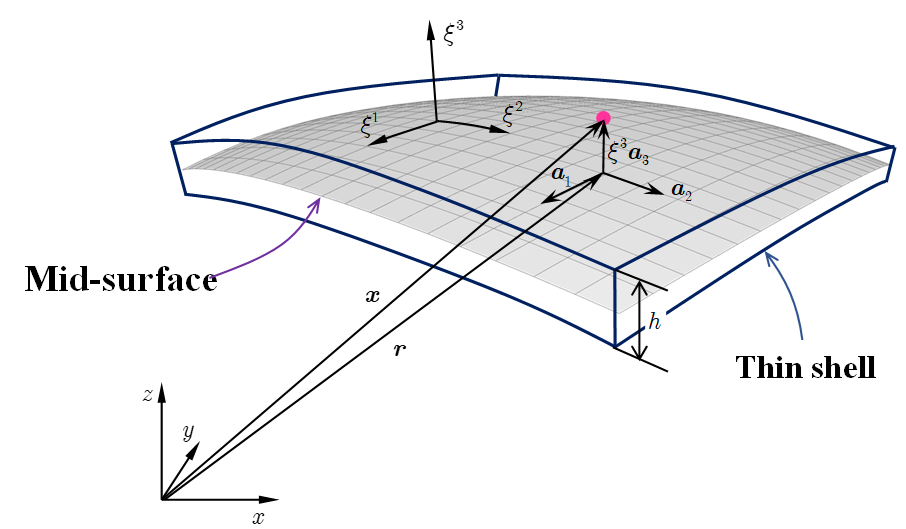
\includegraphics[width=0.7\textwidth]{figures/1}
\caption{Kinematics for thin shell.}\label{fig1}
\end{figure}
in which $\boldsymbol r$ means the position on the mid-surface of shell, and $\boldsymbol a_3$ is corresponding normal direction. For the mid-surface of shell, the in-plane covariant base vector with respect to $\xi^\alpha$ can be derived by a trivial partial differentiation to $\boldsymbol r$:
\begin{equation}
\boldsymbol a_\alpha = \frac{\partial \boldsymbol r}{\partial \xi^\alpha} = \boldsymbol r_{,\alpha}, \alpha  = 1,2
\end{equation}
to provide for a clear expression, the subscript comma denotes the partial differentiation operation with respect to in-plane coordinates $\xi^\alpha$, and the normal vector $\boldsymbol a_3$ can be obtained by the normalized cross product of $\boldsymbol a_{\alpha}$'s as follows:
\begin{equation}
\boldsymbol a_3 = \frac{\boldsymbol a_1 \times \boldsymbol a_2}{\Vert \boldsymbol a_1 \times \boldsymbol a_2 \Vert}
\end{equation}
where $\Vert \bullet \Vert$ is the Euclidean norm operator.

With the assumption of infinitesimal deformation, the strain components with respect to the global contravariant base can be stated as:
\begin{equation}\label{epsilon}
\epsilon_{ij} = \frac{1}{2}(\boldsymbol x_{,i} \cdot \boldsymbol u_{,j} + \boldsymbol u_{,i} \cdot \boldsymbol x_{,j})
\end{equation}
where $\boldsymbol u$ represents the displacement for the shell deformation. To satisfy the Kirchhoff hypothesis, the displacement is assumed to be of the following form:
\begin{equation}\label{u}
\boldsymbol u(\xi^1,\xi^2,\xi^3) = \boldsymbol v(\xi^1,\xi^2) + \boldsymbol \theta(\xi^1,\xi^2) \xi^3
\end{equation}
in which the quadratic and higher order terms are neglected. $\boldsymbol v$, $\boldsymbol \theta$ resperesent the displacement and rotation in mid-surface, respectively.

Subsequently, plugging Eqs. (\ref{x}) and (\ref{u}) into Eq. (\ref{epsilon}) and neglecting the quadratic terms, the strain components can be rephrased as follows:
\begin{subequations}
\begin{align}
\begin{split}
\epsilon_{\alpha\beta} &= \frac{1}{2}(\boldsymbol a_\alpha \cdot \boldsymbol v_{,\beta} + \boldsymbol v_{,\alpha}\cdot \boldsymbol a_\beta) \\ 
&+ \frac{1}{2}(\boldsymbol a_{3,\alpha} \cdot \boldsymbol v_{,\beta} + \boldsymbol v_{,\alpha}\cdot \boldsymbol a_{3,\beta} + \boldsymbol a_\alpha \cdot \boldsymbol \theta_{,\beta} + \boldsymbol \theta_{,\alpha}\cdot \boldsymbol a_\beta)\xi^3 \\
&= \varepsilon_{\alpha\beta} + \kappa_{\alpha\beta}\xi^3
\end{split} \\
\epsilon_{\alpha 3} &= \frac{1}{2}(\boldsymbol a_\alpha \cdot \boldsymbol \theta + \boldsymbol v_{,\alpha}\cdot \boldsymbol a_3) + \frac{1}{2} (\boldsymbol a_3 \cdot \boldsymbol \theta)_{,\alpha}\xi^3 \\ 
\epsilon_{33} &= \boldsymbol a_3 \cdot \boldsymbol \theta
\end{align}
\end{subequations}
where $\varepsilon_{\alpha\beta}$, $\kappa_{\alpha\beta}$ represent membrane and bending strains, respectively, and are given as follows:
\begin{equation}
\varepsilon_{\alpha\beta} = \frac{1}{2}(\boldsymbol a_\alpha \cdot \boldsymbol v_{,\beta} + \boldsymbol v_{,\alpha}\cdot \boldsymbol a_\beta) 
\end{equation}
\begin{equation}\label{kappa1}
\kappa_{\alpha\beta} = \frac{1}{2}(\boldsymbol a_{3,\alpha} \cdot \boldsymbol v_{,\beta} + \boldsymbol v_{,\alpha}\cdot \boldsymbol a_{3,\beta} + \boldsymbol a_\alpha \cdot \boldsymbol \theta_{,\beta} + \boldsymbol \theta_{,\alpha}\cdot \boldsymbol a_\beta)
\end{equation}

In accordance with the Kirchhoff hypothesis, the thickness of shell will not change, and the deformation related with direction of $\xi^3$ will vanish, i.e. $\epsilon_{3i}=0$. Thus, the rotation $\boldsymbol \theta$ can be rewritten as:
\begin{equation}\label{a3}
\epsilon_{3i} = 0 \Rightarrow
\left \{
\begin{split}
&\boldsymbol \theta \cdot \boldsymbol a_\alpha + \boldsymbol v_{,\alpha} \cdot \boldsymbol a_3 = 0 \\
&\boldsymbol \theta \cdot \boldsymbol a_3 = 0
\end{split}
\right .
\Rightarrow \boldsymbol \theta = - \boldsymbol v_{,\alpha} \cdot \boldsymbol a_3 \boldsymbol a^\alpha
\end{equation}
where $\boldsymbol a^\alpha$'s is the in-plane contravariant base vector, $\boldsymbol a^\alpha \cdot \boldsymbol a_\beta = \delta^\alpha_\beta$, $\delta$ is the Kronecker delta function. Substituting Eq. (\ref{a3}) into Eq. (\ref{kappa1}) leads to:
\begin{equation}
\kappa_{\alpha\beta} = (\Gamma^\gamma_{\alpha\beta} \boldsymbol v_{,\gamma} - \boldsymbol v_{,\alpha\beta}) \cdot \boldsymbol a_3 = - \boldsymbol v_{,\alpha}\vert_\beta \cdot \boldsymbol a_3
\end{equation}
in which $\Gamma^\gamma_{\alpha\beta} = \boldsymbol a_{\alpha,\beta} \cdot \boldsymbol a^\gamma$ is namely the Christoffel symbol of the second kind, and $\boldsymbol v_{,\alpha}\vert\beta$ is the in-plane covariant derivative of $\boldsymbol v_{,\alpha}$, i.e. $\boldsymbol v_{,\alpha}\vert_\beta = \Gamma^\gamma_{\alpha\beta}\boldsymbol v_{,\gamma} - \boldsymbol v_{,\alpha\beta}$.

\subsection{Galerkin weak form for Hu-Washizu principle of complementary energy}
In this study, the Hu-Washizu variational principle of complementary energy \cite{dah-wei1985} was adopted for the development of the proposed analytical approach, the corresponding complementary functional, denoted by $\Pi_C$, is listed as follows:
\begin{equation} \label{functionalc}
\begin{split}
&\Pi_C(\varepsilon_{\alpha\beta},\kappa_{\alpha\beta},N^{\alpha\beta},M^{\alpha\beta}) \\
= &\int_\Omega \frac{h}{2}\varepsilon_{\alpha\beta} C^{\alpha\beta\gamma\eta}\varepsilon_{\gamma\eta}d\Omega 
+ \int_\Omega \frac{h^3}{24}\kappa_{\alpha\beta} C^{\alpha\beta\gamma\eta}\kappa_{\gamma\eta}d\Omega \\
+& \int_\Omega \varepsilon_{\alpha\beta} (N^{\alpha\beta} - h C^{\alpha\beta\gamma\eta} \varepsilon_{\gamma\eta}) d\Omega
+ \int_\Omega \kappa_{\alpha\beta} (M^{\alpha\beta} - \frac{h^3}{12} C^{\alpha\beta\gamma\eta} \kappa_{\gamma\eta}) d\Omega \\
-& \int_{\Gamma_v} \boldsymbol T \cdot \bar{\boldsymbol v} d\Gamma 
+ \int_{\Gamma_\theta} M_{\boldsymbol{nn}} \bar \theta_{\boldsymbol n} d\Gamma - (P \boldsymbol a_3 \cdot \bar{\boldsymbol v})_{\boldsymbol x \in C_w} \\
\end{split}
\end{equation}
where $C^{\alpha\beta\gamma\eta}$'s represent the components of fourth order elasticity tensor with respect to the covariant base and plane stress assumption, and it can be expressed by Young's modulus $E$, Poisson's ratio $\nu$ and the in-plane contravariant metric coefficients $a^{\alpha\beta}$'s, $a^{\alpha\beta} = \boldsymbol a^\alpha \cdot \boldsymbol a^\beta$, as follows: 
\begin{equation}
C^{\alpha\beta\gamma\eta} = \frac{E}{2(1+\nu)}(a^{\alpha\gamma}a^{\beta\eta} + a^{\alpha\eta}a^{\beta\gamma} + \frac{2\nu}{1-\nu} a^{\alpha\beta}a^{\gamma\eta})
\end{equation}
and $N^{\alpha\beta}$, $M^{\alpha\beta}$ are the components of membrane and bending stresses given by:
\begin{equation}
N^{\alpha\beta} = hC^{\alpha\beta\gamma\eta}\varepsilon_{\gamma\eta}, \quad
M^{\alpha\beta} = \frac{h^3}{12}C^{\alpha\beta\gamma\eta}\kappa_{\gamma\eta}
\end{equation}

Essential boundaries on the edges and corners denoted by $\Gamma_v$, $\Gamma_\theta$ and $C_v$ are naturally existed in complementary energy functional, $\bar{\boldsymbol v}$, $\bar \theta_{\boldsymbol n}$ are the corresponding prescribed displacement and normal rotation,respectively. $\boldsymbol T$, $M_{\boldsymbol{nn}}$ and $P$ can be determined by Euler-Lagrange equations of shell problem \cite{benzaken2021} as follows:
\begin{equation}
\boldsymbol T = \boldsymbol T_N + \boldsymbol T_M \; \rightarrow
\begin{cases}
\boldsymbol T_N = \boldsymbol a_\alpha N^{\alpha\beta}n_\beta \\
\boldsymbol T_M = (\boldsymbol a_3 M^{\alpha\beta}s_\alpha n_\beta)_{,\gamma} s^\gamma
+ (\boldsymbol a_3 M^{\alpha\beta})\vert_\beta n_\alpha
\end{cases}
\end{equation}
\begin{equation}
M_{\boldsymbol{nn}} = M^{\alpha\beta}n_\alpha n_\beta
\end{equation}
\begin{equation}
P = -[[M^{\alpha\beta}s_\alpha n_\beta]]
\end{equation}
where $\boldsymbol n = n^\alpha \boldsymbol a_\alpha = n_\alpha \boldsymbol a^\alpha$ and $\boldsymbol s = s^\alpha \boldsymbol a_\alpha = s_\alpha \boldsymbol a^\alpha$ are the outward normal and tangent directions on boundaries. $[[f]]$ is the jump operator defined by:
\begin{equation}
[[f]]_{\boldsymbol x = \boldsymbol x_c} = \lim_{\boldsymbol \epsilon\rightarrow \boldsymbol 0+}(f(\boldsymbol x_c + \boldsymbol \epsilon) - f(\boldsymbol x_c - \boldsymbol \epsilon)), \boldsymbol x_c \in \Gamma
\end{equation}
where $f$ is an arbitrary function on $\Gamma$.

Moreover, the natural boundary conditions should be applied by Lagrangian multiplier method with displacement $\boldsymbol v$ regarded as multiplier. Thus, then the new complementary energy functional namely $\Pi$ is given by:
\begin{equation} \label{functional}
\begin{split}
&\Pi(\boldsymbol v, \varepsilon_{\alpha\beta},\kappa_{\alpha\beta},N^{\alpha\beta},M^{\alpha\beta}) \\
=&\Pi_C(\varepsilon_{\alpha\beta},\kappa_{\alpha\beta},N^{\alpha\beta},M^{\alpha\beta})
+ \int_{\Gamma_M} \theta_{\boldsymbol n} (M_{\boldsymbol{nn}} - \bar M_{\boldsymbol{nn}}) d\Gamma \\
- &\int_{\Gamma_T} \boldsymbol v \cdot (\boldsymbol T - \bar{\boldsymbol T})d\Gamma - \boldsymbol v \cdot \boldsymbol a_3 (P - \bar{P})_{\boldsymbol x \in C_P}
- \int_\Omega \boldsymbol v \cdot (\boldsymbol b - \bar{\boldsymbol b}) d\Omega 
\end{split}
\end{equation}
where $\bar{\boldsymbol T}$, $\bar M_{\boldsymbol nn}$ and $\bar P$ are the prescribed traction, bending moment and concentrated force on edges $\Gamma_T$, $\Gamma_M$ and corner $C_P$ respectively. All the boundaries meet the following geometric relationships:
\begin{equation}\label{geo}
\begin{cases}
\Gamma=\Gamma_v \cup \Gamma_T \cup \Gamma_\theta \cup \Gamma_M, \quad C = C_v \cup C_P, \\
\Gamma_v \cap \Gamma_T = \Gamma_\theta \cap \Gamma_M = C_v \cap C_P = \varnothing
\end{cases}
\end{equation}
and $\bar{\boldsymbol b}$ stands for the prescribed body force in $\Omega$, $\boldsymbol b$ also can be written based on Euler-Lagrange equations \cite{benzaken2021} as:
\begin{equation}
\boldsymbol b = \boldsymbol b_N + \boldsymbol b_M \rightarrow
\begin{cases}
\boldsymbol b_N = (\boldsymbol a_\alpha N^{\alpha\beta})\vert_\beta \\
\boldsymbol b_M = (\boldsymbol a_3 M^{\alpha\beta})\vert_{\alpha\beta}
\end{cases}
\end{equation}

Introducing a standard variational argument to Eq. (\ref{functional}), $\delta \Pi=0$, and considering the arbitrariness of virtual variables, $\delta \boldsymbol v$, $\delta \varepsilon_{\alpha\beta}$, $\delta \kappa_{\alpha\beta}$, $N^{\alpha\beta}$, $M^{\alpha\beta}$ lead to the following weak form:
\begin{subequations}
\begin{equation}\label{w1}
- \int_\Omega h \delta \varepsilon_{\alpha\beta} C^{\alpha\beta\gamma\eta}\varepsilon_{\gamma\eta}d\Omega 
+ \int_\Omega \delta \varepsilon_{\alpha\beta} N^{\alpha\beta} d\Omega = 0
\end{equation}
\begin{equation}\label{w2}
- \int_\Omega \frac{h^3}{12} \delta \kappa_{\alpha\beta} C^{\alpha\beta\gamma\eta}\kappa_{\gamma\eta}d\Omega 
+ \int_\Omega \delta \kappa_{\alpha\beta} M^{\alpha\beta} d\Omega = 0
\end{equation}
\begin{multline}\label{w3}
\int_\Omega \delta N^{\alpha\beta} \varepsilon_{\alpha\beta} d\Omega
- \int_\Gamma \delta \boldsymbol T_N \cdot \boldsymbol v d\Gamma 
+ \int_\Omega \delta \boldsymbol b_N \cdot \boldsymbol v d\Omega \\
+ \int_{\Gamma_v} \delta \boldsymbol T_N \cdot \boldsymbol v d\Gamma 
= \int_{\Gamma_v} \delta \boldsymbol T_N \cdot \bar{\boldsymbol v} d\Gamma 
\end{multline}
\begin{multline}\label{w4}
\int_\Omega \delta M^{\alpha\beta} \kappa_{\alpha\beta} d\Omega 
- \int_\Gamma \delta M_{\boldsymbol{nn}} \theta_{\boldsymbol n}d\Gamma
+ \int_\Gamma \delta \boldsymbol T_M \cdot \boldsymbol v d\Gamma
+ (\delta P \boldsymbol a_3 \cdot \boldsymbol v)_{\boldsymbol x \in C}
+ \int_\Omega \delta \boldsymbol b_M \cdot \boldsymbol v d\Omega \\
+ \int_{\Gamma_\theta} \delta M_{\boldsymbol{nn}} \theta_{\boldsymbol n}d\Gamma
- \int_{\Gamma_v} \delta \boldsymbol T_M \cdot \boldsymbol v d\Gamma
- (\delta P \boldsymbol a_3 \cdot \boldsymbol v)_{\boldsymbol x \in C_v} \\ =
\int_{\Gamma_\theta} \delta M_{\boldsymbol{nn}} \bar{\theta}_{\boldsymbol n}d\Gamma
- \int_{\Gamma_v} \delta \boldsymbol T_M \cdot \bar{\boldsymbol v} d\Gamma
- (\delta P \boldsymbol a_3 \cdot \bar{\boldsymbol v})_{\boldsymbol x \in C_v}
\end{multline}
\begin{multline}\label{w5}
\int_{\Gamma} \delta \theta_{\boldsymbol n} M_{\boldsymbol{nn}} d\Gamma
    - \int_\Gamma \delta \boldsymbol v \cdot \boldsymbol T d\Gamma 
    - (\delta \boldsymbol v \cdot \boldsymbol a_3 P)_{\boldsymbol x \in C}
    + \int_\Omega \delta \boldsymbol v \cdot \boldsymbol b d\Omega \\
    - \int_{\Gamma_\theta} \delta \theta_{\boldsymbol n} M_{\boldsymbol{nn}} d\Gamma
    + \int_{\Gamma_v} \delta \boldsymbol v \cdot \boldsymbol T d\Gamma 
    + (\delta \boldsymbol v \cdot \boldsymbol a_3 P)_{\boldsymbol x \in C_v}
    = - \int_{\Gamma_T} \delta \boldsymbol v \cdot \bar{\boldsymbol t} d\Gamma - \int_\Omega \delta \boldsymbol v \cdot \bar{\boldsymbol b} d\Omega
\end{multline}
\end{subequations}
where the geometric relationships of Eq. (\ref{geo}) is used herein.

%DIFDELCMD < \section{Mixed meshfree formulation for modified Hellinger-Reissner weak form}\label{mixed}
\subsection{Reproducing kernel approximation for displacement}
This study approximates the displacement by adopting reproducing kernel approximation. As shown in Fig. \ref{fig2}, the mid-surface of the shell $\Omega$ is discretized by a set of meshfree nodes $\{\boldsymbol \xi_I\}_{I=1}^{n_p}$ in parametric configuration, where $n_p$ is the total number of meshfree nodes. The approximated displacement namely $\boldsymbol v^h$ can be expressed as:
\begin{equation}\label{approxv}
\boldsymbol v(\boldsymbol \xi) = \sum_{I=1}^{n_p} \Psi_I(\boldsymbol \xi) \boldsymbol d_I
\end{equation}
in which $\Psi_I$ and $\boldsymbol d_I$ is the shape function and nodal coefficient tensor related by node $\boldsymbol \xi_I$. According to reproducing kernel approximation \cite{liu1995}, the shape function takes the following form:
\begin{equation}
\Psi_I(\boldsymbol \xi) = \boldsymbol p^T(\boldsymbol \xi) \boldsymbol c(\boldsymbol \xi) \phi(\boldsymbol \xi_I - \boldsymbol \xi)
\end{equation}
where $\boldsymbol p$ is the basis function vector represented using the following quadratic function as:
\begin{equation}
        \boldsymbol p = \{1,\;\xi^1,\;\xi^2,\;(\xi^1)^2,\xi^1\xi^2,(\xi^2)^2\}^T
\end{equation}

The kernel function denoted by $\phi$ controls the support and smoothness of meshfree shape functions. The quintic B-spline function with square support is used herein as the kernel function:
\begin{equation}
\phi(\boldsymbol \xi_I - \boldsymbol \xi) = \phi(\hat s_1)\phi(\hat s_2), \quad \hat s_\alpha = \frac{\vert \xi^\alpha_I - \xi^\alpha\vert}{s_{\alpha I}}
\end{equation}
with
\begin{equation}
\phi(\hat s_\alpha) = \frac{1}{5!}\begin{cases}
(3-3\hat s_\alpha)^5 - 6(2-3\hat s_\alpha)^5 + 15(1-3\hat s_\alpha)^5 & \hat s_\alpha \le \frac{1}{3} \\
(3-3\hat s_\alpha)^5 - 6(2-3\hat s_\alpha)^5 & \frac{1}{3}<\hat s_\alpha \le \frac{2}{3} \\
(3-3\hat s_\alpha)^5 & \frac{2}{3}<\hat s_\alpha \le 1 \\
0 & \hat s_\alpha >1
\end{cases}
\end{equation}
and $\hat s_{\alpha I}$ means the characterized size of support for meshfree shape function $\Psi_I$.

The unknown vector $\boldsymbol c$ in shape function are determined by the fulfillment of the so-called consistency condition:
\begin{equation}
\sum_{I=1}^{n_p} \Psi_I(\boldsymbol \xi)\boldsymbol p(\boldsymbol \xi_I) = \boldsymbol p(\boldsymbol \xi)
\end{equation}
or equivalently
\begin{equation}\label{cc}
\sum_{I=1}^{n_p} \Psi_I(\boldsymbol \xi)\boldsymbol p(\boldsymbol \xi_I-\boldsymbol \xi) = \boldsymbol p(\boldsymbol 0)
\end{equation}
Substituting Eq. (\ref{approxv}) into (\ref{cc}), yields:
\begin{equation}\label{A}
\boldsymbol A(\boldsymbol \xi) \boldsymbol c(\boldsymbol \xi) = \boldsymbol p(\boldsymbol 0)\quad \Rightarrow \quad
\boldsymbol c(\boldsymbol \xi) = \boldsymbol A^{-1}(\boldsymbol \xi)\boldsymbol p(\boldsymbol 0)
\end{equation}
where $\boldsymbol A$ is the moment matrix:
\begin{equation}
\boldsymbol A(\boldsymbol \xi) = \sum_{I=1}^{n_p}\phi(\boldsymbol \xi_I - \boldsymbol \xi) \boldsymbol p(\boldsymbol \xi_I-\boldsymbol \xi)\boldsymbol p^T(\boldsymbol \xi_I - \boldsymbol \xi)
\end{equation}
Substituting Eq. (\ref{A}) back into Eq. (\ref{approxv}), the expression of meshfree shape function can be written as:
\begin{equation}
\Psi_I(\boldsymbol \xi) = \boldsymbol p^T(\boldsymbol \xi_I - \boldsymbol \xi)\boldsymbol A^{-1}(\boldsymbol \xi) \boldsymbol p(\boldsymbol 0) \phi(\boldsymbol \xi_I-\boldsymbol \xi)
\end{equation}
\subsection{Reproducing kernel gradient smoothing approximation for effective stress and strain}
In Galerkin meshfree formulation, the mid-plane of thin shell $\Omega$ is split by a set of integration cells $\Omega_C$'s, $\cup_{C=1}^{n_e}\Omega_C\approx \Omega$, as shown in Fig. \ref{fig2}. With the inspiration of reproducing kernel smoothing framework, the Cartesian and covariant derivatives of displacement, $\boldsymbol v_{,\alpha}$ and $-\boldsymbol v_{,\alpha}\vert_\beta$, in strains $\varepsilon_{\alpha\beta}$, $\kappa_{\alpha\beta}$ are approximated by $(p-1)$-th order polynomials in each integration cells. In integration cell $\Omega_C$, the approximated derivatives and strains denoted by $\boldsymbol v^h_{,\alpha}$, $\varepsilon^h_{\alpha\beta}$ and $-\boldsymbol v^h_{,\alpha}\vert_\beta$, $\kappa^h_{\alpha\beta}$ can be expressed by:
\begin{equation}\label{approxsn1}
    \boldsymbol v^h_{,\alpha}(\boldsymbol \xi) = \boldsymbol q^T(\boldsymbol \xi) \boldsymbol d_{\alpha}^\varepsilon, \quad
    \varepsilon^h_{\alpha\beta}(\boldsymbol \xi) = \boldsymbol q^T(\boldsymbol \xi) \frac{1}{2}(\boldsymbol a_\alpha \cdot \boldsymbol d_{\beta}^\varepsilon + \boldsymbol a_\beta \cdot \boldsymbol d_{\alpha}^\varepsilon)
\end{equation}
\begin{equation}\label{approxsn2}
    -\boldsymbol v^h_{,\alpha}\vert_\beta(\boldsymbol \xi) = \boldsymbol q^T(\boldsymbol \xi) \boldsymbol d_{\alpha\beta}^\kappa , \quad
    \kappa^h_{\alpha\beta}(\boldsymbol \xi) = \boldsymbol q^T(\boldsymbol \xi) \boldsymbol a_3 \cdot \boldsymbol d_{\alpha\beta}^\kappa
\end{equation}
where $\boldsymbol q$ is the linear polynomial vector and has the following form:
\begin{equation}
\boldsymbol q = \{ 1,\; \xi^1,\; \xi^2\}^T
\end{equation}
and the $\boldsymbol d^\varepsilon_{\alpha}$, $\boldsymbol d^\kappa_{\alpha\beta}$ are the corresponding coefficient vector tensors. For the conciseness, the mixed usage of tensor and vector is introduced in this study. For instance, the component of coefficient tensor vector $\boldsymbol d^\varepsilon_{\alpha I}$, $\boldsymbol d^\varepsilon_\alpha = \{\boldsymbol d^\varepsilon_{\alpha I}\}$, is a three dimensional tensor, $\dim \boldsymbol d^\varepsilon_{\alpha I} = \dim \boldsymbol v$.

\begin{figure}[!ht]
\centering
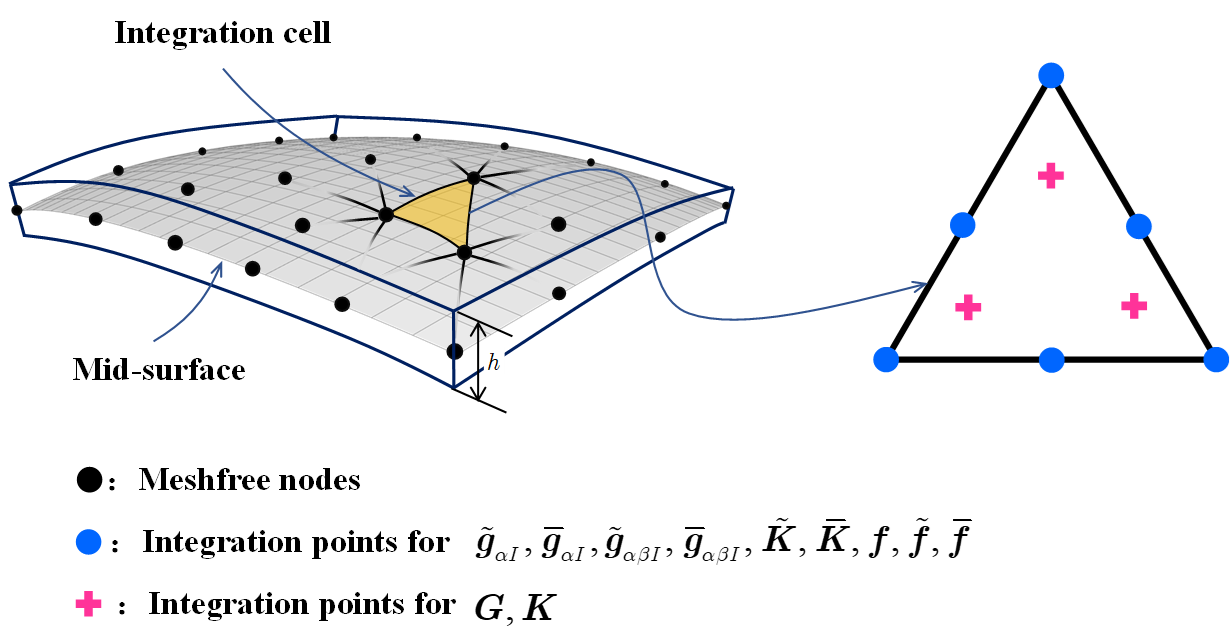
\includegraphics[width=\textwidth]{figures/2}
\caption{Integration scheme for Hu-Washizu weak form.}\label{fig2}
\end{figure}

In order to meet the integration constraint of thin shell problem, the approximated stresses $N^{\alpha\beta h}$, $M^{\alpha\beta h}$ are assumed to be a similar form with strains, yields:
\begin{equation}\label{approxse1}
N^{\alpha\beta h}(\boldsymbol \xi) = \boldsymbol q^T(\boldsymbol \xi) \boldsymbol a^\alpha \cdot \boldsymbol d^{\beta}_N,\quad
\boldsymbol a_\alpha N^{\alpha\beta h}(\boldsymbol \xi) = \boldsymbol q^T(\boldsymbol \xi) \boldsymbol d_N^\beta
\end{equation}
\begin{equation}\label{approxse2}
    M^{\alpha\beta h}(\boldsymbol \xi) = \boldsymbol q^T(\boldsymbol \xi) \boldsymbol a_3 \cdot \boldsymbol d^{\alpha\beta}_M,\quad
    \boldsymbol a_3 M^{\alpha\beta h}(\boldsymbol \xi) = \boldsymbol q^T(\boldsymbol \xi) \boldsymbol d^{\alpha\beta}_M
\end{equation}
substituting the approximations of Eqs. (\ref{approxv}), (\ref{approxsn1}), (\ref{approxsn2}), (\ref{approxse1}), (\ref{approxse2}) into Eqs. (\ref{w3}), (\ref{w4}) can express $\boldsymbol d^\varepsilon_\beta$ and $\boldsymbol d^\kappa_{\alpha\beta}$ by $\boldsymbol d$ as:
\begin{equation}\label{depsilon}
\boldsymbol d^\varepsilon_\beta = \boldsymbol G^{-1} \left (\sum_{I=1}^{n_p}(\tilde{\boldsymbol g}_{\beta I} - \bar{\boldsymbol g}_{\beta I}) \boldsymbol d_I + \hat{\boldsymbol g}_\beta \right )
\end{equation}
\begin{equation}\label{dkappa}
\boldsymbol d^\kappa_{\alpha\beta} = \boldsymbol G^{-1} \left (\sum_{I=1}^{n_p}(\tilde{\boldsymbol g}_{\alpha\beta I} - \bar{\boldsymbol g}_{\alpha\beta I})\boldsymbol d_I + \hat{\boldsymbol g}_{\alpha\beta} \right )
\end{equation}
with
\begin{equation}
\boldsymbol G = \int_{\Omega_C} \boldsymbol q^T \boldsymbol q d\Omega
\end{equation}
\begin{subequations}\label{gn}
\begin{align}
\tilde{\boldsymbol g}_{\beta I} &= \int_{\Gamma_C} \Psi_I \boldsymbol q n_\beta d\Gamma
- \int_{\Omega_C} \Psi_I \boldsymbol q_{\vert \beta} d\Omega \\
\bar{\boldsymbol g}_{\beta I} &= \int_{\Gamma_C\cap\Gamma_v} \Psi_I \boldsymbol q n_\beta d\Gamma \\
\hat{\boldsymbol g}_{\beta} &= \int_{\Gamma_C\cap\Gamma_v} \boldsymbol q n_\beta \bar{\boldsymbol v} d\Gamma 
\end{align}
\end{subequations}
\begin{subequations}\label{gm}
\begin{align}
\small
\begin{split}
\tilde{\boldsymbol g}_{\alpha\beta I} &= \int_{\Gamma_C} \Psi_{I,\gamma}n^\gamma \boldsymbol q n_\alpha n_\beta d\Gamma 
- \int_{\Gamma_C} \Psi_I(\boldsymbol q_{\vert \beta} n_\alpha + (\boldsymbol q s_\alpha n_\beta)_{,\gamma}s^\gamma) d\Gamma \\
&+ [[\Psi_I \boldsymbol q s_\alpha n_\beta]]_{\boldsymbol x\in C_C}
- \int_{\Omega_C} \Psi \boldsymbol q_{,\alpha\vert \beta} d\Omega \\
\end{split} \\
\small
\begin{split}
\bar{\boldsymbol g}_{\alpha\beta I} &= \int_{\Gamma_C\cap\Gamma_\theta} \Psi_{I,\gamma}n^\gamma \boldsymbol q n_\alpha n_\beta d\Gamma 
- \int_{\Gamma_C\cap\Gamma_v} \Psi_I(\boldsymbol q_{\vert \beta} n_\alpha + (\boldsymbol q s_\alpha n_\beta)_{,\gamma}s^\gamma) d\Gamma \\
&+ [[\Psi_I \boldsymbol q s_\alpha n_\beta]]_{\boldsymbol x\in C_C\cap C_v}
\end{split} \\
\small
\begin{split}
\hat{\boldsymbol g}_{\alpha\beta} &= \int_{\Gamma_C\cap\Gamma_\theta} \boldsymbol q n_\alpha n_\beta \boldsymbol a_3 \bar{\theta}_{\boldsymbol n} d\Gamma 
- \int_{\Gamma_C\cap\Gamma_v}(\boldsymbol q_{\vert \beta} n_\alpha + (\boldsymbol q s_\alpha n_\beta)_{,\gamma}s^\gamma)\bar{\boldsymbol v} d\Gamma \\
&+ [[\boldsymbol q s_\alpha n_\beta \bar{\boldsymbol v}]]_{\boldsymbol x\in C_C\cap C_v}
\end{split}
\end{align}
\end{subequations}
where evaluations of $\boldsymbol q_{\vert \beta}$, $\boldsymbol q_{,\alpha\vert\beta}$ are detail in \ref{derivative}. Further plugging Eqs. (\ref{depsilon}) and (\ref{dkappa}) back into Eqs. (\ref{approxsn1}) and (\ref{approxsn2}) respectively gives the final expression of $\boldsymbol v^h_{,\alpha}$, $\varepsilon^h_{\alpha\beta}$ and $-\boldsymbol v^h_{,\alpha\beta}$, $\boldsymbol \kappa^h_{\alpha\beta}$ as: \begin{subequations}
\begin{equation}
\boldsymbol v^h_{,\alpha} = \sum_{I=1}^{n_p}(
\tilde \Psi_{I,\alpha} - \bar \Psi_{I,\alpha}) \boldsymbol d_I +
\boldsymbol q^T \boldsymbol G^{-1}\hat{\boldsymbol g}_{\alpha}
\end{equation}
\begin{equation}\label{epsilonh}
\begin{split}
\varepsilon^h_{\alpha\beta} &= 
\sum_{I=1}^{n_p} \frac{1}{2}(\boldsymbol a_\alpha \tilde \Psi_{I,\beta} + \boldsymbol a_\beta \tilde \Psi_{I,\alpha}) \cdot \boldsymbol d_I 
- \sum_{I=1}^{n_p} \frac{1}{2}(\boldsymbol a_\alpha \bar \Psi_{I,\beta} + \boldsymbol a_\beta \bar \Psi_{I,\alpha}) \cdot \boldsymbol d_I \\
&+ \boldsymbol q^T \boldsymbol G^{-1} \frac{1}{2}(\boldsymbol a_\alpha \cdot \hat{\boldsymbol g}_{\beta} + \boldsymbol a_\beta \cdot \hat{\boldsymbol g}_{\alpha}) \\
&= \tilde \varepsilon^h_{\alpha\beta} - \bar \varepsilon^h_{\alpha\beta} + \hat \varepsilon^h_{\alpha\beta}
\end{split}
\end{equation}
\end{subequations}
\begin{subequations}
\begin{equation}
-\boldsymbol v^h_{,\alpha}\vert_\beta = \sum_{I=1}^{n_p} (
\tilde \Psi_{I,\alpha\beta} -
\bar \Psi_{I,\alpha\beta} ) \boldsymbol d_I +
\boldsymbol q^T \boldsymbol G^{-1}\hat{\boldsymbol g}_{\alpha\beta}
\end{equation}
\begin{equation}\label{kappah}
\begin{split}
\kappa^h_{\alpha\beta} &= \sum_{I=1}^{n_p} \tilde \Psi_{I,\alpha\beta} \boldsymbol a_3 \cdot \boldsymbol d_I
- \sum_{I=1}^{n_p} \bar \Psi_{I,\alpha\beta} \boldsymbol a_3 \cdot \boldsymbol d_I +
\boldsymbol q^T \boldsymbol G^{-1}\boldsymbol a_3 \cdot \hat{\boldsymbol g}_{\alpha\beta} \\
&= \tilde \kappa^h_{\alpha\beta} - \bar \kappa^h_{\alpha\beta} + \hat \kappa^h_{\alpha\beta}
\end{split}
\end{equation}
\end{subequations}
with
\begin{equation}\label{epsilon2}
\left \{
\begin{split}
\tilde \varepsilon^h_{\alpha\beta} &= \sum_{I=1}^{n_p} \frac{1}{2}(\boldsymbol a_\alpha \tilde \Psi_{I,\beta} + \boldsymbol a_\beta \tilde \Psi_{I,\alpha}) \cdot \boldsymbol d_I
=\sum_{I=1}^{n_p} \tilde{\boldsymbol \varepsilon}_{\alpha\beta I} \cdot \boldsymbol d_I \\
\bar \varepsilon^h_{\alpha\beta} &= \sum_{I=1}^{n_p} \frac{1}{2}(\boldsymbol a_\alpha \bar \Psi_{I,\beta} + \boldsymbol a_\beta \bar \Psi_{I,\alpha}) \cdot \boldsymbol d_I
=\sum_{I=1}^{n_p} \bar{\boldsymbol \varepsilon}_{\alpha\beta I} \cdot \boldsymbol d_I \\
\hat \varepsilon^h_{\alpha\beta} &= \boldsymbol q^T \boldsymbol G^{-1} \frac{1}{2}(\boldsymbol a_\alpha\cdot\hat{\boldsymbol g}_\beta + \boldsymbol a_\beta \cdot \hat{\boldsymbol g}_\alpha)
\end{split}
\right .
\end{equation}
\begin{equation}
\left \{
\begin{split}
&\tilde{\Psi}_{I,\alpha}(\boldsymbol \xi) = \boldsymbol q^T(\boldsymbol \xi) \boldsymbol G^{-1} \tilde{\boldsymbol g}_{\alpha I} \\
&\bar{\Psi}_{I,\alpha}(\boldsymbol \xi) = \boldsymbol q^T(\boldsymbol \xi) \boldsymbol G^{-1} \bar{\boldsymbol g}_{\alpha I} \\
&\tilde{\boldsymbol \varepsilon}_{\alpha\beta I} = \frac{1}{2}(\boldsymbol a_\alpha \tilde \Psi_{I,\beta} + \boldsymbol a_\beta \tilde \Psi_{I,\alpha}) \\
&\bar{\boldsymbol \varepsilon}_{\alpha\beta I} = \frac{1}{2}(\boldsymbol a_\alpha \bar \Psi_{I,\beta} + \boldsymbol a_\beta \bar \Psi_{I,\alpha})
\end{split}
\right .
\end{equation}
\begin{equation}\label{kappa2}
\left \{
\begin{split}
\tilde \kappa^h_{\alpha\beta} &= \sum_{I=1}^{n_p} \tilde \Psi_{I,\alpha\beta}\boldsymbol a_3 \cdot \boldsymbol d_I 
= \sum_{I = 1}^{n_p} \tilde{\boldsymbol \kappa}_{\alpha\beta I} \cdot \boldsymbol d_I\\
\bar \kappa^h_{\alpha\beta} &= \sum_{I=1}^{n_p} \bar \Psi_{I,\alpha\beta}\boldsymbol a_3 \cdot \boldsymbol d_I
= \sum_{I = 1}^{n_p} \bar{\boldsymbol \kappa}_{\alpha\beta I} \cdot \boldsymbol d_I \\
\hat \kappa^h_{\alpha\beta} &= \boldsymbol q^T \boldsymbol G^{-1} \boldsymbol a_3 \cdot \hat{\boldsymbol g}_{\alpha\beta}
\end{split}
\right .
\end{equation}
\begin{equation}
\left \{
\begin{split}
&\tilde{\Psi}_{I,\alpha\beta}(\boldsymbol \xi) = \boldsymbol q^T(\boldsymbol \xi) \boldsymbol G^{-1} \tilde{\boldsymbol g}_{\alpha\beta I} \\
&\bar{\Psi}_{I,\alpha\beta}(\boldsymbol \xi) = \boldsymbol q^T(\boldsymbol \xi) \boldsymbol G^{-1} \tilde{\boldsymbol g}_{\alpha\beta I} \\
&\tilde{\boldsymbol \kappa}_{\alpha\beta I} = \tilde \Psi_{I,\alpha\beta}\boldsymbol a_3 \\
&\bar {\boldsymbol \kappa}_{\alpha\beta I} = \bar \Psi_{I,\alpha\beta}\boldsymbol a_3 \\
\end{split}
\right .
\end{equation}

% Furthermore, taking Eqs. (\ref{approxsn1}) and (\ref{approxsn2}) into Eqs.(\ref{w1}) and (\ref{w2}) can obtain the approximated effective stresses $N^{\alpha\beta h}$, $M^{\alpha\beta h}$ and their coefficients $\boldsymbol d_N^\beta$, $\boldsymbol d_M^{\alpha\beta}$ as:
% \begin{equation}\label{d_N1}
%  \delta \boldsymbol d^\varepsilon_\alpha \cdot \boldsymbol G^{\alpha\eta}_N \cdot \boldsymbol d^\varepsilon_\eta = \delta \boldsymbol d^\varepsilon_\alpha \cdot \boldsymbol d_N^\alpha \boldsymbol G \quad\Rightarrow \quad & \boldsymbol d_N^\alpha = \boldsymbol G^{-1} \boldsymbol G_N^{\alpha\eta} \cdot \boldsymbol d^\varepsilon_\eta
% \end{equation}
% \begin{equation}\label{d_M1}
%  \delta \boldsymbol d^\kappa_{\alpha\beta} : \boldsymbol G_M^{\alpha\beta\gamma\eta} : \boldsymbol d^\kappa_{\gamma\eta} \boldsymbol G = \delta \boldsymbol d^\kappa_{\alpha\beta} \cdot \boldsymbol d_M^{\alpha\beta} \boldsymbol G \\
% \Rightarrow \; \boldsymbol d_M^{\alpha\beta} = \boldsymbol G^{-1} \boldsymbol G_{\alpha\beta}^M \cdot \boldsymbol d^\kappa_{\gamma\eta}
% \end{equation}
% with
% \begin{equation}
% \boldsymbol G^{\alpha\eta}_N = \int_{\Omega_C} \boldsymbol a_\beta hC^{\alpha\beta\gamma\eta} \boldsymbol a_\gamma \boldsymbol q \boldsymbol q^T d\Omega
% \end{equation}
% \begin{equation}
% \boldsymbol G^{\alpha\beta\gamma\eta}_M = \int_{\Omega_C} \boldsymbol a_3 \frac{h^3}{12}C^{\alpha\beta\gamma\eta}\boldsymbol a_3 \boldsymbol q\boldsymbol q^T d\Omega
% \end{equation}
%  
% Finally, taking Eqs. (\ref{d_N1}) and (\ref{d_M1}) back to Eqs. (\ref{approxse1}), (\ref{approxse2}) can express the components of stresses as follows:
% \begin{equation}\label{Nh}
% N^{\alpha\beta h} = \boldsymbol q^T \boldsymbol G^{-1}\frac{1}{2}(\boldsymbol a^\alpha \cdot \boldsymbol G^{\beta\gamma}_{N} + \boldsymbol a^\beta \cdot \boldsymbol G^{\alpha\gamma}_N) \cdot \boldsymbol d^{\varepsilon}_\gamma
% \end{equation}
% \begin{equation}\label{Mh}
% M^{\alpha\beta h} = \boldsymbol q^T \boldsymbol G^{-1} \boldsymbol a_3 \cdot \boldsymbol G^{\alpha\beta\gamma\eta}_M \cdot \boldsymbol d^\kappa_{\gamma\eta}
% \end{equation}

It has to be noted that, referring to reproducing kernel gradient smoothing framework \cite{wang2019a}, $\tilde \Psi_{I,\alpha}$, $\tilde \Psi_{I,\alpha\beta}$ are actually the first and second order smoothed gradients in curvilinear coordinates. $\tilde{\boldsymbol g}_{\alpha I}$ and $\tilde{\boldsymbol g}_{\alpha \beta I}$ are the right hand side integration constraints for first and second order gradients, then this formulation can meet the variational consistency for the $p$-th order polynomials. It should be known that, in curved model, the variational consistency for non-polynomial functions, like trigonometric functions, should be required for the polynomial solution. Even with $p$-th order variational consistency, the proposed formulation can not exactly reproduce the solution spanned by basis functions. However, the accuracy of reproducing kernel smoothed gradients is still better that traditional meshfree formulation. Numerical examples in the section below will provide better evidence to prove the accuracy of the reproducing kernel smoothed gradients.


%DIFDELCMD < \section{Naturally variational enforcement for essential boundary conditions}\label{boundary}
\subsection{Discrete equilibrium equations}
With the approximated effective stresses and strains, the last equation of weak form Eq. (\ref{w5}) becomes:
\begin{equation}\label{w51}
- \sum_{C=1}^{n_e}\sum_{I=1}^{n_p} \delta \boldsymbol d_I \cdot \left ( (\tilde{\boldsymbol g}^T_{\alpha I} - \bar{\boldsymbol g}^T_{\alpha I}) \boldsymbol d_N^{\alpha}
+ (\tilde{\boldsymbol g}^T_{\alpha\beta I} - \bar{\boldsymbol g}^T_{\alpha\beta I}) \boldsymbol d_M^{\alpha\beta} \right ) = - \sum_{I=1}^{n_p}\delta d_I \cdot \boldsymbol f_I
\end{equation}
where $\boldsymbol f_I$'s are the components of the traditional force vector:
\begin{equation}
        \boldsymbol f_I = \int_{\Gamma_t} \Psi_I \bar{\boldsymbol t} d\Gamma - \int_{\Gamma_M} \Psi_{I,\gamma} n^\gamma \bar M_{\boldsymbol{nn}} d\Gamma + [[\Psi_I\boldsymbol a_3 \bar P]]_{\boldsymbol x\in C_P} + \int_\Omega \Psi_I \bar{\boldsymbol b} d\Omega
\end{equation}
The left side of Eq. (\ref{w51}) can be simplified using the following steps. For clarity, the derivation of first term in Eq. (\ref{w51}) taken as an example is given by:
\begin{equation}
\begin{split}
\sum_{I=1}^{n_p} \delta \boldsymbol d_I \cdot \tilde{\boldsymbol g}^T_{\alpha I} \boldsymbol d_N^\alpha 
&= \sum_{I=1}^{n_p} \delta \boldsymbol d_I \cdot (\boldsymbol G^{-1} \tilde{\boldsymbol g}_{\alpha I})^T  \boldsymbol G \boldsymbol d^\alpha_N \\
&= \int_{\Omega_C} \sum_{I=1}^{n_p} \delta \boldsymbol d_I \cdot (\boldsymbol q^T\boldsymbol G^{-1} \tilde{\boldsymbol g}_{\alpha I})^T  \boldsymbol q^T \boldsymbol d^\alpha_N d\Omega \\
&= \int_{\Omega_C} \sum_{I=1}^{n_p} \delta \boldsymbol d_I \cdot \boldsymbol a_\beta(\boldsymbol q^T\boldsymbol G^{-1} \tilde{\boldsymbol g}_{\alpha I})^T  N^{\alpha\beta h} d\Omega \\
& = \int_{\Omega_C} \delta \tilde \varepsilon_{\alpha\beta}^h N^{\alpha\beta h} d\Omega 
\end{split}
\end{equation}
following the above procedure and including the weak form of Eqs. (\ref{w1}), (\ref{w2}), the left side of Eq. (\ref{w51}) in $\Omega_C$ becomes:
\begin{equation}
\begin{split}
&\sum_{I=1}^{n_p} \delta \boldsymbol d_I \cdot  \left ( 
(\tilde{\boldsymbol g}^T_{\alpha I} - \bar{\boldsymbol g}^T_{\alpha I}) \boldsymbol d^\alpha_N
+(\tilde{\boldsymbol g}^T_{\alpha\beta I} - \bar{\boldsymbol g}^T_{\alpha\beta I}) \boldsymbol d^{\alpha\beta}_M \right) \\
=& \int_{\Omega_C}\left ( (\delta \tilde \varepsilon^h_{\alpha\beta} - \delta \bar \varepsilon^h_{\alpha\beta}) N^{\alpha\beta h}
+ (\delta \tilde \kappa^h_{\alpha\beta} - \delta \bar \kappa^h_{\alpha\beta})M^{\alpha\beta h}
\right ) d\Omega \\
= &\int_{\Omega_C} (\delta \tilde \varepsilon^h_{\alpha\beta} - \delta \bar \varepsilon^h_{\alpha\beta}) hC^{\alpha\beta\gamma\eta} \varepsilon^h_{\gamma\eta}
+ (\delta \tilde \kappa^h_{\alpha\beta} - \delta \bar \kappa^h_{\alpha\beta}) \frac{h^3}{12}C^{\alpha\beta\gamma\eta}\kappa^h_{\gamma\eta} \\
= &\int_{\Omega_C}\delta \tilde \varepsilon^h_{\alpha\beta}hC^{\alpha\beta\gamma\eta} \tilde\varepsilon^h_{\gamma\eta} d\Omega
+ \int_{\Omega_C}\delta \tilde \kappa^h_{\alpha\beta} \frac{h^3}{12}C^{\alpha\beta\gamma\eta}\tilde \kappa^h_{\gamma\eta}d\Omega \\
- &\int_{\Omega_C}\delta \tilde \varepsilon^h_{\alpha\beta}hC^{\alpha\beta\gamma\eta} \bar \varepsilon^h_{\gamma\eta} d\Omega
- \int_{\Omega_C}\delta \bar \varepsilon^h_{\alpha\beta}hC^{\alpha\beta\gamma\eta} \tilde \varepsilon^h_{\gamma\eta} d\Omega \\
- &\int_{\Omega_C}\delta \tilde \kappa^h_{\alpha\beta} \frac{h^3}{12}C^{\alpha\beta\gamma\eta}\bar \kappa^h_{\gamma\eta}d\Omega 
- \int_{\Omega_C}\delta \bar \kappa^h_{\alpha\beta} \frac{h^3}{12}C^{\alpha\beta\gamma\eta}\tilde \kappa^h_{\gamma\eta}d\Omega \\
+ &\int_{\Omega_C}\delta \bar \varepsilon^h_{\alpha\beta}hC^{\alpha\beta\gamma\eta} \bar \varepsilon^h_{\gamma\eta} d\Omega
+ \int_{\Omega_C}\delta \bar \kappa^h_{\alpha\beta} \frac{h^3}{12}C^{\alpha\beta\gamma\eta}\bar \kappa^h_{\gamma\eta}d\Omega \\
+ &\int_{\Omega_C}(\delta \tilde \varepsilon^h_{\alpha\beta} - \delta \bar \varepsilon^h_{\alpha\beta})hC^{\alpha\beta\gamma\eta} \hat \varepsilon^h_{\gamma\eta} d\Omega
+ \int_{\Omega_C}(\delta \tilde \kappa^h_{\alpha\beta} - \delta \bar \kappa^h_{\alpha\beta})\frac{h^3}{12}C^{\alpha\beta\gamma\eta}\hat \kappa^h_{\gamma\eta}d\Omega \\
\end{split}
\end{equation}
on further substituting Eqs. (\ref{epsilon2}) and (\ref{kappa2}) into above equation gives the final discrete equilibrium equations, respectively: 
\begin{equation}
        (\boldsymbol K + \tilde{\boldsymbol K} + \bar{\boldsymbol K} )\boldsymbol d = \boldsymbol f + \tilde{\boldsymbol f} + \bar{\boldsymbol f}
\end{equation}
where
\begin{equation}\label{de1}
        \boldsymbol K_{IJ} = \int_\Omega \tilde{\boldsymbol \varepsilon}_{\alpha\beta I} hC^{\alpha\beta\gamma\eta}\tilde{\boldsymbol \varepsilon}_{\gamma\eta J} d\Omega + \int_\Omega \tilde{\boldsymbol \kappa}_{\alpha\beta I} \frac{h^3}{12}C^{\alpha\beta\gamma\eta} \tilde{\boldsymbol \kappa}_{\alpha\beta J} d\Omega
\end{equation}
\begin{subequations}\label{de2}
\begin{align}
\begin{split}
        \tilde{\boldsymbol K}_{IJ} = &- \int_{\Gamma_v} (\Psi_I \tilde{\boldsymbol T}_{NJ} + \tilde{\boldsymbol T}_{NJ} \Psi_J) d\Gamma \\
                                     &+ \int_{\Gamma_\theta} (\Psi_{I,\gamma} n^\gamma \boldsymbol a_3 \tilde{\boldsymbol M}_{\boldsymbol{nn}J} + \boldsymbol a_3 \tilde{\boldsymbol M}_{\boldsymbol{nn}I} \Psi_{I,\gamma}n^\gamma)d\Gamma \\
                                     & + ([[\Psi_I \boldsymbol a_3 \tilde{\boldsymbol P}_J]] + [[\tilde{\boldsymbol P}_I \boldsymbol a_3 \Psi_J]])_{\boldsymbol x \in C_v}
\end{split} \\
\tilde{\boldsymbol f}_I = &- \int_{\Gamma_v} \tilde{\boldsymbol T}_{NI} \cdot \bar{\boldsymbol v} d\Gamma + \int_{\Gamma_\theta} \tilde{\boldsymbol M}_{\boldsymbol{nn}I} \bar{\theta}_{\boldsymbol n} d\Gamma + [[\tilde{\boldsymbol P}_I\boldsymbol a_3 \cdot \bar{\boldsymbol v}]]_{\boldsymbol x \in C_v}
\end{align}
\end{subequations}
\begin{subequations}\label{de3}
\begin{align}
\bar{\boldsymbol K}_{IJ} &= - \int_{\Gamma_v} \bar{\boldsymbol T}_{MI} \Psi_J d\Gamma 
+ \int_{\Gamma_\theta} \boldsymbol a_3\bar{\boldsymbol M}_{\boldsymbol{nn}I} \Psi_{J,\gamma}n^\gamma d\Gamma + [[\bar{\boldsymbol P}_I \boldsymbol a_3 \Psi_J]]_{\boldsymbol x \in C_v} \\
\bar{\boldsymbol f}_I &= - \int_{\Gamma_v} \bar{\boldsymbol T}_{MI} \cdot \bar{\boldsymbol v} d\Gamma + \int_{\Gamma_\theta} \bar{\boldsymbol M}_{\boldsymbol{nn} I} \bar{\theta}_{\boldsymbol n} d\Gamma + [[\bar{\boldsymbol P}_I\boldsymbol a_3 \cdot \bar{\boldsymbol v}]]_{\boldsymbol x \in C_v}
\end{align}
\end{subequations}

The detailed derivations of Eqs (\ref{de1})-(\ref{de3}) are listed in the \ref{derivations}. As shown in these equations, Eq. (\ref{de1}) is the conventional stiffness matrix evaluated by smoothed gradients $\tilde \Psi_{I,\alpha}$, $\tilde \Psi_{I,\alpha}\vert_\beta$, and the Eqs. (\ref{de2}) and (\ref{de3}) contribute for the enforcement of essential boundary. It should be mentioned that, in accordance with reproducing kernel smoothed gradient framework, the integration scheme of Eqs. (\ref{de1}-\ref{de3}) should be aligned with the those used in the construction of smoothed gradients. The integration scheme used for proposed method is shown in Fig. \ref{fig2}, the detailed positions and weight of integration points can be found in \cite{du2022}  With a close look at Eqs. (\ref{de2}) and (\ref{de3}), the proposed approach for enforcing essential boundary conditions show an identical structure with traditional Nitsche's method, both have the consistent and stabilized terms. So, the next subsection will review the Nitsche's method and compare it with the proposed method.

\subsection{Comparison with Nitsche's method}
The Nitsche's method for enforcing essential boundaries can be regarded as a combination of Lagrangian multiplier method and penalty method, in which the Lagrangian multiplier is represented by the approximated displacement. The corresponding total potential energy functional $\Pi_P$ is given by:
\begin{equation}
\begin{split}
\Pi_P(\boldsymbol v) &= \int_\Omega \frac{1}{2}\varepsilon_{\alpha\beta} N^{\alpha\beta} d\Omega +
\int_\Omega \frac{1}{2} \kappa_{\alpha\beta}M^{\alpha\beta} d\Omega \\
                     &- \int_{\Gamma_t} \boldsymbol v \cdot \bar{\boldsymbol t} d\Gamma 
                     + \int_{\Gamma_M} \boldsymbol v_{,\gamma} n^\gamma \boldsymbol a_3 M_{\boldsymbol{nn}} d\Gamma
                     + (\boldsymbol v \cdot \boldsymbol a_3 P)_{\boldsymbol x \in C_P}
                     - \int_\Omega \boldsymbol v \cdot \bar{\boldsymbol b} d\Omega \\
                     &- \underbrace{\int_{\Gamma_v} \boldsymbol t \cdot (\boldsymbol v - \bar{\boldsymbol v}) d\Gamma
                     + \int_{\Gamma_\theta} M_{\boldsymbol{nn}}(\theta_{\boldsymbol n} - \bar \theta_{\boldsymbol n})d\Gamma
                     + (P\boldsymbol a_3 \cdot (\boldsymbol v - \bar{\boldsymbol v}))_{\boldsymbol x \in C_v}}_{\text{consistent term}} \\
                     &+ \underbrace{\frac{\alpha_v}{2} \int_{\Gamma_v} \boldsymbol v \cdot \boldsymbol v d\Gamma 
                     + \frac{\alpha_\theta}{2} \int_{\Gamma_\theta} \theta_{\boldsymbol n}^2 d\Gamma
             + \frac{\alpha_C}{2}(\boldsymbol v \cdot \boldsymbol v)_{\boldsymbol x\in C_v}}_{\text{stabilized term}}
\end{split}
\end{equation}
where the consistent term generated from the Lagrangian multiplier method contributes to enforce the essential boundary, and meet the variational consistency condition. However, the consistent term can not always ensure the coercivity of stiffness, so the penalty method is introduced to serve as a stabilized term. With a standard variational argument, the corresponding weak form can be stated as:
\begin{equation}
\begin{split}
\delta \Pi_P(\boldsymbol v) &= \int_\Omega\delta \varepsilon_{\alpha\beta} N^{\alpha\beta} d\Omega +
\int_\Omega \delta \kappa_{\alpha\beta}M^{\alpha\beta} d\Omega \\
                     &- \int_{\Gamma_t} \delta \boldsymbol v \cdot \bar{\boldsymbol t} d\Gamma 
                     + \int_{\Gamma_M} \delta \boldsymbol v_{,\gamma} n^\gamma \boldsymbol a_3 M_{\boldsymbol{nn}} d\Gamma
                     + (\delta \boldsymbol v \cdot \boldsymbol a_3 P)_{\boldsymbol x \in C_P}
                     - \int_\Omega \delta \boldsymbol v \cdot \bar{\boldsymbol b} d\Omega \\
                     &- \int_{\Gamma_v} \delta \boldsymbol v \cdot \boldsymbol t d\Gamma 
                     + \int_{\Gamma_\theta} \delta \theta_{\boldsymbol n} M_{\boldsymbol{nn}}d\Gamma 
                     + (\boldsymbol v \cdot \boldsymbol a_3 P)_{\boldsymbol x \in C_v}\\
                     &- \int_{\Gamma_v} \delta \boldsymbol t \cdot (\boldsymbol v - \bar{\boldsymbol v}) d\Gamma
                     + \int_{\Gamma_\theta} \delta M_{\boldsymbol{nn}}(\theta_{\boldsymbol n} - \bar \theta_{\boldsymbol n})d\Gamma
                     + (\delta P\boldsymbol a_3 \cdot (\boldsymbol v - \bar{\boldsymbol v}))_{\boldsymbol x \in C_v} \\
                     &+ \alpha_v \int_{\Gamma_v} \delta \boldsymbol v \cdot \boldsymbol v d\Gamma 
                     + \alpha_\theta \int_{\Gamma_\theta} \delta \theta_{\boldsymbol n}\theta_{\boldsymbol n} d\Gamma
                     + \alpha_C(\delta \boldsymbol v \cdot \boldsymbol v)_{\boldsymbol x\in C_v} \\
                     &= 0
\end{split}
\end{equation}
in which $\alpha_v$, $\alpha_\theta$ and $\alpha_C$ represent experimental artificial parameters. Further invoking the conventional reproducing kernel approximation of Eq. (\ref{approxv}) leads to the following discrete equilibrium equations:
\begin{equation}
\sum_{J=1}^{n_p}(\boldsymbol K_{IJ} + \boldsymbol K^c_{IJ} + \boldsymbol K^s_{IJ}) \boldsymbol d_J = \boldsymbol f_I + \boldsymbol f^c + \boldsymbol f^s
\end{equation}
where the stiffness $\boldsymbol K_{IJ}$ is identical with Eq. (\ref{de1}). $\boldsymbol K^c_{IJ}$ and $\boldsymbol K^s_{IJ}$ are the stiffness matrices for consistent and stabilized terms, respectively, and have the following form:
\begin{subequations}\label{nde2}
\begin{align}
\begin{split}
\boldsymbol K^c_{IJ} = &- \int_{\Gamma_v} (\Psi_I \boldsymbol T_{NJ} + \boldsymbol T_{NJ} \Psi_J) d\Gamma \\
                                     &+ \int_{\Gamma_\theta} (\Psi_{I,\gamma} n^\gamma \boldsymbol a_3 \boldsymbol M_{\boldsymbol{nn}J} + \boldsymbol a_3 \boldsymbol M_{\boldsymbol{nn}I} \Psi_{I,\gamma}n^\gamma)d\Gamma \\
                                     & + ([[\Psi_I \boldsymbol a_3 \boldsymbol P_J]] + [[\boldsymbol P_I \boldsymbol a_3 \Psi_J]])_{\boldsymbol x \in C_v}
\end{split} \\
\boldsymbol f^c_I = &- \int_{\Gamma_v} \boldsymbol T_I \cdot \bar{\boldsymbol v} d\Gamma + \int_{\Gamma_\theta} \boldsymbol M_{\boldsymbol{nn}I} \bar{\theta}_{\boldsymbol n} d\Gamma + [[\boldsymbol P_I\boldsymbol a_3 \cdot \bar{\boldsymbol v}]]_{\boldsymbol x \in C_v}
\end{align}
\end{subequations}
\begin{subequations}\label{nde3}
\begin{align}
\boldsymbol K^s_{IJ} &= \alpha_v \int_{\Gamma_v} \Psi_I \Psi_J \boldsymbol 1 d\Gamma 
+ \alpha_\theta \int_{\Gamma_\theta} \Psi_{I,\eta} n^\eta \boldsymbol a_3 \boldsymbol a_3 n^\gamma\Psi_{J,\gamma} d\Gamma + \alpha_C [[\Psi_I \boldsymbol a_3 \boldsymbol a_3 \Psi_J]]_{\boldsymbol x \in C_v} \\
\boldsymbol f^s_I &= \alpha_v \int_{\Gamma_v} \Psi_I \bar{\boldsymbol v} d\Gamma + \alpha_\theta \int_{\Gamma_\theta} \Psi_{I,\eta} n^\eta \boldsymbol a_3 \boldsymbol \bar \theta_{\boldsymbol n} d\Gamma + \alpha_C [[\Psi_I \boldsymbol a_3 \boldsymbol a_3 \cdot \bar{\boldsymbol v}]]_{\boldsymbol x \in C_v}
\end{align}
\end{subequations}

On comparing with the consistent terms of Eqs. (\ref{de2}) and (\ref{nde2}), the expressions were almost identical, the major difference is that the higher order derivatives of shape functions have been replaced by smoothed gradients. Owing to the reproducing kernel framework, the construction of smoothed gradients only concerned about the computation of traditional meshfree shape functions and their first order derivatives, which avoid the costly computation of higher order derivatives. Moreover, the stabilized terms in Eq. (\ref{nde3}) employs the penalty method to ensure the coercivity of stiffness. In contrast, the stabilized term of Eq. (\ref{de3}) naturally exists in its weak form, and can stabilize the result without considering any artificial parameters.
 

%DIFDELCMD < 
\section{Numerical examples}\label{examples}
The suggested method, which uses Nitsche's method, the consistent reproducing kernel gradient smoothing integration scheme (RKGSI), and the non-consistent Gauss integration scheme (GI) with penalty method, as well as the proposed Hu-Washizu formulation (HW) to enforce the necessary boundary conditions, is validated in this section through several examples. A normalized support size of 2.5 is used for all the methods to ensure the requirement of quadratic base meshfree approximation. To eliminate the influence of integration, the Gauss integration scheme uses 6 Gauss points for domain integration and 3 points for boundary integration, so as to maintain the same integration accuracy between domain and boundaries. Moreover, the number of integration points are identical between the Gauss and RKGSI schemes. The error estimates of displacement ($L_2$-Error) and energy ($H_e$-Error) is used here:
\begin{equation}
\begin{split}
L_2\text{-Error} &= \frac{\sqrt{\int_\Omega(\boldsymbol v - \boldsymbol v^h) \cdot (\boldsymbol v - \boldsymbol v^h)d\Omega}}{\sqrt{\boldsymbol v \cdot \boldsymbol v}} \\
H_e\text{-Error} &= \frac{\sqrt{\int_\Omega \left ((\varepsilon_{\alpha\beta} - \varepsilon_{\alpha\beta}^h)(N^{\alpha\beta} - N^{\alpha\beta h}) + \int_\Omega(\kappa_{\alpha\beta}-\kappa_{\alpha\beta}^h)(M^{\alpha\beta}-M^{\alpha\beta h}) \right )d\Omega}}{\sqrt{\int_\Omega(\varepsilon_{\alpha\beta}N^{\alpha\beta} + \kappa_{\alpha\beta}M^{\alpha\beta})d\Omega}}
\end{split}
\end{equation}

\subsection{Patch tests}
The linear and quadratic patch tests for flat and curved thin shells are firstly studied to verify the variational consistency of the proposed method. As shown in Fig. \ref{ptf1}, the flat and curved models are depicted by an identical parametric domain $\Omega = (0,1)\otimes(0,1)$, where the cylindrical coordinate system with radius $R=1$ is employed to describe the curved model, and the whole domain $\Omega$ is discretized by the $165$ meshfree nodes. All the boundaries are enforced as essential boundary conditions with the following manufactured exact solution:
\begin{equation}
\boldsymbol v = \begin{Bmatrix}
(\xi^1+2\xi^2)^n \\ (3\xi^1+4\xi^2)^n \\ (5\xi^1+6\xi^2)^n
\end{Bmatrix},\quad
n = \begin{cases}
1 & \text{Linear patch test} \\
2 & \text{Quadratic patch test}
\end{cases}
\end{equation}

\begin{figure}[!ht]
    \centering
    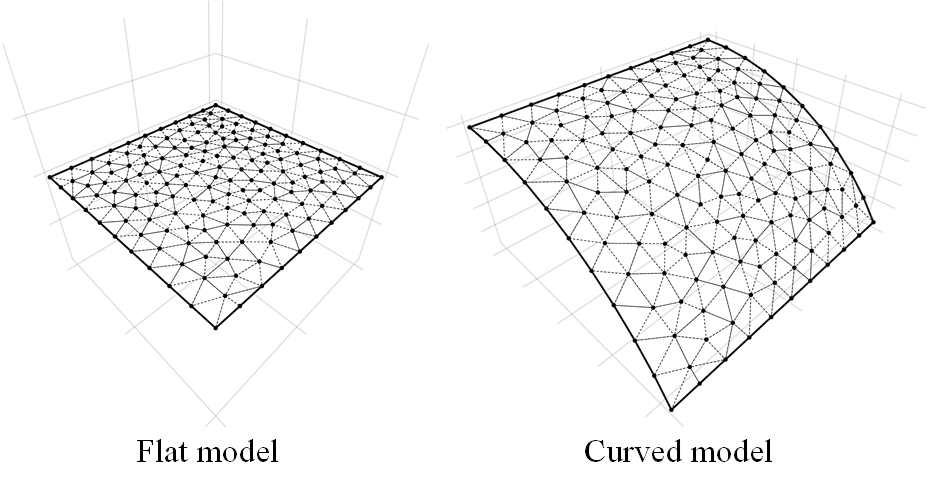
\includegraphics[width=\textwidth]{figures/ptmsh}
    \caption{Meshfree discretization for patch test}\label{ptf1}
\end{figure}

Table \ref{ptt1} lists the $L_2$- and $H_e$-Error results of patch test with flat model, where the RKGSI scheme with variational consistent essential boundary enforcement, i.e. RKGSI-Nitsche and RKGSI-HW, can pass the linear and quadratic patch test. Due to the loss of variational consistency condition, even with Nitsche's method, Gauss meshfree formulations show noticeable errors. Table \ref{ptt2} shows the results for curved model, which indicated that all the considered methods cannot pass the patch test. This is mainly because the proposed smoothed gradient of Eqs. (\ref{approxse1}) and (\ref{approxse2}) could not exactly reproduce the non-polynomial membrane and bending stress. However, the RKGSI-HW and RKGSI-Nitsche methods also provide better accuracy compared to others due to the fulfillment of first second-order variational consistency. Meanwhile, the bending moment contours of $M^{12}$ are listed in Fig. \ref{ptf2}, which further verify that the proposed method provided a satisfactory result compared to exact solution. On the other hand, the conventional Gauss meshree formulations showed errors.

\begin{table}[!ht]
\centering
\caption{Results of patch test for flat model.}\label{ptt1}
\begin{tabular}{lcccc}
\toprule
 & \multicolumn{2}{c}{Linear patch test} & \multicolumn{2}{c}{Quadratic patch test} \\ \cline{2-5}
 & $L_2$-Error & $H_e$-Error & $L_2$-Error & $H_e$-Error \\
    \midrule
    GI-Penalty & $4.45E-4$ & $1.35E-2$ & $2.01E-3$ & $1.63E-2$ \\
    GI-Nitsche & $4.51E-4$ & $1.42E-2$ & $1.22E-3$ & $1.68E-2$ \\
    RKGSI-Penalty & $3.64E-9$ & $6.77E-8$ & $4.54E-9$ & $6.57E-8$ \\
    RKGSI-Nitsche & $3.31E-12$ & $1.34E-11$ & $5.98E-12$ & $1.21E-11$ \\
    RKGSI-HR & $6.67E-13$ & $1.50E-11$ & $1.07E-12$ & $1.26E-11$ \\
    \bottomrule
\end{tabular}
\end{table}

\begin{table}[!ht]
\centering
\caption{Results of patch test for cylindrical model.}\label{ptt2}
\begin{tabular}{lcccc}
\toprule
 & \multicolumn{2}{c}{Linear patch test} & \multicolumn{2}{c}{Quadratic patch test} \\ \cline{2-5}
 & $L_2$-Error & $H_e$-Error & $L_2$-Error & $H_e$-Error \\
    \midrule
    GI-Penalty & $3.79E-4$ & $1.30E-2$ & $1.74E-3$ & $1.37E-2$ \\
    GI-Nitsche & $4.04E-4$ & $1.42E-2$ & $1.15E-3$ & $1.49E-2$ \\
    RKGSI-Penalty & $1.47E-4$ & $5.39E-3$ & $2.26E-4$ & $2.09E-3$ \\
    RKGSI-Nitsche & $2.41E-6$ & $7.37E-5$ & $2.47E-6$ & $2.89E-5$ \\
    RKGSI-HR & $4.28E-6$ & $1.30E-4$ & $9.69E-6$ & $2.41E-4$ \\
    \bottomrule
\end{tabular}
\end{table}

\begin{figure}[!ht]
\centering
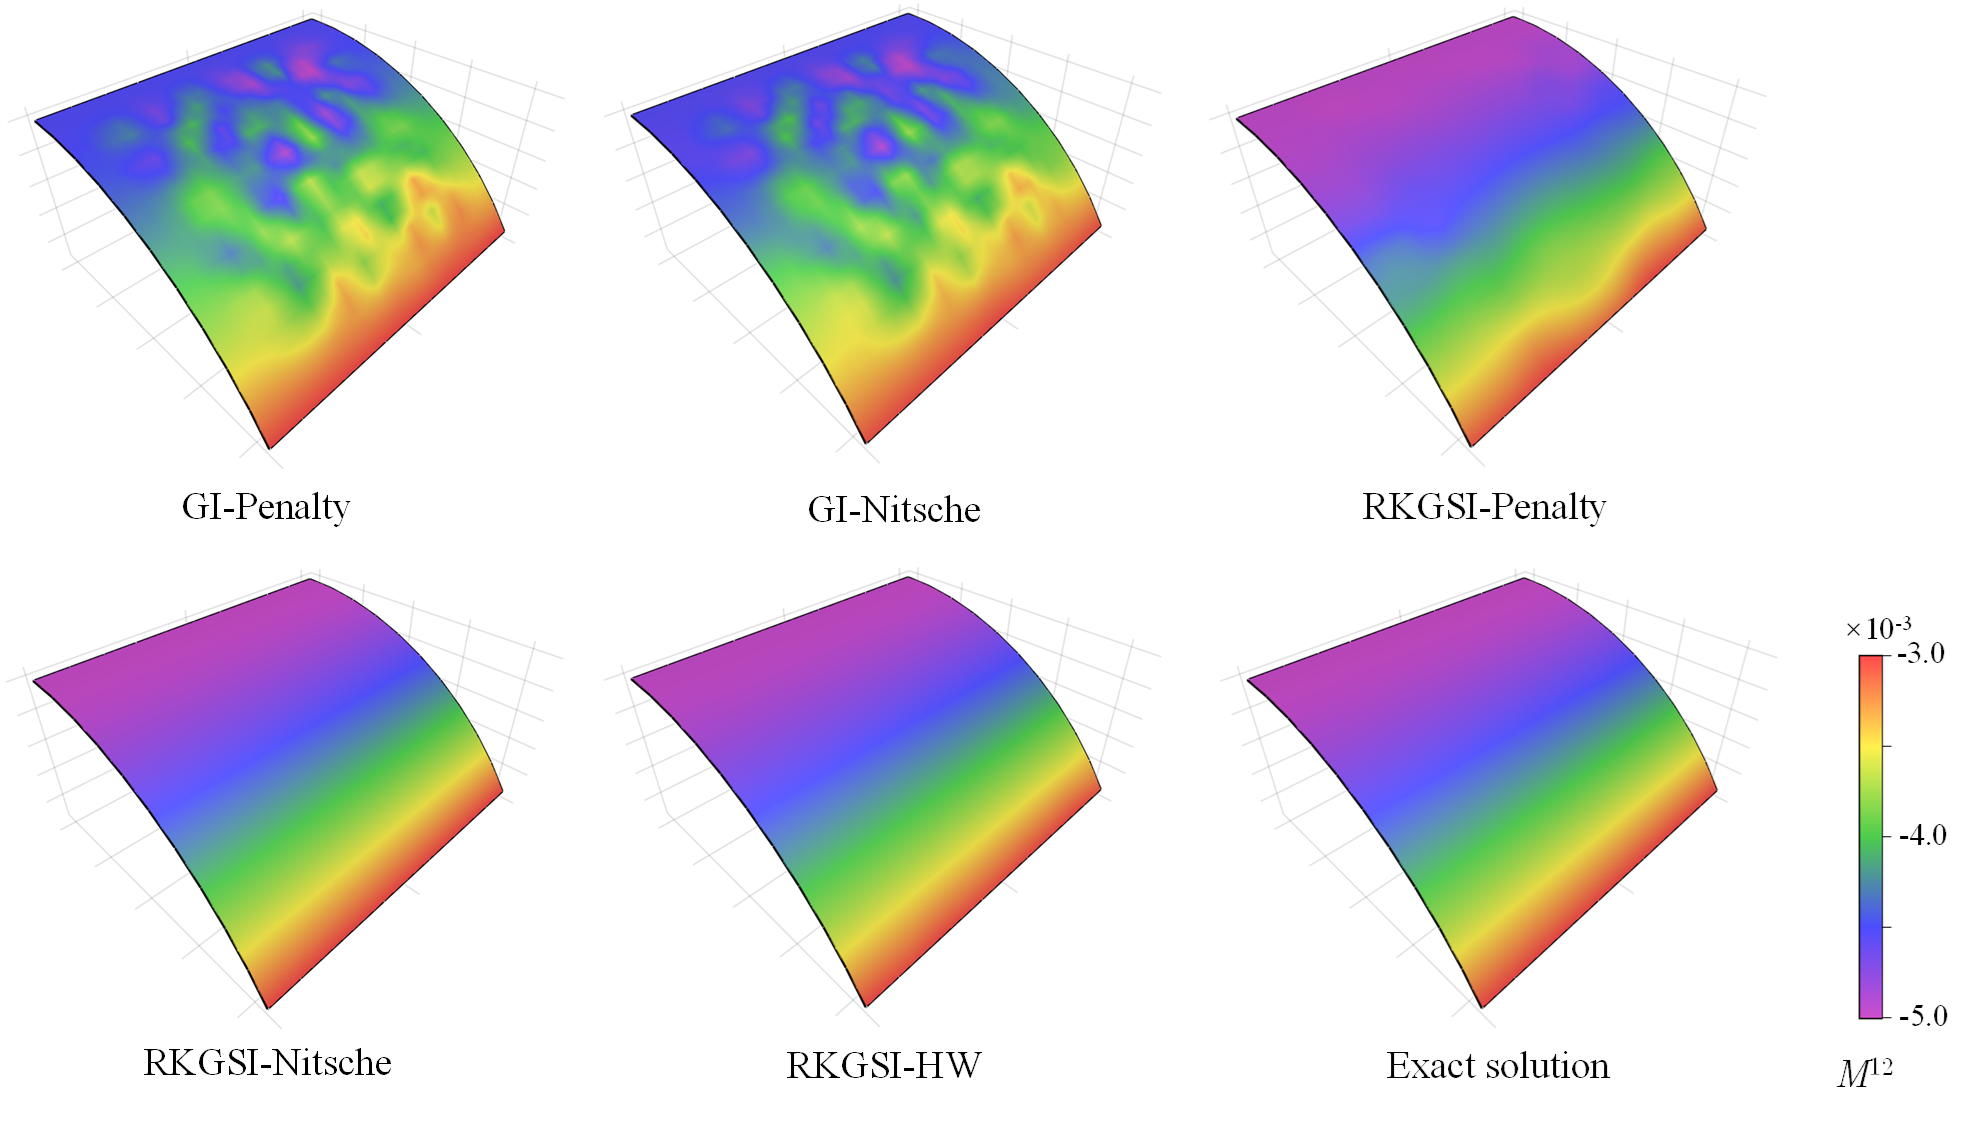
\includegraphics[width=\textwidth]{figures/ptc}
\caption{Contour plots of $M^{12}$ for curved shell patch test.}\label{ptf2}
\end{figure}

\subsection{Scordelis-Lo roof}
This example considers the classical Scordelis-Lo roof problem, as depicted in Fig. \ref{slf1}. The cylindrical roof has dimensions $R=25$, $L=50$, $h=0.25$, Young's modulus $E=4.32\times 10^8$ and Poisson's ratio $\nu=0.0$. The entire roof is subjected to an uniform body force of $b_z = -90$, with the straight edges remainning free and the the curved edges are enforced by $v_x=v_z=0$.

Due to the symmetry, only a quadrant of the model is considered for meshfree analysis, which is discretized by the $11\times 16$, $13\times 20$, $17\times 24$ and $19\times28$ meshfree nodes, as listed in Fig. \ref{slf2}. The comparison of the displacement in $z-$direction at node $A$, $v_{A3}$, is used as the investigated quantity, with the reference value 0.3024 given by \cite{macneal1985}. Firstly, Fig. \ref{slf3} presents a sensitivity study for the artificial parameters of $\alpha_v$'s, $\alpha_\theta$'s in the RKGSI meshfree formulations with Nitsche's method and penalty method. The results of Fig. \ref{slf3} revealed, Nitsche's method observed less artificial sensitivity. However, both the methods cannot trivially determine the optimal values of the artificial parameters. The optimal artificial parameters from Fig. \ref{slf3} are adopted for the convergence study in Fig. \ref{slf4}. The convergence result showed that the RKGSI get satisfactory results while the traditional Gauss methods demonstrated noticeable errors.

\begin{figure}[!ht]
\centering
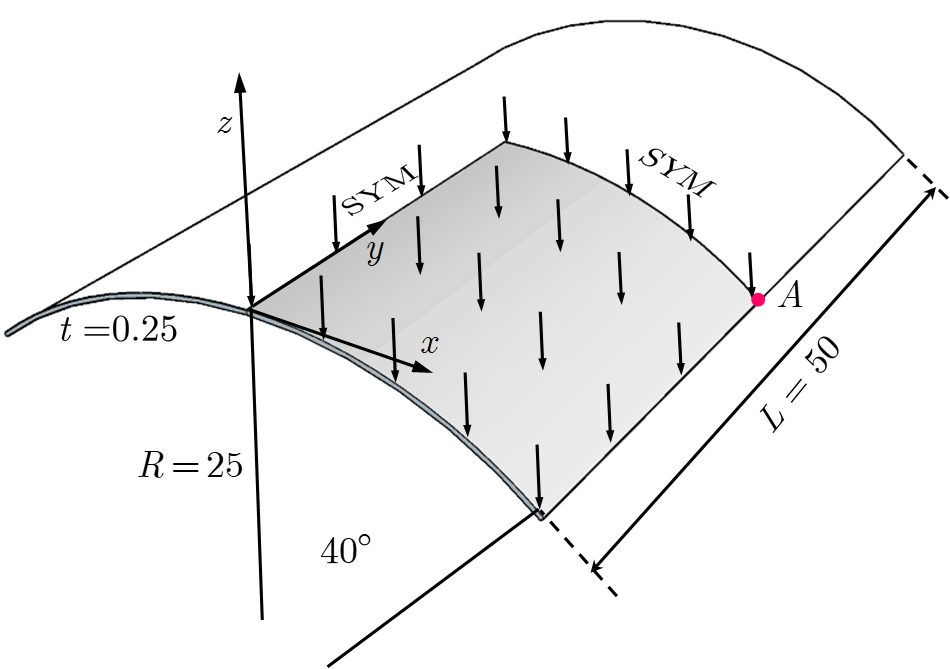
\includegraphics[width=0.7\textwidth]{figures/slm}
\caption{Description of Scordelis-Lo roof problem.}\label{slf1}
\end{figure}
\begin{figure}[!ht]
\centering
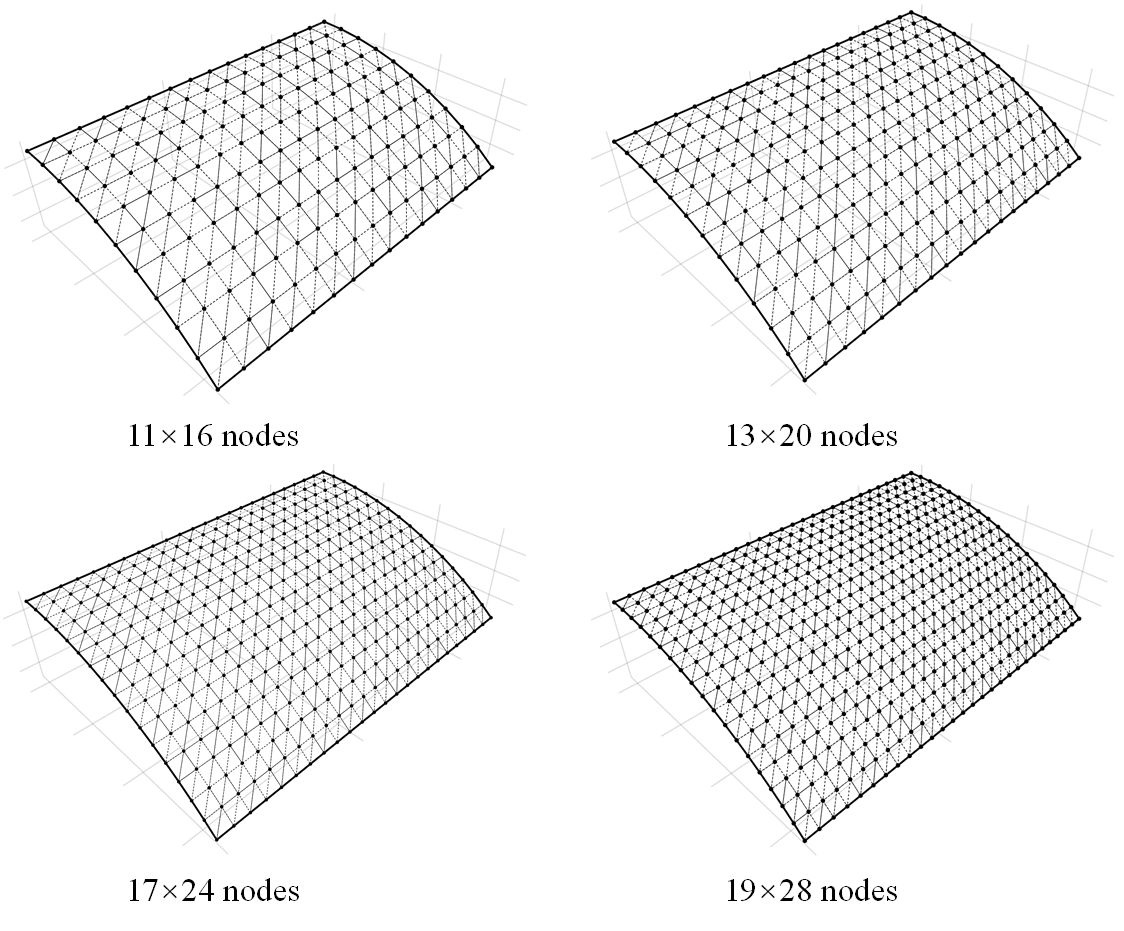
\includegraphics[width=\textwidth]{figures/slmsh}
\caption{Meshfree discretizations for Scordelis-Lo roof problem.}\label{slf2}
\end{figure}
\begin{figure}[!ht]
\centering
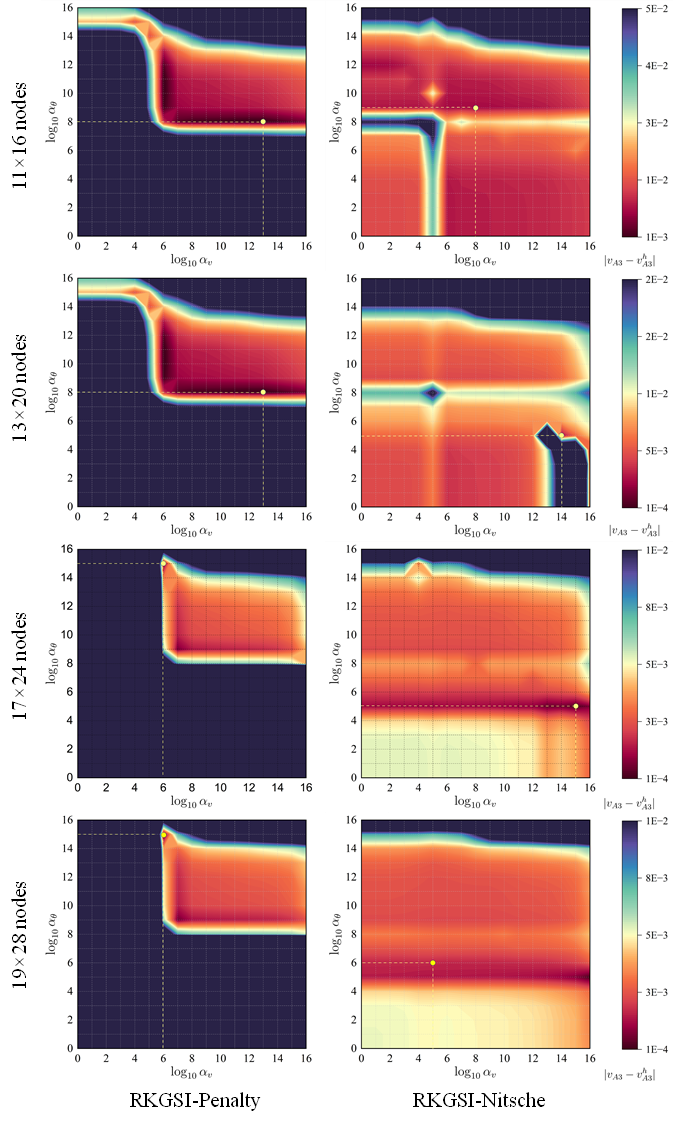
\includegraphics[width=\textwidth]{figures/sla}
\caption{Sensitivity comparison of $\alpha_v$ and $\alpha_\theta$ for Scordelis-Lo problem.}\label{slf3}
\end{figure}
\begin{figure}[!ht]
\centering
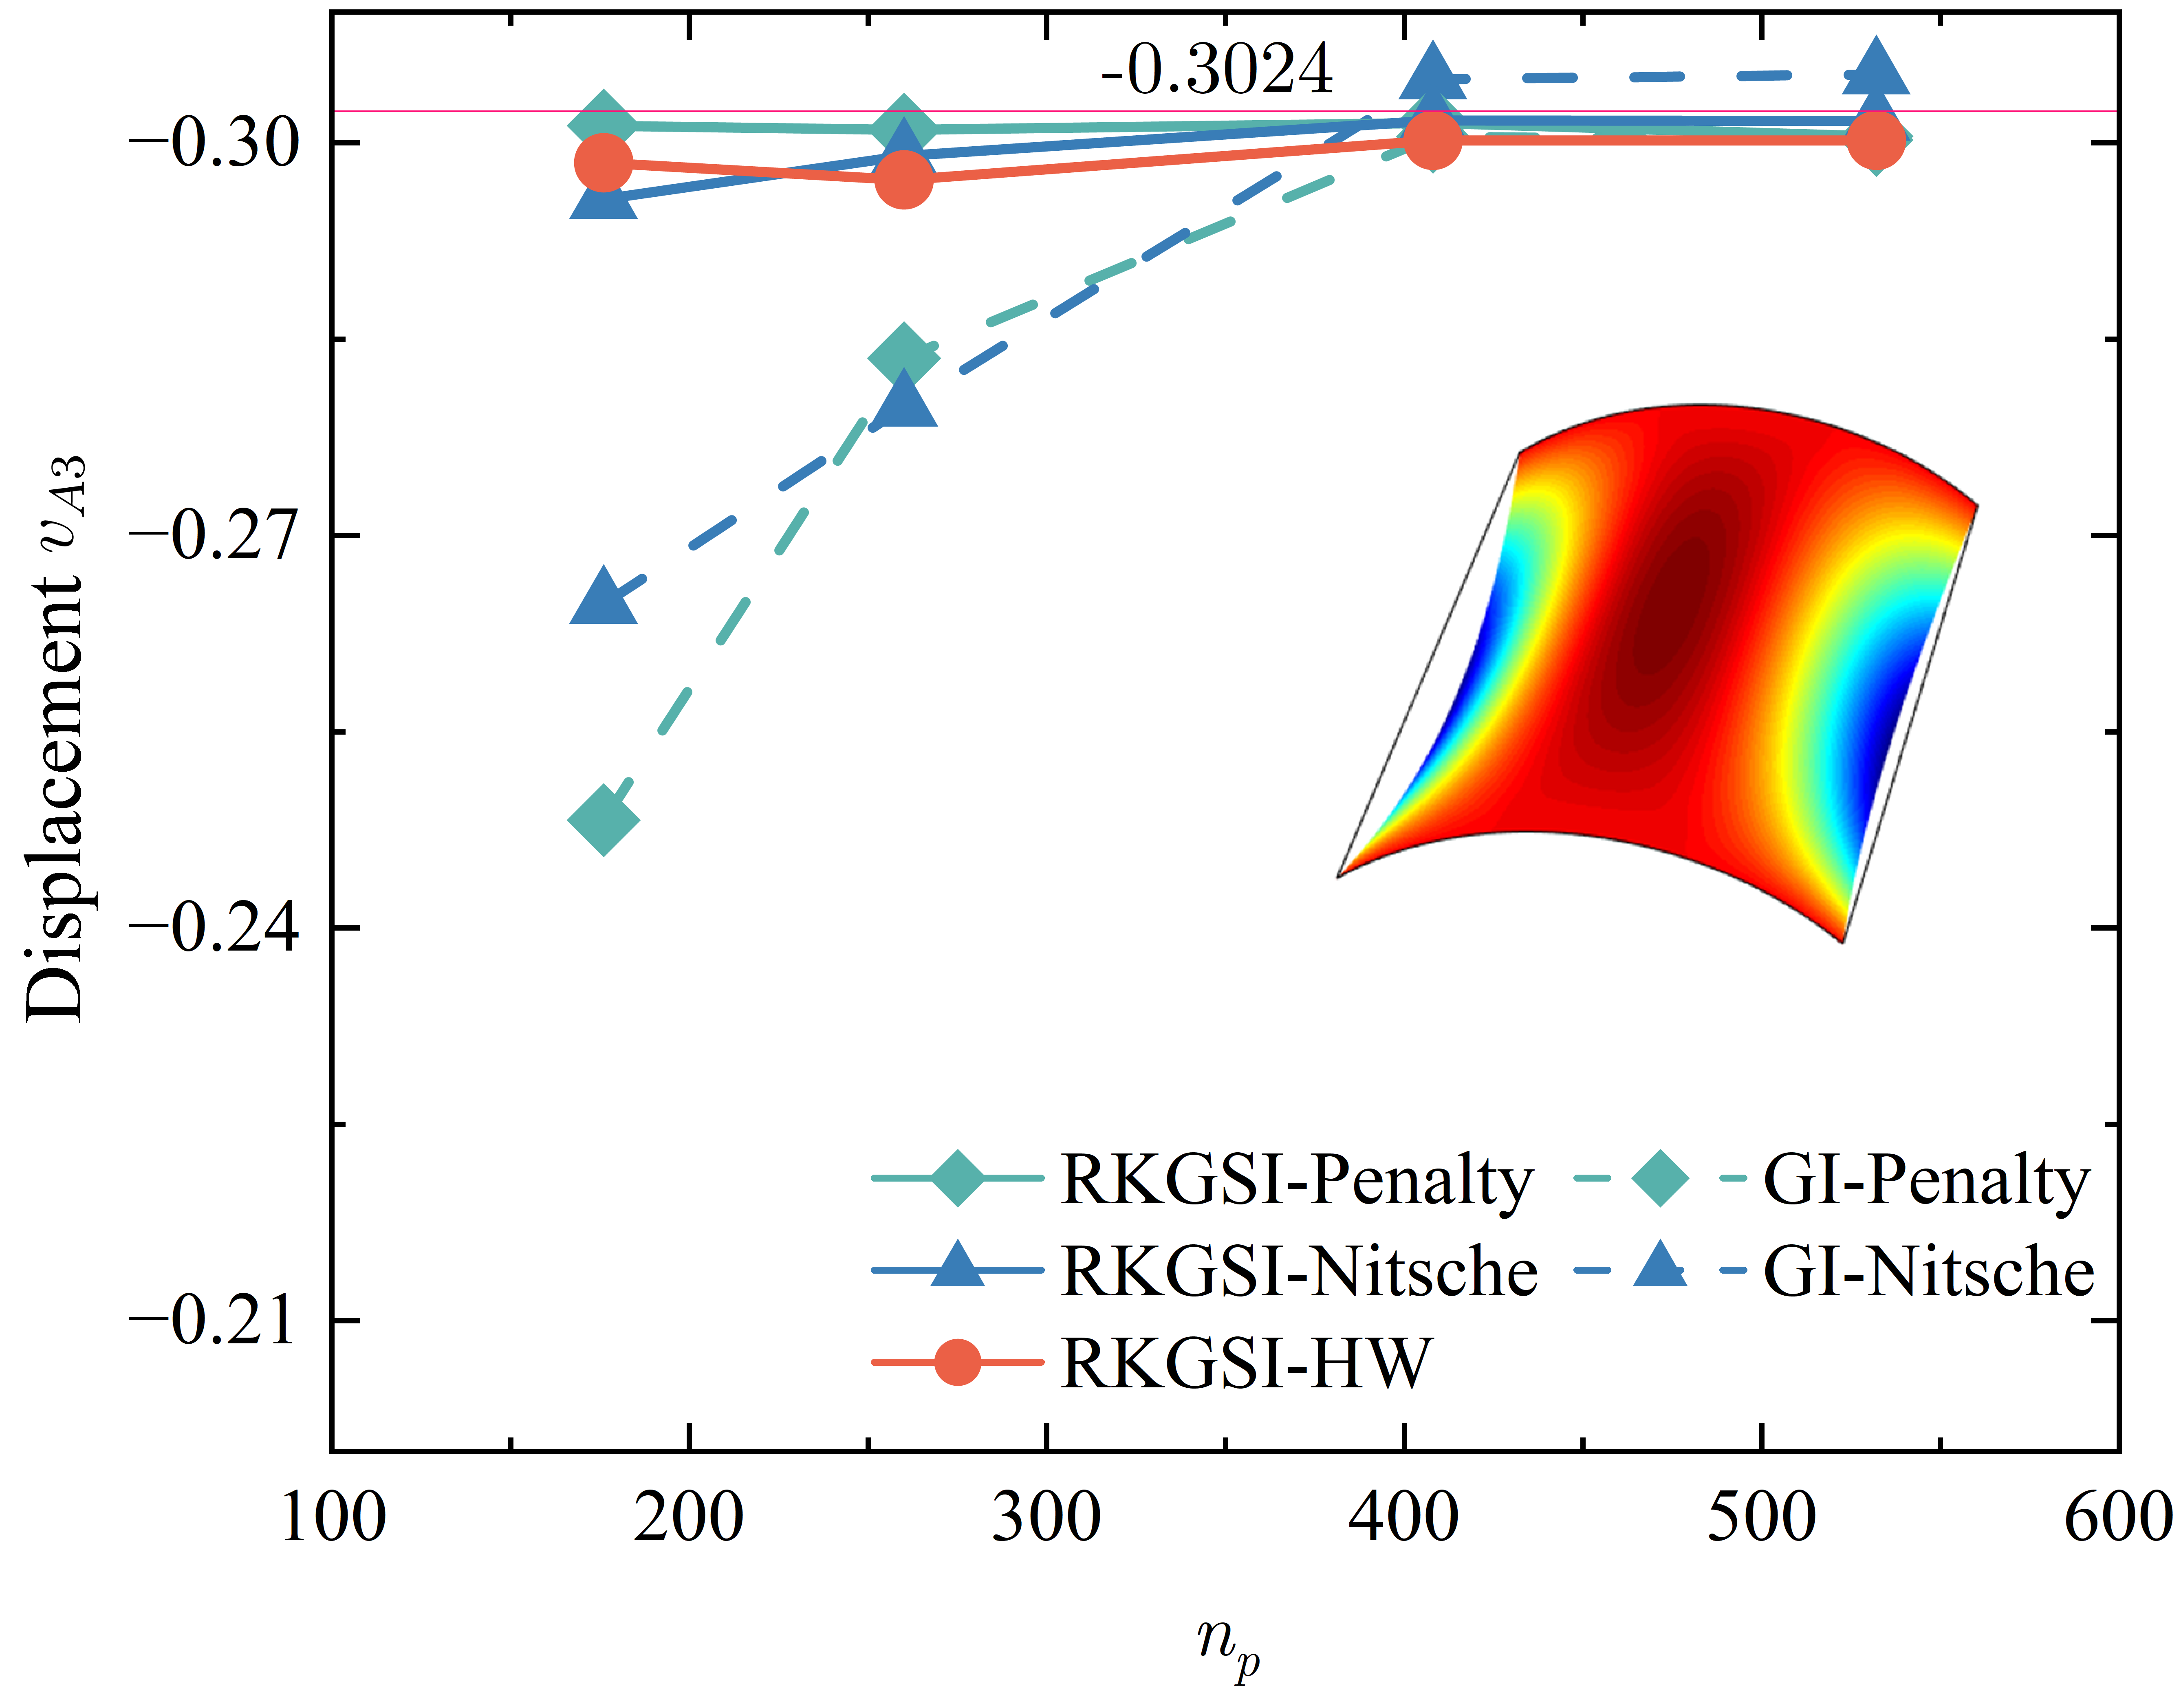
\includegraphics[width=\textwidth]{figures/sld}
\caption{Displacement convergence for Scordelis-Lo roof problem.}\label{slf4}
\end{figure}

\subsection{Pinched Hemispherical shell}
Consider the hemispherical shell shown in Fig. \ref{phf1}, which is loaded at four points $P=\pm 2$ at $90^\circ$ interval at its bottom. The hemispherical shell has an radius $R=10$, thickness $h=0.04$, Young's modulus $E=6.825\times10^7$ and Poisson's ratio $\nu = 0.3$.

Due to symmetry, only quadrant model, where the $8\times8$, $16\times16$, $24\times24$ and $32\times32$ meshfree nodes have been discretized, was considered. The quantity under investigation for convergence is the displacement at $x-$direction on point $A$, $v_{A1}$.
Fig. \ref{phf2} displays the corresponding convergence results, indicating the RKGSI scheme performed significantly better compared to the GI meshfree formulation. Meanwhile, the efficiency comparison for this problem is also shown in Fig. \ref{phf3}, in which the CPU time for assembly and calculation of shape functions are considered. Fig. \ref{phf3}(a) indicates that the RKGSI scheme observed high efficiency in assembly. This is due to the variational inconsistent Gauss meshfree formulation which require more Gaussian points to get satisfactory results. Fig. \ref{phf3}(b) lists the CPU time spent on enforcing essential boundary conditions for the penalty method, Nitsche's method and proposed HW method. The results highlighted that the proposed HW method consumed comparable CPU time in assembly compared to Nitsche's method. However, less time was spent to calculate the shape functions. Since both the HW method and penalty method were developed considering the shape functions first order derivatives. For this reason, both the methods shared an almost identical time in computing the shape functions.
\begin{figure}[!ht]
\centering
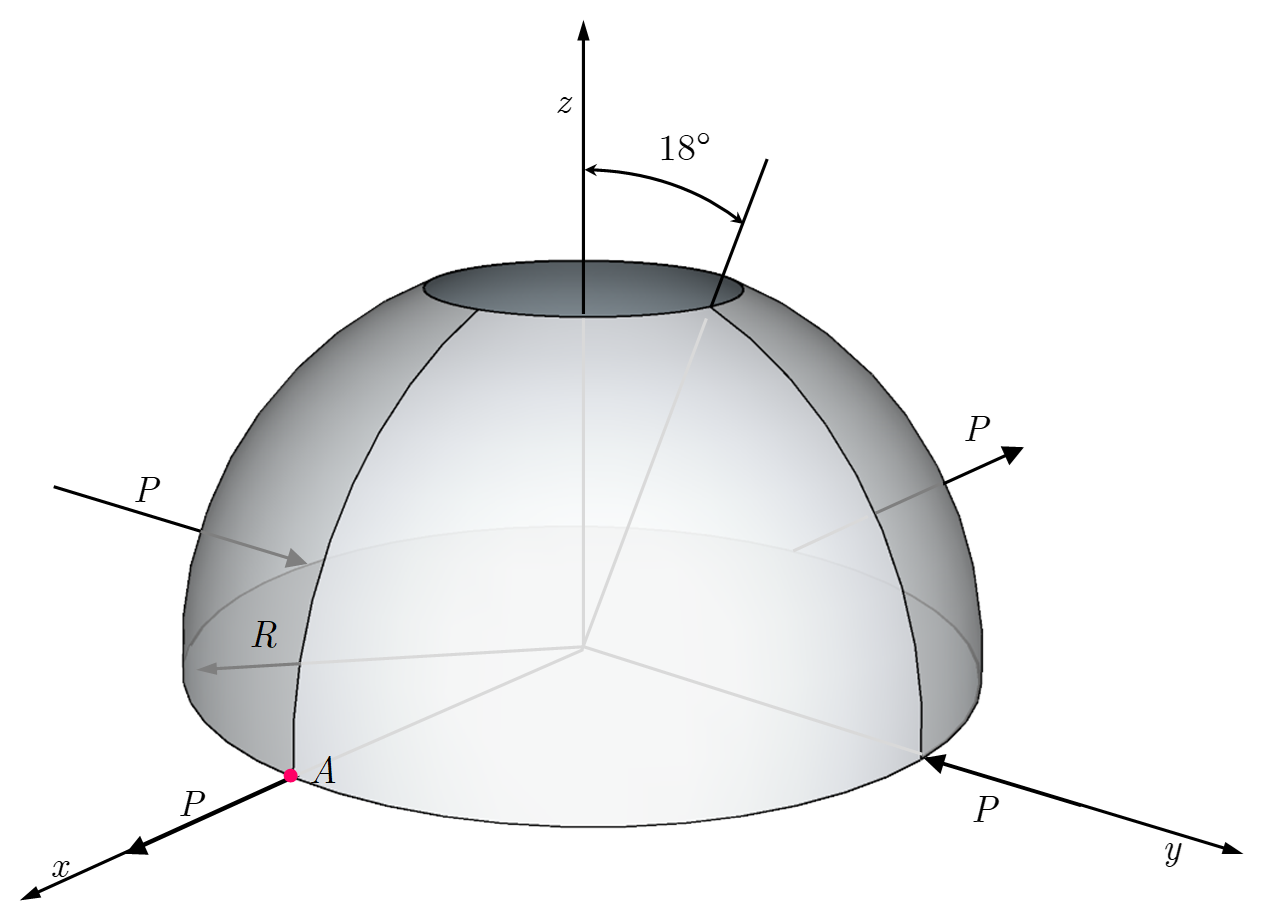
\includegraphics[width=0.8\textwidth]{figures/pfm}
\caption{Description of pinched hemispherical shell problem.}\label{phf1}
\end{figure}
\begin{figure}[!ht]
\centering
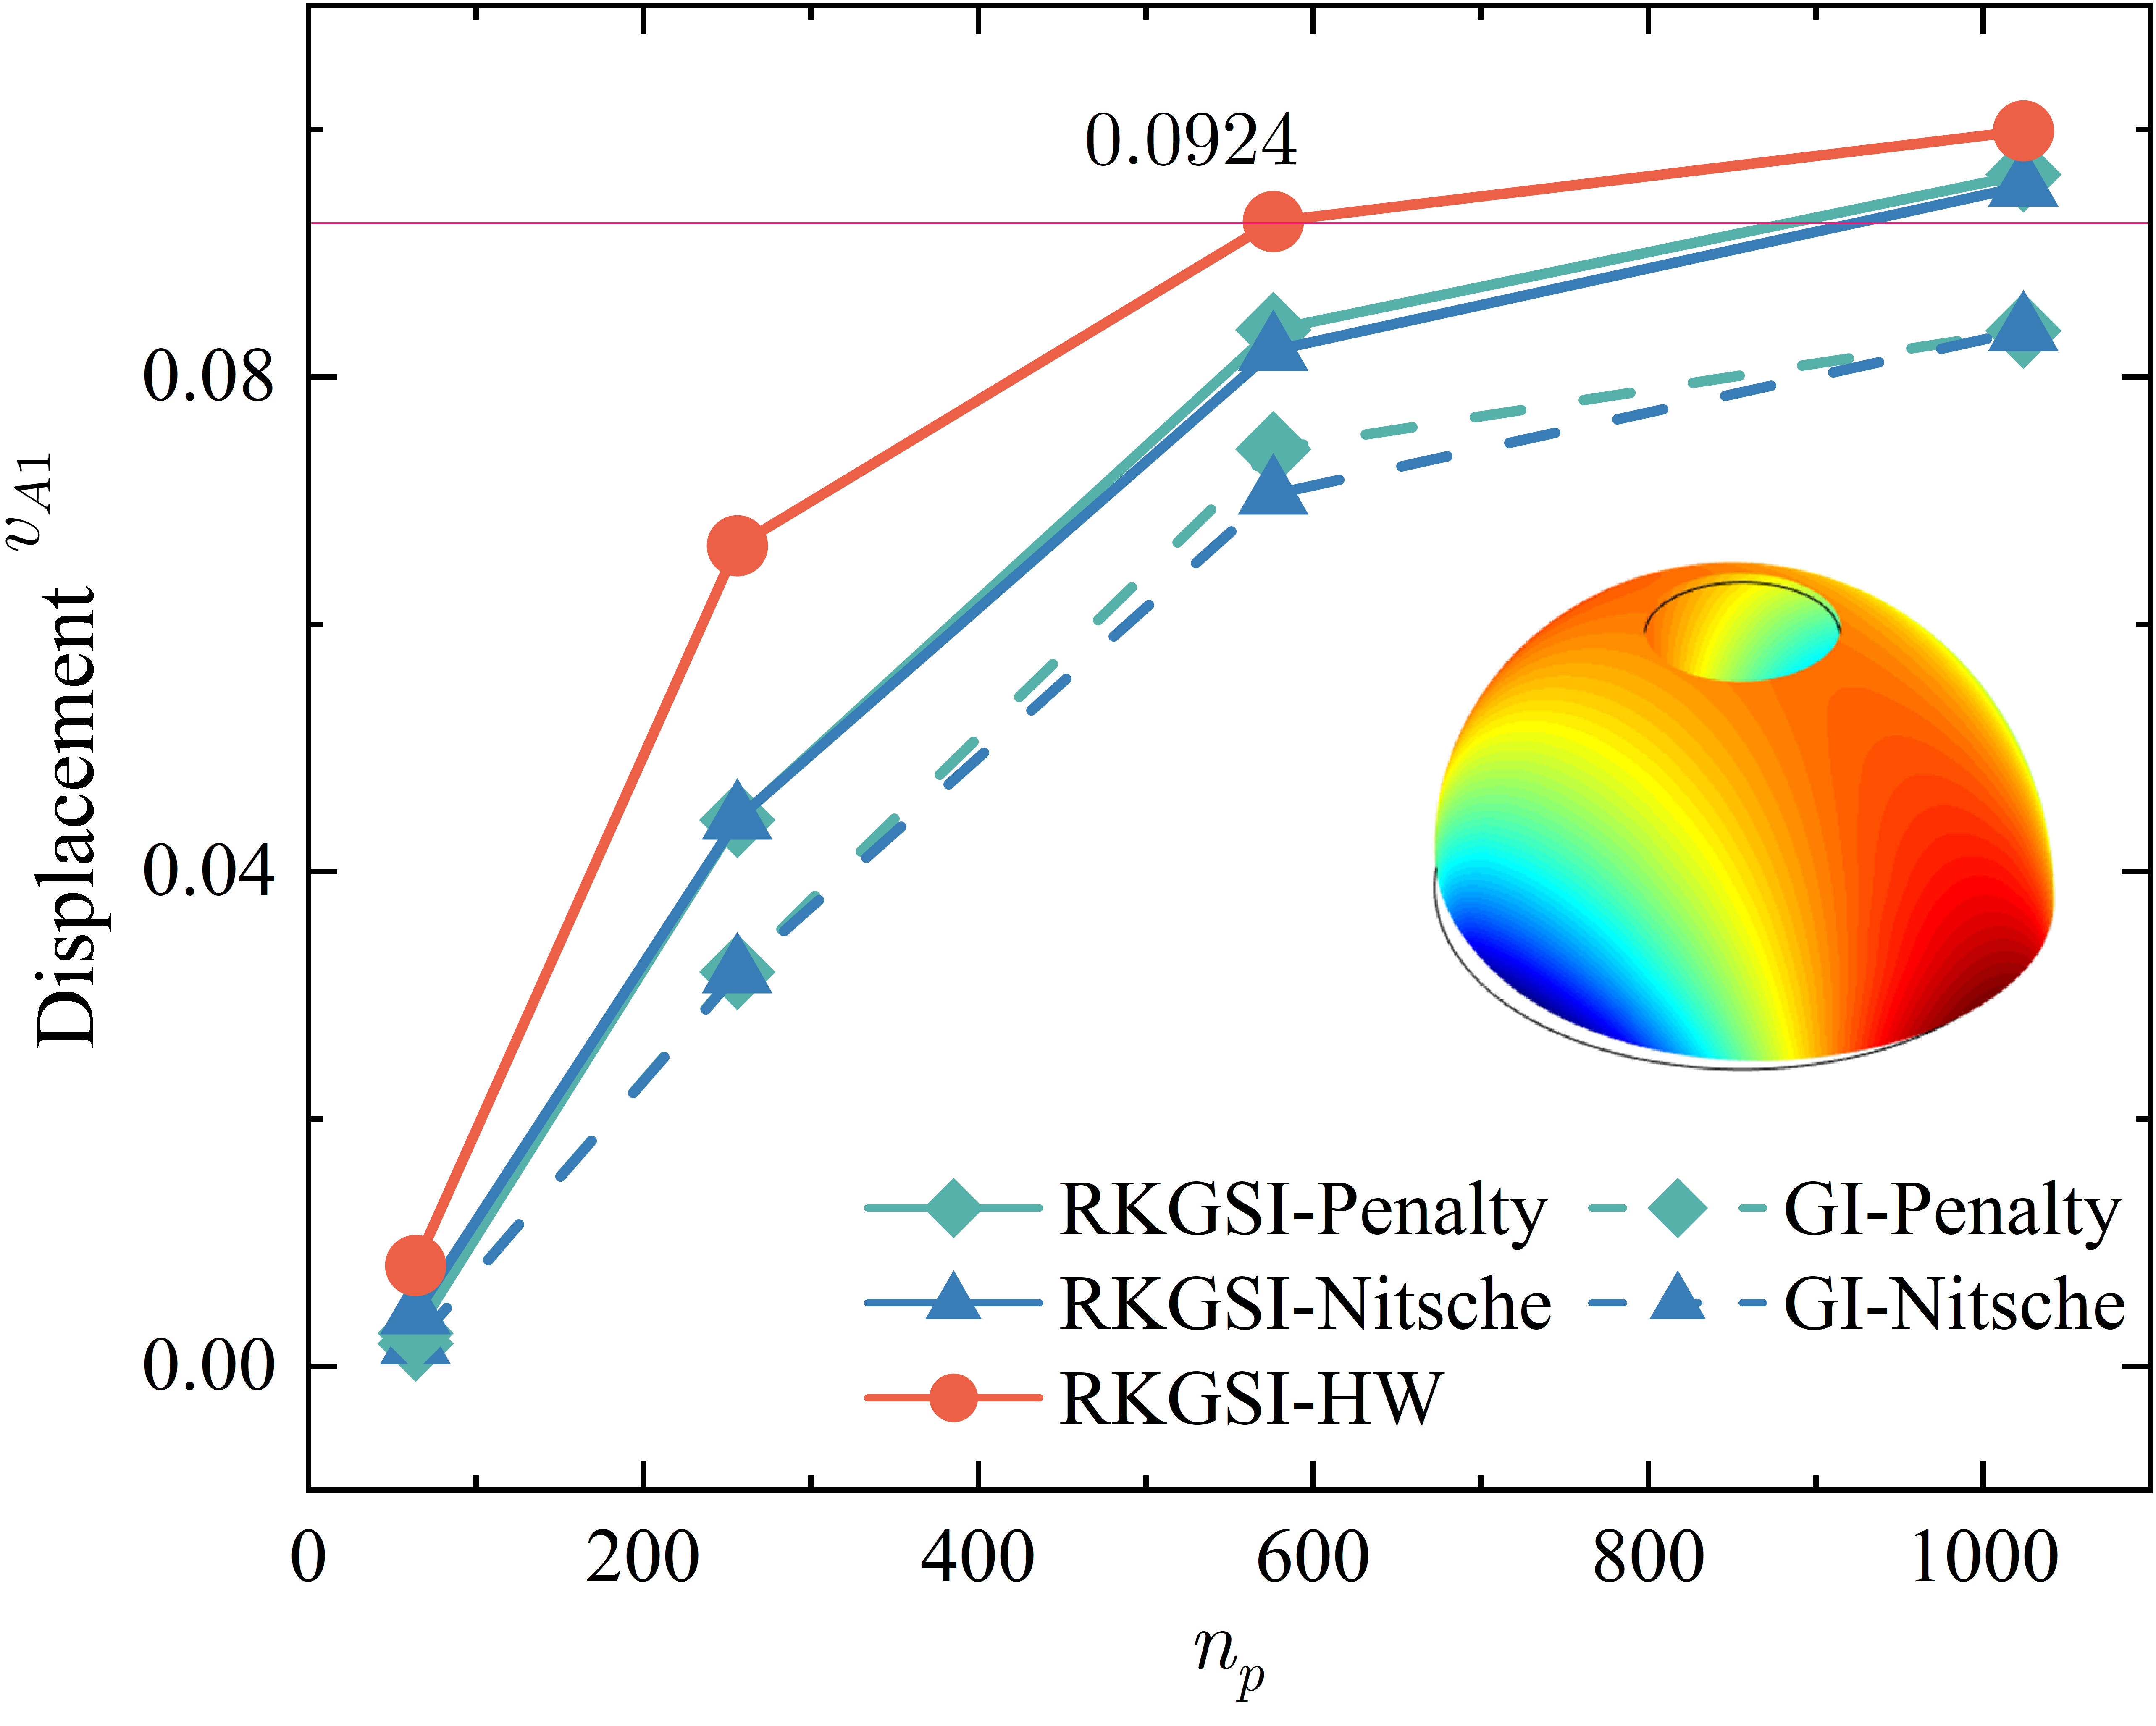
\includegraphics[width=\textwidth]{figures/pfd}
\caption{Displacement convergence for pinched hemispherical shell problem.}\label{phf2}
\end{figure}
\begin{figure}[!ht]
\centering
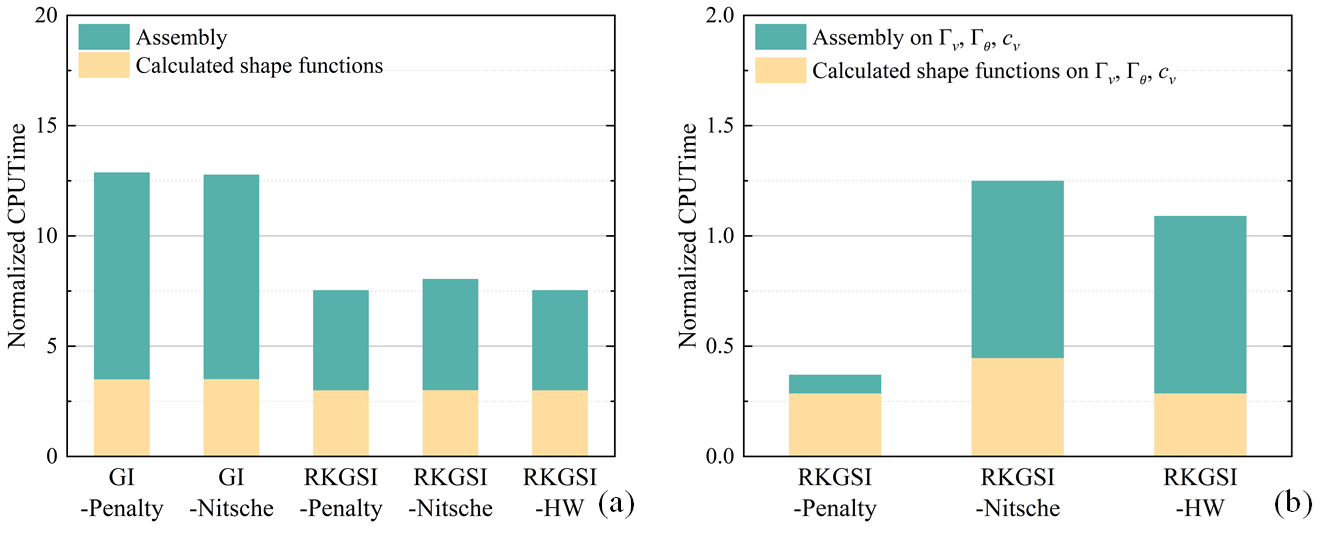
\includegraphics[width=\textwidth]{figures/efficient}
\caption{efficiency comparison for pinched hemispherical shell problem: (a) Whole domain; (b) Essential boundaries}\label{phf3}
\end{figure}



%DIFDELCMD < \section{Conclusion}\label{conclusion}
In this study, an efficient and quasi-consistent meshfree thin shell formulation was presented to naturally enforce the essential boundary conditions.  Mixed formulation with the Hu-Washizu principle weak form is adopted, where the traditional meshfree shape functions discretized the displacement, and the strains and stresses were expressed by the reproducing kernel smoothed gradients and the covariant smoothed gradients, respectively. The smoothed gradient naturally embedded the first second-order integration constraints and has a quasi variational consistency for the curved models in each integration cell. Owing to the Hu-Washizu variational principle, the essential boundary condition enforcement has a similar form with the conventional Nitsche’s method; both have consistent and stabilized terms. The costly high order derivatives in the Nitsche’s consistent term have been replaced by the smoothed gradients, which improved the computational speed due to the reproducing kernel gradient smoothing framework. Furthermore, the stabilized term naturally existed in the Hu-Washizu weak form, and the artificial parameter needed in Nitsche’s stabilized term has vanished, which can automatically maintain the coercivity for the stiffness matrix. The numerical results demonstrated that the proposed Hu-Washizu quasi-consistent meshfree thin shell formulation showed excellent accuracy, efficiency, and stability.


%DIFDELCMD < %%%
\DIFdelend \DIFaddbegin 
\begin{frontmatter}
    % \title{A Hu-Washizu variational consistent meshfree thin shell formulation naturally accommodating essential boundary conditions}
    %DIF >  \title{Quasi-consistent efficient meshfree thin shell formulation to naturally accommodate essential boundary conditions}
    \title{Quasi-consistent efficient meshfree thin shell formulation \DIFdelbegin \DIFdel{to naturally accommodate }\DIFdelend \DIFaddbegin \DIFadd{with penalty-free }\DIFaddend essential boundary \DIFdelbegin \DIFdel{conditions}\DIFdelend \DIFaddbegin \DIFadd{condition enforcement}\DIFaddend }
    \author[1]{Junchao Wu\corref{cor1}}
    \ead{jcwu@hqu.edu.cn}
    \DIFdelbegin %DIFDELCMD < \author[2]{%%%
\DIFdelend \DIFaddbegin \author[1]{\DIFaddend Yangtao Xu}
    \author[1]{Bin Xu}
    \DIFdelbegin %DIFDELCMD < \author[3]{%%%
\DIFdelend \DIFaddbegin \author[1]{\DIFaddend Syed Humayun Basha\DIFdelbegin %DIFDELCMD < \corref{cor1}%%%
\DIFdelend }
\DIFdelbegin %DIFDELCMD < \ead{syedhbasha@hqu.edu.cn}
%DIFDELCMD < %%%
\DIFdelend 

    \DIFdelbegin %DIFDELCMD < \affiliation[1]{organization={Key Laboratory for Intelligent Infrastructure and Monitoring of Fujian Province,
%DIFDELCMD <                                   College of Civil Engineering,
%DIFDELCMD <                                   Huaqiao University},
%DIFDELCMD <                     city={Xiamen},
%DIFDELCMD <                     state={Fujian},
%DIFDELCMD <                     postcode={361021},
%DIFDELCMD <                     country={China}}
%DIFDELCMD < %%%
\DIFdelend \DIFaddbegin \affiliation[1]{organization={Key Laboratory for Intelligent Infrastructure and Monitoring of Fujian Province,
                                  Key Laboratory for Structural Engineering and Disaster Prevention of Fujian Province,
                                  College of Civil Engineering,
                                  Huaqiao University},
                    city={Xiamen},
                    state={Fujian},
                    postcode={361021},
                    country={China}}
\DIFaddend 

    \DIFdelbegin %DIFDELCMD < \affiliation[2]{organization={College of Civil Engineering,
%DIFDELCMD <                                   Huaqiao University},
%DIFDELCMD <                     city={Xiamen},
%DIFDELCMD <                     state={Fujian},
%DIFDELCMD <                     postcode={361021},
%DIFDELCMD <                     country={China}}
%DIFDELCMD < 

%DIFDELCMD <     \affiliation[3]{organization={Key Laboratory for Structural Engineering and Disaster Prevention of Fujian Province,
%DIFDELCMD <                                   College of Civil Engineering,
%DIFDELCMD <                                   Huaqiao University},
%DIFDELCMD <                     city={Xiamen},
%DIFDELCMD <                     state={Fujian},
%DIFDELCMD <                     postcode={361021},
%DIFDELCMD <                     country={China}}
%DIFDELCMD < 

%DIFDELCMD <     %%%
\DIFdelend \cortext[cor1]{Corresponding author}

\begin{abstract}
This research proposed an eficient and quasi-consistent meshfree thin shell formulation with \DIFdelbegin \DIFdel{natural }\DIFdelend \DIFaddbegin \DIFadd{penalty-free }\DIFaddend enforcement of essential boundary conditions. Within the framework of the Hu-Washizu variational principle, a mixed formulation of displacements, strains and stresses is employed in this approach, where the displacements are discretized using meshfree shape functions, and the strains and stresses are expressed using smoothed gradients, covariant smoothed gradients and covariant bases. The smoothed gradients satisfy the first \DIFdelbegin \DIFdel{and second order }\DIFdelend \DIFaddbegin \DIFadd{second-order }\DIFaddend integration constraint and have \DIFdelbegin \DIFdel{quasi-consistent consistency }\DIFdelend \DIFaddbegin \DIFadd{variational consistency for polynomial strains and stresses}\DIFaddend . Owing to Hu-Washizu variational principle, the essential boundary conditions automatically arise in its weak form. As a result, the suggested technique's enforcement of essential boundary conditions resembles that of the traditional Nitsche's method. Contrary to Nitsche's method, the costly higher order derivatives of conventional meshfree shape functions were replaced by the smoothed gradients with fast computation, which improve the efficiency. Meanwhile, the proposed formulation features a naturally stabilized term without adding any artificial stabilization factors, which eliminates the \DIFdelbegin \DIFdel{stabilization parameter-dependent issue in the Nitsche's method }\DIFdelend \DIFaddbegin \DIFadd{employment of penalty method as a stabilization}\DIFaddend . The efficacy of the proposed Hu-Washizu meshfree thin shell formulation is illustrated by a set of classical standard thin shell problems.
\end{abstract}
\begin{keyword}
Meshfree \sep Thin shell \sep Hu-Washizu variational principle \sep Reproducing kernel gradient smoothing \sep Essential boundary condition
\end{keyword}
\end{frontmatter}

\section{Introduction}\label{introduction}
Thin shell structures generally adhere to the Kirchhoff hypothesis \cite{donnell1976}, that neglects the shear deformation can be described using Galerkin formulation which requires to have at least $C^1$ continuity. 
The traditional finite element methods usually \DIFdelbegin \DIFdel{only }\DIFdelend have $C^0$ continuous shape functions, and it prefers Mindlin thick shear theory, hybrid and mixed models in simulation of shell structure  \cite{hughes2000}. Meshfree methods \cite{belytschko1994,liu1995,chen2017} with high order smoothed shape functions have garnered much research attention over the past thirty years. These techniques established the shape functions based on a collection of dispersed nodes, and \DIFdelbegin \DIFdel{the }\DIFdelend high order continuity of shape functions can be easily achieved even with low-order basis functions. For thin shell analysis, \DIFdelbegin \DIFdel{this }\DIFdelend high order meshfree approximation can also \DIFaddbegin \DIFadd{furhter }\DIFaddend alleviate the membrane locking caused by the mismatched approximation order of membrane strain and bending strain \cite{krysl1996}. \DIFdelbegin \DIFdel{Furthermore}\DIFdelend \DIFaddbegin \DIFadd{Moreover}\DIFaddend , nodal-based meshfree approximations generally offer the flexibility of local refinement and can relieve the burden of mesh distortion. Owing to these benefits, numerous meshfree techniques have been developed and implemented in many scientific and engineering fields \DIFdelbegin \DIFdel{\mbox{%DIFAUXCMD
\cite{liu2009,zhang2000,millan2011,wang2023b,suchde2022,deng2023a}}\hskip0pt%DIFAUXCMD
}\DIFdelend \DIFaddbegin \DIFadd{\mbox{%DIFAUXCMD
\cite{liu2009,zhang2000,millan2011,wang2023b,suchde2022,deng2023a,wang2024}}\hskip0pt%DIFAUXCMD
}\DIFaddend . However, the high order smoothed meshfree shape functions accompany the enlarged and overlapping supports, which may potentially cause many problems for shape functions. One of the issues is the loss of the Kronecker delta property, which means that, unlike the finite element methods, the necessary boundary conditions cannot be directly enforced  \cite{fernandez-mendez2004}. Another issue is that the variational consistency or said integration constraint\DIFaddbegin \DIFadd{, which is a condition that requires the formulation to exactly reproduce the solution spanned by the basis functions, }\DIFaddend cannot be satisfied\DIFdelbegin \DIFdel{due to }\DIFdelend \DIFaddbegin \DIFadd{. This issue is mainly caused by }\DIFaddend the misalignment between the numerical integration domains and supports of shape functions. \DIFdelbegin \DIFdel{Besides}\DIFdelend \DIFaddbegin \DIFadd{Thus}\DIFaddend , the shape functions exhibit a piecewise \DIFdelbegin \DIFdel{rational }\DIFdelend nature in each integration domain. \DIFaddbegin \DIFadd{Besides, it has to be noted that the traditional integration rules like Gauss scheme cannot ensure the integration accuracy in Galerkin weak form \mbox{%DIFAUXCMD
\cite{li2016, wu2021}}\hskip0pt%DIFAUXCMD
. }\DIFaddend Therefore, variational consistency is vital to the solution accuracy in \DIFdelbegin \DIFdel{Galerkin formulations \mbox{%DIFAUXCMD
\cite{li2016, wu2021}}\hskip0pt%DIFAUXCMD
}\DIFdelend \DIFaddbegin \DIFadd{the Galerkin meshfree formulations}\DIFaddend .

Various ways have been presented to enforce the necessary boundary for Galerkin meshfree methods directly, including the boundary singular kernel method \cite{chen2000a}, mixed transformation method  \cite{chen2000a}, and interpolation element-free method \cite{liu2019a} for recovering shape functions’ Kronecker property. However, these methods \DIFdelbegin \DIFdel{are }\DIFdelend \DIFaddbegin \DIFadd{were }\DIFaddend not based on \DIFdelbegin \DIFdel{a }\DIFdelend variational setting and cannot guarantee variational consistency. In the absence of a meshfree node, accuracy enforcement might be \DIFdelbegin \DIFdel{poorer}\DIFdelend \DIFaddbegin \DIFadd{poor}\DIFaddend . In contrast, enforcing the essential boundary conditions using a variational approach is preferred for Galerkin meshfree methods. The variational consistent Lagrange multiplier approach was initially used to the Galerkin meshfree method by Belytschko et al. \cite{belytschko1994}. In this method, the extra degrees of freedom are used to determine the discretion of Lagrange multiplier. \DIFdelbegin \DIFdel{Furthermore, }\DIFdelend Ivannikov et al. \cite{ivannikov2014a} \DIFdelbegin \DIFdel{have }\DIFdelend extended this approach to geometrically nonlinear thin shells. Lu et al. \cite{lu1994} suggested the modified variational essential boundary enforcement approach and expressed the Lagrange multiplier by equivalent tractions to eliminate the excess degrees of freedom. However, the coercivity of this approach is not always ensured and potentially reduces the accuracy. Zhu and Atluri \cite{zhu1998} pioneered the penalty method for meshfree method, making it a straightforward approach to enforce essential boundary conditions via Galerkin weak form. However, the penalty method lacks variational consistency and requires experimental artificial parameters whose optimal value is hard to determine. Fernández-Méndez and Huerta \cite{fernandez-mendez2004} imposed necessary boundary conditions using Nitsche's approach in the meshfree formulation. This approach can be seen as a hybrid combination of the modified variational method and the penalty method because the modified variational method generates variational consistency through the use of a consistent term, and the penalty method is used as a stabilized term to recover the coercivity. Skatulla and Sansour \cite{skatulla2008} extended Nitsche’s thin shell analysis method and proposed an iteration algorithm to determine artificial parameters at each integration point.

In order to address the issue of numerical integration, a series of consistent integration schemes have been developed for Galerkin meshfree methods. Among these include stabilized conforming nodal integration \cite{chen2001} , variational consistent integration \cite{chen2013a}, quadratic consistent integration \cite{duan2012a}, reproducing kernel gradient smoothing integration \cite{wang2019a}, and consistent projection integration  \cite{wang2023}. The assumed strain approach establishes the most consistent integration scheme, while the smoothed gradient replaces the costly higher order derivatives of traditional meshfree shape functions and shows a high efficiency. Moreover, to achieve global variational consistency, a consistent essential boundary condition enforcement \DIFdelbegin \DIFdel{should cooperate }\DIFdelend \DIFaddbegin \DIFadd{must be combined }\DIFaddend with the consistent integration scheme. The \DIFaddbegin \DIFadd{combination of }\DIFaddend consistent integration scheme and Nitsche’s method for treating essential boundary conditions \DIFdelbegin \DIFdel{show a good performance since they }\DIFdelend \DIFaddbegin \DIFadd{may demonstrate better performance since both the methods }\DIFaddend can satisfy the coercivity without requiring additional degrees of freedom. Nevertheless, Nitsche's approach still retains the artificial parameters in \DIFaddbegin \DIFadd{the }\DIFaddend stabilized terms, and it is essential to remain \DIFdelbegin \DIFdel{conscious }\DIFdelend \DIFaddbegin \DIFadd{cautious }\DIFaddend of the costly higher order derivatives, particularly for thin plate and thin shell problems. Recently, Wu et al. \cite{wu2022a,wu2023}  proposed an efficient and stabilized essential boundary condition enforcement method based upon the Hellinger-Reissner variational principle, where a mixed formulation in Hellinger-Reissner weak form recasts the reproducing kernel gradient smoothing integration. The terms \DIFaddbegin \DIFadd{required }\DIFaddend for enforcing essential boundary conditions are identical to the Nitsche’s method, and both have consistent and stabilized terms. \DIFdelbegin \DIFdel{Nevertheless}\DIFdelend \DIFaddbegin \DIFadd{However}\DIFaddend , the stabilized term of this method naturally exists in the Hellinger-Reissner weak form and no longer needs the artificial parameters, even for essential boundary enforcement\DIFdelbegin \DIFdel{; instead }\DIFdelend \DIFaddbegin \DIFadd{. Instead }\DIFaddend all of the higher order derivatives are represented by \DIFaddbegin \DIFadd{the }\DIFaddend smoothed gradients and their derivatives.

In this study, an efficient and stabilized variational consistent meshfree method that naturally enforces the essential boundary conditions is developed for thin shell \DIFdelbegin \DIFdel{structure}\DIFdelend \DIFaddbegin \DIFadd{structures}\DIFaddend . Following the concept of the Hellinger-Reissner principle base consistent meshfree method, the Hu-Washizu variational principle of complementary energy with variables of displacement, strains, and stresses \DIFdelbegin \DIFdel{is }\DIFdelend \DIFaddbegin \DIFadd{were }\DIFaddend employed. The displacement is approximated by conventional meshfree shape functions, and the strains and stresses \DIFdelbegin \DIFdel{are }\DIFdelend \DIFaddbegin \DIFadd{were }\DIFaddend expressed by smoothed gradients with covariant bases. It is important to note that although the first second-order integration requirements \DIFdelbegin \DIFdel{are }\DIFdelend \DIFaddbegin \DIFadd{were }\DIFaddend naturally embedded in the smoothed gradients, their fulfillment \DIFdelbegin \DIFdel{can only result }\DIFdelend \DIFaddbegin \DIFadd{resulted }\DIFaddend in a quasi-satisfaction of variational consistency\DIFaddbegin \DIFadd{. This is mainly }\DIFaddend because of the non-polynomial nature of the stresses. Hu-Washizu's weak form \DIFdelbegin \DIFdel{is }\DIFdelend \DIFaddbegin \DIFadd{was }\DIFaddend used to evaluate all the essential boundary conditions regarding displacements and rotations. This type of formulation is similar to the Nitsche's method but does not require any artificial parameters. Compared with Nitsche’s method, conventional reproducing smoothed gradients and its direct derivatives replace the costly higher order derivatives. By utilizing the advantages of a replicating kernel gradient smoothing framework, the smoothed gradients showed better performance compared to conventional derivatives of shape functions, hence increasing the meshfree formulation's computational efficiency.

The remainder of this research \DIFdelbegin \DIFdel{paper }\DIFdelend \DIFaddbegin \DIFadd{article }\DIFaddend is structured as follows: The kinematics of the thin shell structure and the weak form of the associated Hu-Washizu principle are briefly described in Section 2. \DIFdelbegin \DIFdel{Subsequently, the }\DIFdelend \DIFaddbegin \DIFadd{The }\DIFaddend mixed formulation regarding the displacements, strains and stresses in accordance with Hu-Washizu weak form are presented in Section 3. The discrete equilibrium equations are derived in Section 4 using the naturally occurring accommodation of essential\DIFdelbegin \DIFdel{, and }\DIFdelend \DIFaddbegin \DIFadd{. Subsequently, }\DIFaddend they are compared to the equations obtained using Nitsche's method. The numerical results in Section 5 validate the efficacy of the proposed Hu-Washizu meshfree thin shell formulation. Lastly, the concluding remarks are presented in Section 6.


\section{Hu-Washizu's formulation of complementary energy for thin shell}\label{Kinematics}
\subsection{Kinematics for thin shell}
Consider the configuration of a shell $\bar \Omega$, as shown in Fig. \ref{fig1}, which can be easily described by a parametric curvilinear coordinate system $\boldsymbol \xi = \{\xi^i\}_{i=1,2,3}$. The mid-surface of the shell denoted by $\Omega$ is specified by the in-plane coordinates $\boldsymbol \xi = \{\xi^\alpha\}_{\alpha=1,2}$, as the thickness direction of shell is by $\xi^3$, $-\frac{h}{2} \le \xi^3 \le \frac{h}{2}$, $h$ is the thickness of shell. In this work, Latin indices take the values from 1 to 3, and Greek indices are evaluated by 1 or 2. For the Kirchhoff hypothesis \cite{krysl1996}, the position $\boldsymbol x\in \bar \Omega$ is defined by linear functions with respect to $\xi^3$ :
\begin{equation}\label{x}
\boldsymbol x(\xi^1, \xi^2, \xi^3) = \boldsymbol r(\xi^1,\xi^2) + \xi^3 \boldsymbol a_3(\xi^1,\xi^2)
\end{equation}
\begin{figure}[!ht]
\centering
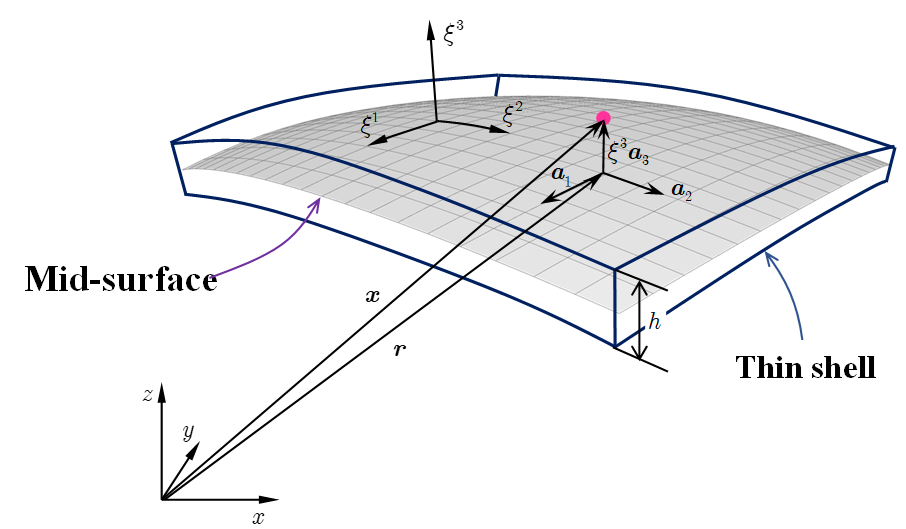
\includegraphics[width=0.7\textwidth]{figures/1}
\caption{Kinematics for thin shell.}\label{fig1}
\end{figure}
in which $\boldsymbol r$ means the position on the mid-surface of shell, and $\boldsymbol a_3$ is corresponding normal direction. For the mid-surface of shell, the in-plane covariant base vector with respect to $\xi^\alpha$ can be derived by a trivial partial differentiation to $\boldsymbol r$:
\begin{equation}
\boldsymbol a_\alpha = \frac{\partial \boldsymbol r}{\partial \xi^\alpha} = \boldsymbol r_{,\alpha}, \alpha  = 1,2
\end{equation}
to provide for a clear expression, the subscript comma denotes the partial differentiation operation with respect to in-plane coordinates $\xi^\alpha$, and the normal vector $\boldsymbol a_3$ can be obtained by the normalized cross product of $\boldsymbol a_{\alpha}$'s as follows:
\begin{equation}
\boldsymbol a_3 = \frac{\boldsymbol a_1 \times \boldsymbol a_2}{\Vert \boldsymbol a_1 \times \boldsymbol a_2 \Vert}
\end{equation}
where $\Vert \bullet \Vert$ is the Euclidean norm operator.

With the assumption of infinitesimal deformation, the strain components with respect to the global contravariant base can be stated as:
\begin{equation}\label{epsilon}
\epsilon_{ij} = \frac{1}{2}(\boldsymbol x_{,i} \cdot \boldsymbol u_{,j} + \boldsymbol u_{,i} \cdot \boldsymbol x_{,j})
\end{equation}
where $\boldsymbol u$ represents the displacement for the shell deformation. To satisfy the Kirchhoff hypothesis, the displacement is assumed to be of the following form:
\begin{equation}\label{u}
\boldsymbol u(\xi^1,\xi^2,\xi^3) = \boldsymbol v(\xi^1,\xi^2) + \boldsymbol \theta(\xi^1,\xi^2) \xi^3
\end{equation}
in which the quadratic and higher order terms are neglected. $\boldsymbol v$, $\boldsymbol \theta$ resperesent the displacement and rotation in mid-surface, respectively.

Subsequently, plugging Eqs. (\ref{x}) and (\ref{u}) into Eq. (\ref{epsilon}) and neglecting the quadratic terms, the strain components can be rephrased as follows:
\begin{subequations}
\begin{align}
\begin{split}
\epsilon_{\alpha\beta} &= \frac{1}{2}(\boldsymbol a_\alpha \cdot \boldsymbol v_{,\beta} + \boldsymbol v_{,\alpha}\cdot \boldsymbol a_\beta) \\ 
&+ \frac{1}{2}(\boldsymbol a_{3,\alpha} \cdot \boldsymbol v_{,\beta} + \boldsymbol v_{,\alpha}\cdot \boldsymbol a_{3,\beta} + \boldsymbol a_\alpha \cdot \boldsymbol \theta_{,\beta} + \boldsymbol \theta_{,\alpha}\cdot \boldsymbol a_\beta)\xi^3 \\
&= \varepsilon_{\alpha\beta} + \kappa_{\alpha\beta}\xi^3
\end{split} \\
\epsilon_{\alpha 3} &= \frac{1}{2}(\boldsymbol a_\alpha \cdot \boldsymbol \theta + \boldsymbol v_{,\alpha}\cdot \boldsymbol a_3) + \frac{1}{2} (\boldsymbol a_3 \cdot \boldsymbol \theta)_{,\alpha}\xi^3 \\ 
\epsilon_{33} &= \boldsymbol a_3 \cdot \boldsymbol \theta
\end{align}
\end{subequations}
where $\varepsilon_{\alpha\beta}$, $\kappa_{\alpha\beta}$ represent membrane and bending strains, respectively, and are given as follows:
\begin{equation}
\varepsilon_{\alpha\beta} = \frac{1}{2}(\boldsymbol a_\alpha \cdot \boldsymbol v_{,\beta} + \boldsymbol v_{,\alpha}\cdot \boldsymbol a_\beta) 
\end{equation}
\begin{equation}\label{kappa1}
\kappa_{\alpha\beta} = \frac{1}{2}(\boldsymbol a_{3,\alpha} \cdot \boldsymbol v_{,\beta} + \boldsymbol v_{,\alpha}\cdot \boldsymbol a_{3,\beta} + \boldsymbol a_\alpha \cdot \boldsymbol \theta_{,\beta} + \boldsymbol \theta_{,\alpha}\cdot \boldsymbol a_\beta)
\end{equation}

In accordance with the Kirchhoff hypothesis, the thickness of shell will not change, and the deformation related with direction of $\xi^3$ will vanish, i.e. $\epsilon_{3i}=0$. Thus, the rotation $\boldsymbol \theta$ can be rewritten as:
\begin{equation}\label{a3}
\epsilon_{3i} = 0 \Rightarrow
\left \{
\begin{split}
&\boldsymbol \theta \cdot \boldsymbol a_\alpha \DIFdelbegin \DIFdel{+ }\DIFdelend \DIFaddbegin \DIFadd{=- }\DIFaddend \boldsymbol v_{,\alpha} \cdot \boldsymbol a_3 \DIFdelbegin \DIFdel{= 0 }\DIFdelend \\
&\boldsymbol \theta \cdot \boldsymbol a_3 = 0
\end{split}
\right .
\Rightarrow \boldsymbol \theta = - \boldsymbol v_{,\alpha} \cdot \boldsymbol a_3 \boldsymbol a^\alpha
\end{equation}
where $\boldsymbol a^\alpha$'s is the in-plane contravariant base vector, $\boldsymbol a^\alpha \cdot \boldsymbol a_\beta = \delta^\alpha_\beta$, $\delta$ is the Kronecker delta function. \DIFdelbegin \DIFdel{Substituting Eq. }\DIFdelend \DIFaddbegin \DIFadd{The detailed derivation of Eq. \ref{a3} can be found in \mbox{%DIFAUXCMD
\cite{benzaken2021}}\hskip0pt%DIFAUXCMD
.
}

\DIFadd{Furthermore, on substituting Eq. }\DIFaddend (\ref{a3}) into Eq. (\ref{kappa1}) leads to:
\begin{equation}
\kappa_{\alpha\beta} = (\Gamma^\gamma_{\alpha\beta} \boldsymbol v_{,\gamma} - \boldsymbol v_{,\alpha\beta}) \cdot \boldsymbol a_3 = - \boldsymbol v_{,\alpha}\vert_\beta \cdot \boldsymbol a_3
\end{equation}
in which $\Gamma^\gamma_{\alpha\beta} = \boldsymbol a_{\alpha,\beta} \cdot \boldsymbol a^\gamma$ is namely the Christoffel symbol of the second kind, and \DIFdelbegin \DIFdel{$\boldsymbol v_{,\alpha}\vert\beta$ }\DIFdelend \DIFaddbegin \DIFadd{$\boldsymbol v_{,\alpha}\vert_\beta$ }\DIFaddend is the in-plane covariant derivative of $\boldsymbol v_{,\alpha}$, i.e. $\boldsymbol v_{,\alpha}\vert_\beta = \Gamma^\gamma_{\alpha\beta}\boldsymbol v_{,\gamma} - \boldsymbol v_{,\alpha\beta}$.

\subsection{Galerkin weak form for Hu-Washizu principle of complementary energy}
In this study, the Hu-Washizu variational principle of complementary energy \cite{dah-wei1985} was adopted for the development of the proposed analytical approach, the corresponding complementary functional, denoted by $\Pi_C$, is listed as follows:
\begin{equation} \label{functionalc}
\begin{split}
&\Pi_C(\varepsilon_{\alpha\beta},\kappa_{\alpha\beta},N^{\alpha\beta},M^{\alpha\beta}) \\
= &\int_\Omega \frac{h}{2}\varepsilon_{\alpha\beta} C^{\alpha\beta\gamma\eta}\varepsilon_{\gamma\eta}d\Omega 
+ \int_\Omega \frac{h^3}{24}\kappa_{\alpha\beta} C^{\alpha\beta\gamma\eta}\kappa_{\gamma\eta}d\Omega \\
+& \int_\Omega \varepsilon_{\alpha\beta} (N^{\alpha\beta} - h C^{\alpha\beta\gamma\eta} \varepsilon_{\gamma\eta}) d\Omega
+ \int_\Omega \kappa_{\alpha\beta} (M^{\alpha\beta} - \frac{h^3}{12} C^{\alpha\beta\gamma\eta} \kappa_{\gamma\eta}) d\Omega \\
-& \int_{\Gamma_v} \boldsymbol T \cdot \bar{\boldsymbol v} d\Gamma 
+ \int_{\Gamma_\theta} M_{\boldsymbol{nn}} \bar \theta_{\boldsymbol n} d\Gamma - (P \boldsymbol a_3 \cdot \bar{\boldsymbol v})_{\boldsymbol x \in C_w} \\
\end{split}
\end{equation}
where $C^{\alpha\beta\gamma\eta}$'s represent the components of fourth order elasticity tensor with respect to the covariant base and plane stress assumption, and it can be expressed by Young's modulus $E$, Poisson's ratio $\nu$ and the in-plane contravariant metric coefficients $a^{\alpha\beta}$'s, $a^{\alpha\beta} = \boldsymbol a^\alpha \cdot \boldsymbol a^\beta$, as follows: 
\begin{equation}
C^{\alpha\beta\gamma\eta} = \frac{E}{2(1+\nu)}(a^{\alpha\gamma}a^{\beta\eta} + a^{\alpha\eta}a^{\beta\gamma} + \frac{2\nu}{1-\nu} a^{\alpha\beta}a^{\gamma\eta})
\end{equation}
and $N^{\alpha\beta}$, $M^{\alpha\beta}$ \DIFdelbegin \DIFdel{are }\DIFdelend \DIFaddbegin \DIFadd{represent }\DIFaddend the components of \DIFdelbegin \DIFdel{membrane and bending stresses }\DIFdelend \DIFaddbegin \DIFadd{membrane- and bending- stresses which are }\DIFaddend given by:
\begin{equation}
N^{\alpha\beta} = hC^{\alpha\beta\gamma\eta}\varepsilon_{\gamma\eta}, \quad
M^{\alpha\beta} = \frac{h^3}{12}C^{\alpha\beta\gamma\eta}\kappa_{\gamma\eta}
\end{equation}

Essential boundaries on the edges and corners denoted by $\Gamma_v$, $\Gamma_\theta$ and $C_v$ are naturally existed in complementary energy functional, \DIFaddbegin \DIFadd{and }\DIFaddend $\bar{\boldsymbol v}$, $\bar \theta_{\boldsymbol n}$ are the corresponding prescribed displacement and normal rotation, respectively. $\boldsymbol T$, $M_{\boldsymbol{nn}}$ and $P$ can be determined by Euler-Lagrange equations of shell problem \cite{benzaken2021} as follows:
\begin{equation}
\boldsymbol T = \boldsymbol T_N + \boldsymbol T_M \; \rightarrow
\begin{cases}
\boldsymbol T_N = \boldsymbol a_\alpha N^{\alpha\beta}n_\beta \\
\boldsymbol T_M = (\boldsymbol a_3 M^{\alpha\beta}s_\alpha n_\beta)_{,\gamma} s^\gamma
+ (\boldsymbol a_3 M^{\alpha\beta})\vert_\beta n_\alpha
\end{cases}
\end{equation}
\begin{equation}
M_{\boldsymbol{nn}} = M^{\alpha\beta}n_\alpha n_\beta
\end{equation}
\begin{equation}
P = -[[M^{\alpha\beta}s_\alpha n_\beta]]
\end{equation}
where $\boldsymbol n = n^\alpha \boldsymbol a_\alpha = n_\alpha \boldsymbol a^\alpha$ and $\boldsymbol s = s^\alpha \boldsymbol a_\alpha = s_\alpha \boldsymbol a^\alpha$ are the outward normal and tangent directions on boundaries. $[[f]]$ is the jump operator defined by:
\begin{equation}
[[f]]_{\boldsymbol x = \boldsymbol x_c} = \lim_{\boldsymbol \epsilon\rightarrow \boldsymbol 0+}(f(\boldsymbol x_c + \boldsymbol \epsilon) - f(\boldsymbol x_c - \boldsymbol \epsilon)), \boldsymbol x_c \in \Gamma
\end{equation}
where $f$ is an arbitrary function on $\Gamma$.

Moreover, the natural boundary conditions should be applied by Lagrangian multiplier method with displacement $\boldsymbol v$ regarded as multiplier. Thus, then the new complementary energy functional namely $\Pi$ is given by:
\begin{equation} \label{functional}
\begin{split}
&\Pi(\boldsymbol v, \varepsilon_{\alpha\beta},\kappa_{\alpha\beta},N^{\alpha\beta},M^{\alpha\beta}) \\
=&\Pi_C(\varepsilon_{\alpha\beta},\kappa_{\alpha\beta},N^{\alpha\beta},M^{\alpha\beta})
+ \int_{\Gamma_M} \theta_{\boldsymbol n} (M_{\boldsymbol{nn}} - \bar M_{\boldsymbol{nn}}) d\Gamma \\
- &\int_{\Gamma_T} \boldsymbol v \cdot (\boldsymbol T - \bar{\boldsymbol T})d\Gamma - \boldsymbol v \cdot \boldsymbol a_3 (P - \bar{P})_{\boldsymbol x \in C_P}
- \int_\Omega \boldsymbol v \cdot (\boldsymbol b - \bar{\boldsymbol b}) d\Omega 
\end{split}
\end{equation}
where $\bar{\boldsymbol T}$, \DIFdelbegin \DIFdel{$\bar M_{\boldsymbol nn}$ }\DIFdelend \DIFaddbegin \DIFadd{$\bar M_{\boldsymbol{nn}}$ }\DIFaddend and $\bar P$ are the prescribed traction, bending moment and concentrated force on edges $\Gamma_T$, $\Gamma_M$ and corner $C_P$ respectively. All the \DIFaddbegin \DIFadd{specified }\DIFaddend boundaries meet the following geometric relationships:
\begin{equation}\label{geo}
\begin{cases}
\Gamma=\Gamma_v \cup \Gamma_T \cup \Gamma_\theta \cup \Gamma_M, \quad C = C_v \cup C_P, \\
\Gamma_v \cap \Gamma_T = \Gamma_\theta \cap \Gamma_M = C_v \cap C_P = \varnothing
\end{cases}
\end{equation}
and $\bar{\boldsymbol b}$ stands for the prescribed body force in $\Omega$, $\boldsymbol b$ \DIFdelbegin \DIFdel{also }\DIFdelend can be written based on Euler-Lagrange equations \cite{benzaken2021} as:
\begin{equation}
\boldsymbol b = \boldsymbol b_N + \boldsymbol b_M \rightarrow
\begin{cases}
\boldsymbol b_N = (\boldsymbol a_\alpha N^{\alpha\beta})\vert_\beta \\
\boldsymbol b_M = (\boldsymbol a_3 M^{\alpha\beta})\vert_{\alpha\beta}
\end{cases}
\end{equation}

Introducing a standard variational argument to Eq. (\ref{functional}), $\delta \Pi=0$, and considering the arbitrariness of virtual variables, $\delta \boldsymbol v$, $\delta \varepsilon_{\alpha\beta}$, $\delta \kappa_{\alpha\beta}$, $N^{\alpha\beta}$, $M^{\alpha\beta}$ lead to the following weak form:
\begin{subequations}
\begin{equation}\label{w1}
- \int_\Omega h \delta \varepsilon_{\alpha\beta} C^{\alpha\beta\gamma\eta}\varepsilon_{\gamma\eta}d\Omega 
+ \int_\Omega \delta \varepsilon_{\alpha\beta} N^{\alpha\beta} d\Omega = 0
\end{equation}
\begin{equation}\label{w2}
- \int_\Omega \frac{h^3}{12} \delta \kappa_{\alpha\beta} C^{\alpha\beta\gamma\eta}\kappa_{\gamma\eta}d\Omega 
+ \int_\Omega \delta \kappa_{\alpha\beta} M^{\alpha\beta} d\Omega = 0
\end{equation}
\begin{multline}\label{w3}
\int_\Omega \delta N^{\alpha\beta} \varepsilon_{\alpha\beta} d\Omega
- \int_\Gamma \delta \boldsymbol T_N \cdot \boldsymbol v d\Gamma 
+ \int_\Omega \delta \boldsymbol b_N \cdot \boldsymbol v d\Omega \\
+ \int_{\Gamma_v} \delta \boldsymbol T_N \cdot \boldsymbol v d\Gamma 
= \int_{\Gamma_v} \delta \boldsymbol T_N \cdot \bar{\boldsymbol v} d\Gamma 
\end{multline}
\begin{multline}\label{w4}
\int_\Omega \delta M^{\alpha\beta} \kappa_{\alpha\beta} d\Omega 
- \int_\Gamma \delta M_{\boldsymbol{nn}} \theta_{\boldsymbol n}d\Gamma
+ \int_\Gamma \delta \boldsymbol T_M \cdot \boldsymbol v d\Gamma
+ (\delta P \boldsymbol a_3 \cdot \boldsymbol v)_{\boldsymbol x \in C}
+ \int_\Omega \delta \boldsymbol b_M \cdot \boldsymbol v d\Omega \\
+ \int_{\Gamma_\theta} \delta M_{\boldsymbol{nn}} \theta_{\boldsymbol n}d\Gamma
- \int_{\Gamma_v} \delta \boldsymbol T_M \cdot \boldsymbol v d\Gamma
- (\delta P \boldsymbol a_3 \cdot \boldsymbol v)_{\boldsymbol x \in C_v} \\ =
\int_{\Gamma_\theta} \delta M_{\boldsymbol{nn}} \bar{\theta}_{\boldsymbol n}d\Gamma
- \int_{\Gamma_v} \delta \boldsymbol T_M \cdot \bar{\boldsymbol v} d\Gamma
- (\delta P \boldsymbol a_3 \cdot \bar{\boldsymbol v})_{\boldsymbol x \in C_v}
\end{multline}
\begin{multline}\label{w5}
\int_{\Gamma} \delta \theta_{\boldsymbol n} M_{\boldsymbol{nn}} d\Gamma
    - \int_\Gamma \delta \boldsymbol v \cdot \boldsymbol T d\Gamma 
    - (\delta \boldsymbol v \cdot \boldsymbol a_3 P)_{\boldsymbol x \in C}
    + \int_\Omega \delta \boldsymbol v \cdot \boldsymbol b d\Omega \\
    - \int_{\Gamma_\theta} \delta \theta_{\boldsymbol n} M_{\boldsymbol{nn}} d\Gamma
    + \int_{\Gamma_v} \delta \boldsymbol v \cdot \boldsymbol T d\Gamma 
    + (\delta \boldsymbol v \cdot \boldsymbol a_3 P)_{\boldsymbol x \in C_v}
    = - \int_{\Gamma_T} \delta \boldsymbol v \cdot \bar{\boldsymbol t} d\Gamma - \int_\Omega \delta \boldsymbol v \cdot \bar{\boldsymbol b} d\Omega
\end{multline}
\end{subequations}
where the geometric relationships of Eq. (\ref{geo}) is used herein.

\section{Mixed meshfree formulation for modified \DIFdelbegin \DIFdel{Hellinger-Reissner }\DIFdelend \DIFaddbegin \DIFadd{Hu-Washizu’s }\DIFaddend weak form}\label{mixed}
\subsection{Reproducing kernel approximation for displacement}
This study approximates the displacement by adopting reproducing kernel approximation. As shown in Fig. \ref{fig2}, the mid-surface of the shell $\Omega$ is discretized by a set of meshfree nodes $\{\boldsymbol \xi_I\}_{I=1}^{n_p}$ in parametric configuration, where $n_p$ is the total number of meshfree nodes. The approximated displacement namely $\boldsymbol v^h$ can be expressed as:
\begin{equation}\label{approxv}
\boldsymbol v(\boldsymbol \xi) = \sum_{I=1}^{n_p} \Psi_I(\boldsymbol \xi) \boldsymbol d_I
\end{equation}
\DIFdelbegin \DIFdel{in which }\DIFdelend \DIFaddbegin \DIFadd{where }\DIFaddend $\Psi_I$ and $\boldsymbol d_I$ \DIFdelbegin \DIFdel{is }\DIFdelend \DIFaddbegin \DIFadd{represent }\DIFaddend the shape function and nodal coefficient tensor related by node $\boldsymbol \xi_I$. 
According to reproducing kernel approximation \cite{liu1995}, the shape function takes the following form:
\begin{equation}
\Psi_I(\boldsymbol \xi) = \boldsymbol p^T(\boldsymbol \xi) \boldsymbol c(\boldsymbol \xi) \phi(\boldsymbol \xi_I - \boldsymbol \xi)
\end{equation}
where $\boldsymbol p$ is the basis function vector represented using the following quadratic function as:
\begin{equation}
        \boldsymbol p = \{1,\;\xi^1,\;\xi^2,\;(\xi^1)^2,\xi^1\xi^2,(\xi^2)^2\}^T
\end{equation}

The kernel function denoted by $\phi$ controls the support and smoothness of meshfree shape functions. The quintic B-spline function with square support is used herein as the kernel function:
\begin{equation}
\phi(\boldsymbol \xi_I - \boldsymbol \xi) = \phi(\hat s_1)\phi(\hat s_2), \quad \hat s_\alpha = \frac{\vert \xi^\alpha_I - \xi^\alpha\vert}{s_{\alpha I}}
\end{equation}
with
\begin{equation}
\phi(\hat s_\alpha) = \frac{1}{5!}\begin{cases}
(3-3\hat s_\alpha)^5 - 6(2-3\hat s_\alpha)^5 + 15(1-3\hat s_\alpha)^5 & \hat s_\alpha \le \frac{1}{3} \\
(3-3\hat s_\alpha)^5 - 6(2-3\hat s_\alpha)^5 & \frac{1}{3}<\hat s_\alpha \le \frac{2}{3} \\
(3-3\hat s_\alpha)^5 & \frac{2}{3}<\hat s_\alpha \le 1 \\
0 & \hat s_\alpha >1
\end{cases}
\end{equation}
and \DIFdelbegin \DIFdel{$\hat s_{\alpha I}$ means the characterized size of support for }\DIFdelend \DIFaddbegin \DIFadd{$s_{\alpha I}$ means the support size of }\DIFaddend meshfree shape function $\Psi_I$.

The unknown vector $\boldsymbol c$ in shape function are determined by the fulfillment of the so-called consistency condition:
\begin{equation}
\sum_{I=1}^{n_p} \Psi_I(\boldsymbol \xi)\boldsymbol p(\boldsymbol \xi_I) = \boldsymbol p(\boldsymbol \xi)
\end{equation}
or equivalently
\begin{equation}\label{cc}
\sum_{I=1}^{n_p} \Psi_I(\boldsymbol \xi)\boldsymbol p(\boldsymbol \xi_I-\boldsymbol \xi) = \boldsymbol p(\boldsymbol 0)
\end{equation}
Substituting Eq. (\ref{approxv}) into (\ref{cc}), yields:
\begin{equation}\label{A}
\boldsymbol A(\boldsymbol \xi) \boldsymbol c(\boldsymbol \xi) = \boldsymbol p(\boldsymbol 0)\quad \Rightarrow \quad
\boldsymbol c(\boldsymbol \xi) = \boldsymbol A^{-1}(\boldsymbol \xi)\boldsymbol p(\boldsymbol 0)
\end{equation}
where $\boldsymbol A$ is the moment matrix:
\begin{equation}
\boldsymbol A(\boldsymbol \xi) = \sum_{I=1}^{n_p}\phi(\boldsymbol \xi_I - \boldsymbol \xi) \boldsymbol p(\boldsymbol \xi_I-\boldsymbol \xi)\boldsymbol p^T(\boldsymbol \xi_I - \boldsymbol \xi)
\end{equation}
Substituting Eq. (\ref{A}) back into Eq. (\ref{approxv}), the expression of meshfree shape function can be written as:
\begin{equation}
\Psi_I(\boldsymbol \xi) = \boldsymbol p^T(\boldsymbol \xi_I - \boldsymbol \xi)\boldsymbol A^{-1}(\boldsymbol \xi) \boldsymbol p(\boldsymbol 0) \phi(\boldsymbol \xi_I-\boldsymbol \xi)
\end{equation}
\subsection{Reproducing kernel gradient smoothing approximation for effective stress and strain}
In Galerkin meshfree formulation, the mid-plane of thin shell $\Omega$ is split by a set of integration cells $\Omega_C$'s, $\cup_{C=1}^{n_e}\Omega_C\approx \Omega$, as shown in Fig. \ref{fig2}. With the inspiration of reproducing kernel smoothing framework, the Cartesian and covariant derivatives of displacement, $\boldsymbol v_{,\alpha}$ and $-\boldsymbol v_{,\alpha}\vert_\beta$, in strains $\varepsilon_{\alpha\beta}$, $\kappa_{\alpha\beta}$ are approximated by $(p-1)$-th order polynomials in each integration cells. In integration cell $\Omega_C$, the approximated derivatives and strains denoted by $\boldsymbol v^h_{,\alpha}$, $\varepsilon^h_{\alpha\beta}$ and $-\boldsymbol v^h_{,\alpha}\vert_\beta$, $\kappa^h_{\alpha\beta}$ can be expressed by:
\begin{equation}\label{approxsn1}
    \boldsymbol v^h_{,\alpha}(\boldsymbol \xi) = \boldsymbol q^T(\boldsymbol \xi) \boldsymbol d_{\alpha}^\varepsilon, \quad
    \varepsilon^h_{\alpha\beta}(\boldsymbol \xi) = \boldsymbol q^T(\boldsymbol \xi) \frac{1}{2}(\boldsymbol a_\alpha \cdot \boldsymbol d_{\beta}^\varepsilon + \boldsymbol a_\beta \cdot \boldsymbol d_{\alpha}^\varepsilon)
\end{equation}
\begin{equation}\label{approxsn2}
    -\boldsymbol v^h_{,\alpha}\vert_\beta(\boldsymbol \xi) = \boldsymbol q^T(\boldsymbol \xi) \boldsymbol d_{\alpha\beta}^\kappa , \quad
    \kappa^h_{\alpha\beta}(\boldsymbol \xi) = \boldsymbol q^T(\boldsymbol \xi) \boldsymbol a_3 \cdot \boldsymbol d_{\alpha\beta}^\kappa
\end{equation}
where $\boldsymbol q$ is the linear polynomial vector and has the following form:
\begin{equation}
\boldsymbol q = \{ 1,\; \xi^1,\; \xi^2\}^T
\end{equation}
and the $\boldsymbol d^\varepsilon_{\alpha}$, $\boldsymbol d^\kappa_{\alpha\beta}$ are the corresponding coefficient vector tensors. For the conciseness, the mixed usage of tensor and vector is introduced in this study. For instance, the component of coefficient tensor vector $\boldsymbol d^\varepsilon_{\alpha I}$, $\boldsymbol d^\varepsilon_\alpha = \{\boldsymbol d^\varepsilon_{\alpha I}\}$, is a three dimensional tensor, $\dim \boldsymbol d^\varepsilon_{\alpha I} = \dim \boldsymbol v$.

\begin{figure}[!ht]
\centering
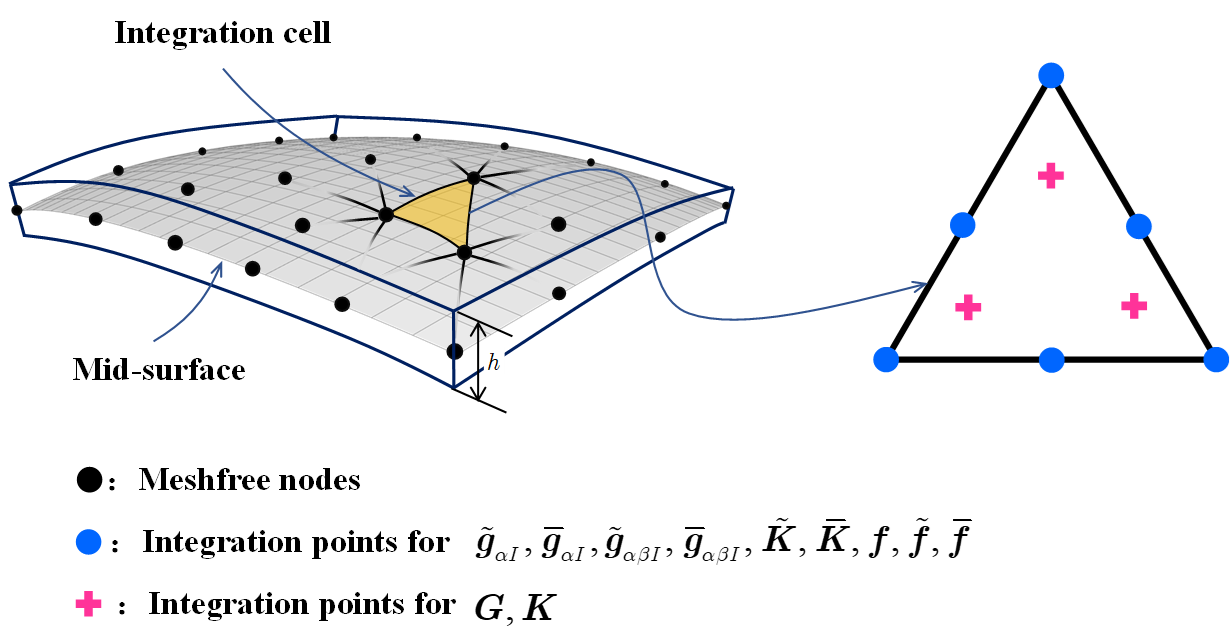
\includegraphics[width=\textwidth]{figures/2}
\caption{Integration scheme for Hu-Washizu weak form.}\label{fig2}
\end{figure}

\DIFdelbegin \DIFdel{In order to meet }\DIFdelend \DIFaddbegin \DIFadd{To satisfy }\DIFaddend the integration constraint of thin shell problem, the approximated stresses $N^{\alpha\beta h}$, $M^{\alpha\beta h}$ \DIFdelbegin \DIFdel{are assumed to be a similar form with strains, }\DIFdelend \DIFaddbegin \DIFadd{were assumed to have a comparable form to strains, and }\DIFaddend yields:
\begin{equation}\label{approxse1}
N^{\alpha\beta h}(\boldsymbol \xi) = \boldsymbol q^T(\boldsymbol \xi) \boldsymbol a^\alpha \cdot \boldsymbol d^{\beta}_N,\quad
\boldsymbol a_\alpha N^{\alpha\beta h}(\boldsymbol \xi) = \boldsymbol q^T(\boldsymbol \xi) \boldsymbol d_N^\beta
\end{equation}
\begin{equation}\label{approxse2}
    M^{\alpha\beta h}(\boldsymbol \xi) = \boldsymbol q^T(\boldsymbol \xi) \boldsymbol a_3 \cdot \boldsymbol d^{\alpha\beta}_M,\quad
    \boldsymbol a_3 M^{\alpha\beta h}(\boldsymbol \xi) = \boldsymbol q^T(\boldsymbol \xi) \boldsymbol d^{\alpha\beta}_M
\end{equation}
substituting the approximations of Eqs. (\ref{approxv}), (\ref{approxsn1}), (\ref{approxsn2}), (\ref{approxse1}), (\ref{approxse2}) into Eqs. (\ref{w3}), (\ref{w4}) can express $\boldsymbol d^\varepsilon_\beta$ and $\boldsymbol d^\kappa_{\alpha\beta}$ by $\boldsymbol d$ as:
\begin{equation}\label{depsilon}
\boldsymbol d^\varepsilon_\beta = \boldsymbol G^{-1} \left (\sum_{I=1}^{n_p}(\tilde{\boldsymbol g}_{\beta I} - \bar{\boldsymbol g}_{\beta I}) \boldsymbol d_I + \hat{\boldsymbol g}_\beta \right )
\end{equation}
\begin{equation}\label{dkappa}
\boldsymbol d^\kappa_{\alpha\beta} = \boldsymbol G^{-1} \left (\sum_{I=1}^{n_p}(\tilde{\boldsymbol g}_{\alpha\beta I} - \bar{\boldsymbol g}_{\alpha\beta I})\boldsymbol d_I + \hat{\boldsymbol g}_{\alpha\beta} \right )
\end{equation}
with
\begin{equation}
\boldsymbol G = \int_{\Omega_C} \boldsymbol q^T \boldsymbol q d\Omega
\end{equation}
\begin{subequations}\label{gn}
\begin{align}
\tilde{\boldsymbol g}_{\beta I} &= \int_{\Gamma_C} \Psi_I \boldsymbol q n_\beta d\Gamma
- \int_{\Omega_C} \Psi_I \boldsymbol q_{\vert \beta} d\Omega \\
\bar{\boldsymbol g}_{\beta I} &= \int_{\Gamma_C\cap\Gamma_v} \Psi_I \boldsymbol q n_\beta d\Gamma \\
\hat{\boldsymbol g}_{\beta} &= \int_{\Gamma_C\cap\Gamma_v} \boldsymbol q n_\beta \bar{\boldsymbol v} d\Gamma 
\end{align}
\end{subequations}
\begin{subequations}\label{gm}
\begin{align}
\small
\begin{split}
\tilde{\boldsymbol g}_{\alpha\beta I} &= \int_{\Gamma_C} \Psi_{I,\gamma}n^\gamma \boldsymbol q n_\alpha n_\beta d\Gamma 
- \int_{\Gamma_C} \Psi_I(\boldsymbol q_{\vert \beta} n_\alpha + (\boldsymbol q s_\alpha n_\beta)_{,\gamma}s^\gamma) d\Gamma \\
&+ [[\Psi_I \boldsymbol q s_\alpha n_\beta]]_{\boldsymbol x\in C_C}
- \int_{\Omega_C} \Psi \boldsymbol q_{,\alpha\vert \beta} d\Omega \\
\end{split} \\
\small
\begin{split}
\bar{\boldsymbol g}_{\alpha\beta I} &= \int_{\Gamma_C\cap\Gamma_\theta} \Psi_{I,\gamma}n^\gamma \boldsymbol q n_\alpha n_\beta d\Gamma 
- \int_{\Gamma_C\cap\Gamma_v} \Psi_I(\boldsymbol q_{\vert \beta} n_\alpha + (\boldsymbol q s_\alpha n_\beta)_{,\gamma}s^\gamma) d\Gamma \\
&+ [[\Psi_I \boldsymbol q s_\alpha n_\beta]]_{\boldsymbol x\in C_C\cap C_v}
\end{split} \\
\small
\begin{split}
\hat{\boldsymbol g}_{\alpha\beta} &= \int_{\Gamma_C\cap\Gamma_\theta} \boldsymbol q n_\alpha n_\beta \boldsymbol a_3 \bar{\theta}_{\boldsymbol n} d\Gamma 
- \int_{\Gamma_C\cap\Gamma_v}(\boldsymbol q_{\vert \beta} n_\alpha + (\boldsymbol q s_\alpha n_\beta)_{,\gamma}s^\gamma)\bar{\boldsymbol v} d\Gamma \\
&+ [[\boldsymbol q s_\alpha n_\beta \bar{\boldsymbol v}]]_{\boldsymbol x\in C_C\cap C_v}
\end{split}
\end{align}
\end{subequations}
where evaluations of $\boldsymbol q_{\vert \beta}$, $\boldsymbol q_{,\alpha\vert\beta}$ are \DIFdelbegin \DIFdel{detail }\DIFdelend \DIFaddbegin \DIFadd{discussed }\DIFaddend in \ref{derivative}. Further plugging Eqs. (\ref{depsilon}) and (\ref{dkappa}) back into Eqs. (\ref{approxsn1}) and (\ref{approxsn2}) respectively gives the final expression of $\boldsymbol v^h_{,\alpha}$, $\varepsilon^h_{\alpha\beta}$ and \DIFdelbegin \DIFdel{$-\boldsymbol v^h_{,\alpha\beta}$}\DIFdelend \DIFaddbegin \DIFadd{$-\boldsymbol v^h_{,\alpha}\vert_{\beta}$}\DIFaddend , $\boldsymbol \kappa^h_{\alpha\beta}$ as: \begin{subequations}
\begin{equation}
\boldsymbol v^h_{,\alpha} = \sum_{I=1}^{n_p}(
\tilde \Psi_{I,\alpha} - \bar \Psi_{I,\alpha}) \boldsymbol d_I +
\boldsymbol q^T \boldsymbol G^{-1}\hat{\boldsymbol g}_{\alpha}
\end{equation}
\begin{equation}\label{epsilonh}
\begin{split}
\varepsilon^h_{\alpha\beta} &= 
\sum_{I=1}^{n_p} \frac{1}{2}(\boldsymbol a_\alpha \tilde \Psi_{I,\beta} + \boldsymbol a_\beta \tilde \Psi_{I,\alpha}) \cdot \boldsymbol d_I 
- \sum_{I=1}^{n_p} \frac{1}{2}(\boldsymbol a_\alpha \bar \Psi_{I,\beta} + \boldsymbol a_\beta \bar \Psi_{I,\alpha}) \cdot \boldsymbol d_I \\
&+ \boldsymbol q^T \boldsymbol G^{-1} \frac{1}{2}(\boldsymbol a_\alpha \cdot \hat{\boldsymbol g}_{\beta} + \boldsymbol a_\beta \cdot \hat{\boldsymbol g}_{\alpha}) \\
&= \tilde \varepsilon^h_{\alpha\beta} - \bar \varepsilon^h_{\alpha\beta} + \hat \varepsilon^h_{\alpha\beta}
\end{split}
\end{equation}
\end{subequations}
\begin{subequations}
\begin{equation}
-\boldsymbol v^h_{,\alpha}\vert_\beta = \sum_{I=1}^{n_p} (
\tilde \Psi_{I,\alpha\beta} -
\bar \Psi_{I,\alpha\beta} ) \boldsymbol d_I +
\boldsymbol q^T \boldsymbol G^{-1}\hat{\boldsymbol g}_{\alpha\beta}
\end{equation}
\begin{equation}\label{kappah}
\begin{split}
\kappa^h_{\alpha\beta} &= \sum_{I=1}^{n_p} \tilde \Psi_{I,\alpha\beta} \boldsymbol a_3 \cdot \boldsymbol d_I
- \sum_{I=1}^{n_p} \bar \Psi_{I,\alpha\beta} \boldsymbol a_3 \cdot \boldsymbol d_I +
\boldsymbol q^T \boldsymbol G^{-1}\boldsymbol a_3 \cdot \hat{\boldsymbol g}_{\alpha\beta} \\
&= \tilde \kappa^h_{\alpha\beta} - \bar \kappa^h_{\alpha\beta} + \hat \kappa^h_{\alpha\beta}
\end{split}
\end{equation}
\end{subequations}
with
\begin{equation}\label{epsilon2}
\left \{
\begin{split}
\tilde \varepsilon^h_{\alpha\beta} &= \sum_{I=1}^{n_p} \frac{1}{2}(\boldsymbol a_\alpha \tilde \Psi_{I,\beta} + \boldsymbol a_\beta \tilde \Psi_{I,\alpha}) \cdot \boldsymbol d_I
=\sum_{I=1}^{n_p} \tilde{\boldsymbol \varepsilon}_{\alpha\beta I} \cdot \boldsymbol d_I \\
\bar \varepsilon^h_{\alpha\beta} &= \sum_{I=1}^{n_p} \frac{1}{2}(\boldsymbol a_\alpha \bar \Psi_{I,\beta} + \boldsymbol a_\beta \bar \Psi_{I,\alpha}) \cdot \boldsymbol d_I
=\sum_{I=1}^{n_p} \bar{\boldsymbol \varepsilon}_{\alpha\beta I} \cdot \boldsymbol d_I \\
\hat \varepsilon^h_{\alpha\beta} &= \boldsymbol q^T \boldsymbol G^{-1} \frac{1}{2}(\boldsymbol a_\alpha\cdot\hat{\boldsymbol g}_\beta + \boldsymbol a_\beta \cdot \hat{\boldsymbol g}_\alpha)
\end{split}
\right .
\end{equation}
\begin{equation}
\left \{
\begin{split}
&\tilde{\Psi}_{I,\alpha}(\boldsymbol \xi) = \boldsymbol q^T(\boldsymbol \xi) \boldsymbol G^{-1} \tilde{\boldsymbol g}_{\alpha I} \\
&\bar{\Psi}_{I,\alpha}(\boldsymbol \xi) = \boldsymbol q^T(\boldsymbol \xi) \boldsymbol G^{-1} \bar{\boldsymbol g}_{\alpha I} \\
&\tilde{\boldsymbol \varepsilon}_{\alpha\beta I} = \frac{1}{2}(\boldsymbol a_\alpha \tilde \Psi_{I,\beta} + \boldsymbol a_\beta \tilde \Psi_{I,\alpha}) \\
&\bar{\boldsymbol \varepsilon}_{\alpha\beta I} = \frac{1}{2}(\boldsymbol a_\alpha \bar \Psi_{I,\beta} + \boldsymbol a_\beta \bar \Psi_{I,\alpha})
\end{split}
\right .
\end{equation}
\begin{equation}\label{kappa2}
\left \{
\begin{split}
\tilde \kappa^h_{\alpha\beta} &= \sum_{I=1}^{n_p} \tilde \Psi_{I,\alpha\beta}\boldsymbol a_3 \cdot \boldsymbol d_I 
= \sum_{I = 1}^{n_p} \tilde{\boldsymbol \kappa}_{\alpha\beta I} \cdot \boldsymbol d_I\\
\bar \kappa^h_{\alpha\beta} &= \sum_{I=1}^{n_p} \bar \Psi_{I,\alpha\beta}\boldsymbol a_3 \cdot \boldsymbol d_I
= \sum_{I = 1}^{n_p} \bar{\boldsymbol \kappa}_{\alpha\beta I} \cdot \boldsymbol d_I \\
\hat \kappa^h_{\alpha\beta} &= \boldsymbol q^T \boldsymbol G^{-1} \boldsymbol a_3 \cdot \hat{\boldsymbol g}_{\alpha\beta}
\end{split}
\right .
\end{equation}
\begin{equation}
\left \{
\begin{split}
&\tilde{\Psi}_{I,\alpha\beta}(\boldsymbol \xi) = \boldsymbol q^T(\boldsymbol \xi) \boldsymbol G^{-1} \tilde{\boldsymbol g}_{\alpha\beta I} \\
&\bar{\Psi}_{I,\alpha\beta}(\boldsymbol \xi) = \boldsymbol q^T(\boldsymbol \xi) \boldsymbol G^{-1} \tilde{\boldsymbol g}_{\alpha\beta I} \\
&\tilde{\boldsymbol \kappa}_{\alpha\beta I} = \tilde \Psi_{I,\alpha\beta}\boldsymbol a_3 \\
&\bar {\boldsymbol \kappa}_{\alpha\beta I} = \bar \Psi_{I,\alpha\beta}\boldsymbol a_3 \\
\end{split}
\right .
\end{equation}

% Furthermore, taking Eqs. (\ref{approxsn1}) and (\ref{approxsn2}) into Eqs.(\ref{w1}) and (\ref{w2}) can obtain the approximated effective stresses $N^{\alpha\beta h}$, $M^{\alpha\beta h}$ and their coefficients $\boldsymbol d_N^\beta$, $\boldsymbol d_M^{\alpha\beta}$ as:
% \begin{equation}\label{d_N1}
%  \delta \boldsymbol d^\varepsilon_\alpha \cdot \boldsymbol G^{\alpha\eta}_N \cdot \boldsymbol d^\varepsilon_\eta = \delta \boldsymbol d^\varepsilon_\alpha \cdot \boldsymbol d_N^\alpha \boldsymbol G \quad\Rightarrow \quad & \boldsymbol d_N^\alpha = \boldsymbol G^{-1} \boldsymbol G_N^{\alpha\eta} \cdot \boldsymbol d^\varepsilon_\eta
% \end{equation}
% \begin{equation}\label{d_M1}
%  \delta \boldsymbol d^\kappa_{\alpha\beta} : \boldsymbol G_M^{\alpha\beta\gamma\eta} : \boldsymbol d^\kappa_{\gamma\eta} \boldsymbol G = \delta \boldsymbol d^\kappa_{\alpha\beta} \cdot \boldsymbol d_M^{\alpha\beta} \boldsymbol G \\
% \Rightarrow \; \boldsymbol d_M^{\alpha\beta} = \boldsymbol G^{-1} \boldsymbol G_{\alpha\beta}^M \cdot \boldsymbol d^\kappa_{\gamma\eta}
% \end{equation}
% with
% \begin{equation}
% \boldsymbol G^{\alpha\eta}_N = \int_{\Omega_C} \boldsymbol a_\beta hC^{\alpha\beta\gamma\eta} \boldsymbol a_\gamma \boldsymbol q \boldsymbol q^T d\Omega
% \end{equation}
% \begin{equation}
% \boldsymbol G^{\alpha\beta\gamma\eta}_M = \int_{\Omega_C} \boldsymbol a_3 \frac{h^3}{12}C^{\alpha\beta\gamma\eta}\boldsymbol a_3 \boldsymbol q\boldsymbol q^T d\Omega
% \end{equation}
%  
% Finally, taking Eqs. (\ref{d_N1}) and (\ref{d_M1}) back to Eqs. (\ref{approxse1}), (\ref{approxse2}) can express the components of stresses as follows:
% \begin{equation}\label{Nh}
% N^{\alpha\beta h} = \boldsymbol q^T \boldsymbol G^{-1}\frac{1}{2}(\boldsymbol a^\alpha \cdot \boldsymbol G^{\beta\gamma}_{N} + \boldsymbol a^\beta \cdot \boldsymbol G^{\alpha\gamma}_N) \cdot \boldsymbol d^{\varepsilon}_\gamma
% \end{equation}
% \begin{equation}\label{Mh}
% M^{\alpha\beta h} = \boldsymbol q^T \boldsymbol G^{-1} \boldsymbol a_3 \cdot \boldsymbol G^{\alpha\beta\gamma\eta}_M \cdot \boldsymbol d^\kappa_{\gamma\eta}
% \end{equation}

It has to be noted that, referring to reproducing kernel gradient smoothing framework \cite{wang2019a}, $\tilde \Psi_{I,\alpha}$, $\tilde \Psi_{I,\alpha\beta}$ are actually the first and second order smoothed gradients in curvilinear coordinates.\DIFdelbegin \DIFdel{$\tilde{\boldsymbol g}_{\alpha I}$ and $\tilde{\boldsymbol g}_{\alpha \beta I}$ are }\DIFdelend \DIFaddbegin \DIFadd{If }\DIFaddend the right hand side integration constraints for first and second order gradients \DIFdelbegin \DIFdel{, }\DIFdelend \DIFaddbegin \DIFadd{are $\tilde{\boldsymbol g}_{\alpha I}$ and $\tilde{\boldsymbol g}_{\alpha \beta I}$, respectively, }\DIFaddend then this formulation can \DIFdelbegin \DIFdel{meet }\DIFdelend \DIFaddbegin \DIFadd{satisfy  }\DIFaddend the variational consistency for the \DIFdelbegin \DIFdel{$p$-th }\DIFdelend \DIFaddbegin \DIFadd{second }\DIFaddend order polynomials. It should be \DIFdelbegin \DIFdel{known that , }\DIFdelend \DIFaddbegin \DIFadd{mentioned that }\DIFaddend in curved model, the variational consistency for non-polynomial functions, \DIFdelbegin \DIFdel{like }\DIFdelend \DIFaddbegin \DIFadd{such as }\DIFaddend trigonometric functions, should be required for the polynomial solution. Even with \DIFdelbegin \DIFdel{$p$-th order }\DIFdelend \DIFaddbegin \DIFadd{high order polynomial }\DIFaddend variational consistency, the proposed formulation \DIFdelbegin \DIFdel{can not }\DIFdelend \DIFaddbegin \DIFadd{cannot }\DIFaddend exactly reproduce the solution spanned by \DIFaddbegin \DIFadd{the }\DIFaddend basis functions. However, the accuracy of reproducing kernel smoothed gradients is still \DIFdelbegin \DIFdel{better that }\DIFdelend \DIFaddbegin \DIFadd{superior than the }\DIFaddend traditional meshfree formulation. \DIFdelbegin \DIFdel{Numerical }\DIFdelend \DIFaddbegin \DIFadd{The numerical }\DIFaddend examples in the \DIFdelbegin \DIFdel{section below will provide better evidence to prove the accuracy }\DIFdelend \DIFaddbegin \DIFadd{following section will better demonstrate the precision }\DIFaddend of the reproducing kernel smoothed gradients.


\section{Naturally variational enforcement for essential boundary conditions}\label{boundary}
\subsection{Discrete equilibrium equations}
With the approximated effective stresses and strains, the last equation of weak form Eq. (\ref{w5}) becomes:
\begin{equation}\label{w51}
- \sum_{C=1}^{n_e}\sum_{I=1}^{n_p} \delta \boldsymbol d_I \cdot \left ( (\tilde{\boldsymbol g}^T_{\alpha I} - \bar{\boldsymbol g}^T_{\alpha I}) \boldsymbol d_N^{\alpha}
+ (\tilde{\boldsymbol g}^T_{\alpha\beta I} - \bar{\boldsymbol g}^T_{\alpha\beta I}) \boldsymbol d_M^{\alpha\beta} \right ) = - \sum_{I=1}^{n_p}\delta d_I \cdot \boldsymbol f_I
\end{equation}
where $\boldsymbol f_I$'s are the components of the traditional force vector:
\begin{equation}
        \boldsymbol f_I = \int_{\Gamma_t} \Psi_I \bar{\boldsymbol t} d\Gamma - \int_{\Gamma_M} \Psi_{I,\gamma} n^\gamma \bar M_{\boldsymbol{nn}} d\Gamma + [[\Psi_I\boldsymbol a_3 \bar P]]_{\boldsymbol x\in C_P} + \int_\Omega \Psi_I \bar{\boldsymbol b} d\Omega
\end{equation}
The left side of Eq. (\ref{w51}) can be simplified using the following steps. For clarity, the derivation of first term in Eq. (\ref{w51}) taken as an example is given by:
\begin{equation}
\begin{split}
\sum_{I=1}^{n_p} \delta \boldsymbol d_I \cdot \tilde{\boldsymbol g}^T_{\alpha I} \boldsymbol d_N^\alpha 
&= \sum_{I=1}^{n_p} \delta \boldsymbol d_I \cdot (\boldsymbol G^{-1} \tilde{\boldsymbol g}_{\alpha I})^T  \boldsymbol G \boldsymbol d^\alpha_N \\
&= \int_{\Omega_C} \sum_{I=1}^{n_p} \delta \boldsymbol d_I \cdot (\boldsymbol q^T\boldsymbol G^{-1} \tilde{\boldsymbol g}_{\alpha I})^T  \boldsymbol q^T \boldsymbol d^\alpha_N d\Omega \\
&= \int_{\Omega_C} \sum_{I=1}^{n_p} \delta \boldsymbol d_I \cdot \boldsymbol a_\beta(\boldsymbol q^T\boldsymbol G^{-1} \tilde{\boldsymbol g}_{\alpha I})^T  N^{\alpha\beta h} d\Omega \\
& = \int_{\Omega_C} \delta \tilde \varepsilon_{\alpha\beta}^h N^{\alpha\beta h} d\Omega 
\end{split}
\end{equation}
following the above procedure and including the weak form of Eqs. (\ref{w1}), (\ref{w2}), the left side of Eq. (\ref{w51}) in $\Omega_C$ becomes:
\begin{equation}
\begin{split}
&\sum_{I=1}^{n_p} \delta \boldsymbol d_I \cdot  \left ( 
(\tilde{\boldsymbol g}^T_{\alpha I} - \bar{\boldsymbol g}^T_{\alpha I}) \boldsymbol d^\alpha_N
+(\tilde{\boldsymbol g}^T_{\alpha\beta I} - \bar{\boldsymbol g}^T_{\alpha\beta I}) \boldsymbol d^{\alpha\beta}_M \right) \\
=& \int_{\Omega_C}\left ( (\delta \tilde \varepsilon^h_{\alpha\beta} - \delta \bar \varepsilon^h_{\alpha\beta}) N^{\alpha\beta h}
+ (\delta \tilde \kappa^h_{\alpha\beta} - \delta \bar \kappa^h_{\alpha\beta})M^{\alpha\beta h}
\right ) d\Omega \\
= &\int_{\Omega_C} (\delta \tilde \varepsilon^h_{\alpha\beta} - \delta \bar \varepsilon^h_{\alpha\beta}) hC^{\alpha\beta\gamma\eta} \varepsilon^h_{\gamma\eta}
+ (\delta \tilde \kappa^h_{\alpha\beta} - \delta \bar \kappa^h_{\alpha\beta}) \frac{h^3}{12}C^{\alpha\beta\gamma\eta}\kappa^h_{\gamma\eta} \\
= &\int_{\Omega_C}\delta \tilde \varepsilon^h_{\alpha\beta}hC^{\alpha\beta\gamma\eta} \tilde\varepsilon^h_{\gamma\eta} d\Omega
+ \int_{\Omega_C}\delta \tilde \kappa^h_{\alpha\beta} \frac{h^3}{12}C^{\alpha\beta\gamma\eta}\tilde \kappa^h_{\gamma\eta}d\Omega \\
- &\int_{\Omega_C}\delta \tilde \varepsilon^h_{\alpha\beta}hC^{\alpha\beta\gamma\eta} \bar \varepsilon^h_{\gamma\eta} d\Omega
- \int_{\Omega_C}\delta \bar \varepsilon^h_{\alpha\beta}hC^{\alpha\beta\gamma\eta} \tilde \varepsilon^h_{\gamma\eta} d\Omega \\
- &\int_{\Omega_C}\delta \tilde \kappa^h_{\alpha\beta} \frac{h^3}{12}C^{\alpha\beta\gamma\eta}\bar \kappa^h_{\gamma\eta}d\Omega 
- \int_{\Omega_C}\delta \bar \kappa^h_{\alpha\beta} \frac{h^3}{12}C^{\alpha\beta\gamma\eta}\tilde \kappa^h_{\gamma\eta}d\Omega \\
+ &\int_{\Omega_C}\delta \bar \varepsilon^h_{\alpha\beta}hC^{\alpha\beta\gamma\eta} \bar \varepsilon^h_{\gamma\eta} d\Omega
+ \int_{\Omega_C}\delta \bar \kappa^h_{\alpha\beta} \frac{h^3}{12}C^{\alpha\beta\gamma\eta}\bar \kappa^h_{\gamma\eta}d\Omega \\
+ &\int_{\Omega_C}(\delta \tilde \varepsilon^h_{\alpha\beta} - \delta \bar \varepsilon^h_{\alpha\beta})hC^{\alpha\beta\gamma\eta} \hat \varepsilon^h_{\gamma\eta} d\Omega
+ \int_{\Omega_C}(\delta \tilde \kappa^h_{\alpha\beta} - \delta \bar \kappa^h_{\alpha\beta})\frac{h^3}{12}C^{\alpha\beta\gamma\eta}\hat \kappa^h_{\gamma\eta}d\Omega \\
\end{split}
\end{equation}
on further substituting Eqs. (\ref{epsilon2}) and (\ref{kappa2}) into above equation gives the final discrete equilibrium equations, respectively: 
\begin{equation}
        (\boldsymbol K + \tilde{\boldsymbol K} + \bar{\boldsymbol K} )\boldsymbol d = \boldsymbol f + \tilde{\boldsymbol f} + \bar{\boldsymbol f}
\end{equation}
where
\begin{equation}\label{de1}
        \boldsymbol K_{IJ} = \int_\Omega \tilde{\boldsymbol \varepsilon}_{\alpha\beta I} hC^{\alpha\beta\gamma\eta}\tilde{\boldsymbol \varepsilon}_{\gamma\eta J} d\Omega + \int_\Omega \tilde{\boldsymbol \kappa}_{\alpha\beta I} \frac{h^3}{12}C^{\alpha\beta\gamma\eta} \tilde{\boldsymbol \kappa}_{\alpha\beta J} d\Omega
\end{equation}
\begin{subequations}\label{de2}
\begin{align}
\begin{split}
        \tilde{\boldsymbol K}_{IJ} = &- \int_{\Gamma_v} (\Psi_I \tilde{\boldsymbol T}_{NJ} + \tilde{\boldsymbol T}_{NJ} \Psi_J) d\Gamma \\
                                     &+ \int_{\Gamma_\theta} (\Psi_{I,\gamma} n^\gamma \boldsymbol a_3 \tilde{\boldsymbol M}_{\boldsymbol{nn}J} + \boldsymbol a_3 \tilde{\boldsymbol M}_{\boldsymbol{nn}I} \Psi_{I,\gamma}n^\gamma)d\Gamma \\
                                     & + ([[\Psi_I \boldsymbol a_3 \tilde{\boldsymbol P}_J]] + [[\tilde{\boldsymbol P}_I \boldsymbol a_3 \Psi_J]])_{\boldsymbol x \in C_v}
\end{split} \\
\tilde{\boldsymbol f}_I = &- \int_{\Gamma_v} \tilde{\boldsymbol T}_{NI} \cdot \bar{\boldsymbol v} d\Gamma + \int_{\Gamma_\theta} \tilde{\boldsymbol M}_{\boldsymbol{nn}I} \bar{\theta}_{\boldsymbol n} d\Gamma + [[\tilde{\boldsymbol P}_I\boldsymbol a_3 \cdot \bar{\boldsymbol v}]]_{\boldsymbol x \in C_v}
\end{align}
\end{subequations}
\begin{subequations}\label{de3}
\begin{align}
\bar{\boldsymbol K}_{IJ} &= - \int_{\Gamma_v} \bar{\boldsymbol T}_{MI} \Psi_J d\Gamma 
+ \int_{\Gamma_\theta} \boldsymbol a_3\bar{\boldsymbol M}_{\boldsymbol{nn}I} \Psi_{J,\gamma}n^\gamma d\Gamma + [[\bar{\boldsymbol P}_I \boldsymbol a_3 \Psi_J]]_{\boldsymbol x \in C_v} \\
\bar{\boldsymbol f}_I &= - \int_{\Gamma_v} \bar{\boldsymbol T}_{MI} \cdot \bar{\boldsymbol v} d\Gamma + \int_{\Gamma_\theta} \bar{\boldsymbol M}_{\boldsymbol{nn} I} \bar{\theta}_{\boldsymbol n} d\Gamma + [[\bar{\boldsymbol P}_I\boldsymbol a_3 \cdot \bar{\boldsymbol v}]]_{\boldsymbol x \in C_v}
\end{align}
\end{subequations}

The detailed derivations of Eqs (\ref{de1})-(\ref{de3}) are listed in the \ref{derivations}. As shown in these equations, Eq. (\ref{de1}) is the conventional stiffness matrix evaluated by smoothed gradients $\tilde \Psi_{I,\alpha}$, $\tilde \Psi_{I,\alpha}\vert_\beta$, and the Eqs. (\ref{de2}) and (\ref{de3}) contribute for the enforcement of essential boundary. It should be mentioned that, in accordance with reproducing kernel smoothed gradient framework, the integration scheme of Eqs. (\ref{de1}-\ref{de3}) should be aligned with the those used in the construction of smoothed gradients. The integration scheme used for proposed method is shown in Fig. \ref{fig2}, \DIFdelbegin \DIFdel{the }\DIFdelend \DIFaddbegin \DIFadd{in which the total number of the blue circular integration points has been optimized from a global point of view, aiming to reduce the computation of traditional meshfree shape functions and its first order derivatives. In contrast, for assembly stiffness matrix $\boldsymbol K$, the low order Gauss integration rule is suitable to ensure the accuracy due to the inherently variational consistency in smoothed gradients. The }\DIFaddend detailed positions and weight of integration points \DIFaddbegin \DIFadd{and the efficiency demonstration of this optimized integration scheme }\DIFaddend can be found in \DIFdelbegin \DIFdel{\mbox{%DIFAUXCMD
\cite{du2022}  }\hskip0pt%DIFAUXCMD
}\DIFdelend \DIFaddbegin \DIFadd{\mbox{%DIFAUXCMD
\cite{wang2019a, du2022}  }\hskip0pt%DIFAUXCMD
}\DIFaddend With a close look at Eqs. (\ref{de2}) and (\ref{de3}), the proposed approach for enforcing essential boundary conditions show an identical structure with traditional Nitsche's method, both have the consistent and stabilized terms. So, the next subsection will review the Nitsche's method and compare it with the proposed method.

\subsection{Comparison with Nitsche's method}
The Nitsche's method for enforcing essential boundaries can be regarded as a combination of Lagrangian multiplier method and penalty method, in which the Lagrangian multiplier is represented by the approximated displacement. The corresponding total potential energy functional $\Pi_P$ is given by:
\DIFdelbegin \begin{displaymath}
\begin{split}
\DIFdel{\Pi_P(\boldsymbol v) }&\DIFdel{= \int_\Omega \frac{1}{2}\varepsilon_{\alpha\beta} N^{\alpha\beta} d\Omega +
\int_\Omega \frac{1}{2} \kappa_{\alpha\beta}M^{\alpha\beta} d\Omega }\\
                     &\DIFdel{- \int_{\Gamma_t} \boldsymbol v \cdot \bar{\boldsymbol t} d\Gamma 
                     + \int_{\Gamma_M} \boldsymbol v_{,\gamma} n^\gamma \boldsymbol a_3 M_{\boldsymbol{nn}} d\Gamma
                     + (\boldsymbol v \cdot \boldsymbol a_3 P)_{\boldsymbol x \in C_P}
                     - \int_\Omega \boldsymbol v \cdot \bar{\boldsymbol b} d\Omega }\\
                     &\DIFdel{- \underbrace{\int_{\Gamma_v} \boldsymbol t \cdot (\boldsymbol v - \bar{\boldsymbol v}) d\Gamma
                     + \int_{\Gamma_\theta} M_{\boldsymbol{nn}}(\theta_{\boldsymbol n} - \bar \theta_{\boldsymbol n})d\Gamma
                     + (P\boldsymbol a_3 \cdot (\boldsymbol v - \bar{\boldsymbol v}))_{\boldsymbol x \in C_v}}_{\text{consistent term}} }\\
                     &\DIFdel{+ \underbrace{\frac{\alpha_v}{2} \int_{\Gamma_v} \boldsymbol v \cdot \boldsymbol v d\Gamma 
                     + \frac{\alpha_\theta}{2} \int_{\Gamma_\theta} \theta_{\boldsymbol n}^2 d\Gamma
             + \frac{\alpha_C}{2}(\boldsymbol v \cdot \boldsymbol v)_{\boldsymbol x\in C_v}}_{\text{stabilized term}}
}\end{split}
\DIFdel{}\end{displaymath}%DIFAUXCMD
\DIFdelend \DIFaddbegin \begin{equation}
\begin{split}
\DIFadd{\Pi_P(\boldsymbol v) }&\DIFadd{= \int_\Omega \frac{1}{2}\varepsilon_{\alpha\beta} N^{\alpha\beta} d\Omega +
\int_\Omega \frac{1}{2} \kappa_{\alpha\beta}M^{\alpha\beta} d\Omega }\\
                     &\DIFadd{- \int_{\Gamma_t} \boldsymbol v \cdot \bar{\boldsymbol t} d\Gamma 
                     + \int_{\Gamma_M} \boldsymbol v_{,\gamma} n^\gamma \boldsymbol a_3 M_{\boldsymbol{nn}} d\Gamma
                     + (\boldsymbol v \cdot \boldsymbol a_3 P)_{\boldsymbol x \in C_P}
                     - \int_\Omega \boldsymbol v \cdot \bar{\boldsymbol b} d\Omega }\\
                     &\DIFadd{- \underbrace{\int_{\Gamma_v} \boldsymbol t \cdot (\boldsymbol v - \bar{\boldsymbol v}) d\Gamma
                     + \int_{\Gamma_\theta} M_{\boldsymbol{nn}}(\theta_{\boldsymbol n} - \bar \theta_{\boldsymbol n})d\Gamma
                     + (P\boldsymbol a_3 \cdot (\boldsymbol v - \bar{\boldsymbol v}))_{\boldsymbol x \in C_v}}_{\text{consistent term}} }\\
                     &\DIFadd{+ \underbrace{\sum_{i=1}^3\frac{\alpha_{vi}}{2} \int_{\Gamma_v} \boldsymbol v \cdot \boldsymbol v d\Gamma 
                     + \frac{\alpha_\theta}{2} \int_{\Gamma_\theta} \theta_{\boldsymbol n}^2 d\Gamma
             + \frac{\alpha_C}{2}(\boldsymbol v \cdot \boldsymbol a_3)^2_{\boldsymbol x\in C_v}}_{\text{stabilized term}}
}\end{split}
\DIFadd{}\end{equation}\DIFaddend 
where the consistent term generated from the Lagrangian multiplier method contributes to enforce the essential boundary, and meet the variational consistency condition. However, the consistent term can not always ensure the coercivity of stiffness, so the penalty method is introduced to serve as a stabilized term\DIFaddbegin \DIFadd{, in which $\alpha_{vi}$'s, $\alpha_\theta$ and $\alpha_C$ are experimental artificial parameters in penalty method}\DIFaddend . With a standard variational argument, the corresponding weak form can be stated as:
\DIFdelbegin \begin{displaymath}
\begin{split}
\DIFdel{\delta \Pi_P(\boldsymbol v) }&\DIFdel{= \int_\Omega\delta \varepsilon_{\alpha\beta} N^{\alpha\beta} d\Omega +
\int_\Omega \delta \kappa_{\alpha\beta}M^{\alpha\beta} d\Omega }\\
                     &\DIFdel{- \int_{\Gamma_t} \delta \boldsymbol v \cdot \bar{\boldsymbol t} d\Gamma 
                     + \int_{\Gamma_M} \delta \boldsymbol v_{,\gamma} n^\gamma \boldsymbol a_3 M_{\boldsymbol{nn}} d\Gamma
                     + (\delta \boldsymbol v \cdot \boldsymbol a_3 P)_{\boldsymbol x \in C_P}
                     - \int_\Omega \delta \boldsymbol v \cdot \bar{\boldsymbol b} d\Omega }\\
                     &\DIFdel{- \int_{\Gamma_v} \delta \boldsymbol v \cdot \boldsymbol t d\Gamma 
                     + \int_{\Gamma_\theta} \delta \theta_{\boldsymbol n} M_{\boldsymbol{nn}}d\Gamma 
                     + (\boldsymbol v \cdot \boldsymbol a_3 P)_{\boldsymbol x \in C_v}}\\
                     &\DIFdel{- \int_{\Gamma_v} \delta \boldsymbol t \cdot (\boldsymbol v - \bar{\boldsymbol v}) d\Gamma
                     + \int_{\Gamma_\theta} \delta M_{\boldsymbol{nn}}(\theta_{\boldsymbol n} - \bar \theta_{\boldsymbol n})d\Gamma
                     + (\delta P\boldsymbol a_3 \cdot (\boldsymbol v - \bar{\boldsymbol v}))_{\boldsymbol x \in C_v} }\\
                     &\DIFdel{+ \alpha_v \int_{\Gamma_v} \delta \boldsymbol v \cdot \boldsymbol v d\Gamma 
                     + \alpha_\theta \int_{\Gamma_\theta} \delta \theta_{\boldsymbol n}\theta_{\boldsymbol n} d\Gamma
                     + \alpha_C(\delta \boldsymbol v \cdot \boldsymbol v)_{\boldsymbol x\in C_v} }\\
                     &\DIFdel{= 0
}\end{split}
\DIFdel{}\end{displaymath}%DIFAUXCMD
\DIFdelend \DIFaddbegin \begin{equation}
\begin{split}
\DIFadd{\delta \Pi_P(\boldsymbol v) }&\DIFadd{= \int_\Omega\delta \varepsilon_{\alpha\beta} N^{\alpha\beta} d\Omega +
\int_\Omega \delta \kappa_{\alpha\beta}M^{\alpha\beta} d\Omega }\\
                     &\DIFadd{- \int_{\Gamma_t} \delta \boldsymbol v \cdot \bar{\boldsymbol t} d\Gamma 
                     + \int_{\Gamma_M} \delta \boldsymbol v_{,\gamma} n^\gamma \boldsymbol a_3 M_{\boldsymbol{nn}} d\Gamma
                     + (\delta \boldsymbol v \cdot \boldsymbol a_3 P)_{\boldsymbol x \in C_P}
                     - \int_\Omega \delta \boldsymbol v \cdot \bar{\boldsymbol b} d\Omega }\\
                     &\DIFadd{- \int_{\Gamma_v} \delta \boldsymbol v \cdot \boldsymbol t d\Gamma 
                     + \int_{\Gamma_\theta} \delta \theta_{\boldsymbol n} M_{\boldsymbol{nn}}d\Gamma 
                     + (\boldsymbol v \cdot \boldsymbol a_3 P)_{\boldsymbol x \in C_v}}\\
                     &\DIFadd{- \int_{\Gamma_v} \delta \boldsymbol t \cdot (\boldsymbol v - \bar{\boldsymbol v}) d\Gamma
                     + \int_{\Gamma_\theta} \delta M_{\boldsymbol{nn}}(\theta_{\boldsymbol n} - \bar \theta_{\boldsymbol n})d\Gamma
                     + (\delta P\boldsymbol a_3 \cdot (\boldsymbol v - \bar{\boldsymbol v}))_{\boldsymbol x \in C_v} }\\
                     &\DIFadd{+ \sum_{i=1}^{3}\alpha_{vi} \int_{\Gamma_v} (\delta \boldsymbol v \cdot \boldsymbol a_i) (\boldsymbol a_i \cdot \boldsymbol v) d\Gamma 
                     + \alpha_\theta \int_{\Gamma_\theta} \delta \theta_{\boldsymbol n}\theta_{\boldsymbol n} d\Gamma
                     + \alpha_C(\delta \boldsymbol v \cdot \boldsymbol a_3 \; \boldsymbol a_3 \cdot \boldsymbol v)_{\boldsymbol x\in C_v} }\\
                     &\DIFadd{= 0
}\end{split}
\DIFadd{}\end{equation}\DIFaddend 
\DIFdelbegin \DIFdel{in which $\alpha_v$, $\alpha_\theta$ and $\alpha_C$ represent experimental artificial parameters. }\DIFdelend Further invoking the conventional reproducing kernel approximation of Eq. (\ref{approxv}) leads to the following discrete equilibrium equations:
\begin{equation}
\sum_{J=1}^{n_p}(\boldsymbol K_{IJ} + \boldsymbol K^c_{IJ} + \boldsymbol K^s_{IJ}) \boldsymbol d_J = \boldsymbol f_I + \boldsymbol f^c + \boldsymbol f^s
\end{equation}
where the stiffness $\boldsymbol K_{IJ}$ is identical with Eq. (\ref{de1}). $\boldsymbol K^c_{IJ}$ and $\boldsymbol K^s_{IJ}$ are the stiffness matrices for consistent and stabilized terms, respectively, and have the following form:
\begin{subequations}\label{nde2}
\begin{align}
\begin{split}
\boldsymbol K^c_{IJ} = &- \int_{\Gamma_v} (\Psi_I \boldsymbol T_{NJ} + \boldsymbol T_{NJ} \Psi_J) d\Gamma \\
                                     &+ \int_{\Gamma_\theta} (\Psi_{I,\gamma} n^\gamma \boldsymbol a_3 \boldsymbol M_{\boldsymbol{nn}J} + \boldsymbol a_3 \boldsymbol M_{\boldsymbol{nn}I} \Psi_{I,\gamma}n^\gamma)d\Gamma \\
                                     & + ([[\Psi_I \boldsymbol a_3 \boldsymbol P_J]] + [[\boldsymbol P_I \boldsymbol a_3 \Psi_J]])_{\boldsymbol x \in C_v}
\end{split} \\
\boldsymbol f^c_I = &- \int_{\Gamma_v} \boldsymbol T_I \cdot \bar{\boldsymbol v} d\Gamma + \int_{\Gamma_\theta} \boldsymbol M_{\boldsymbol{nn}I} \bar{\theta}_{\boldsymbol n} d\Gamma + [[\boldsymbol P_I\boldsymbol a_3 \cdot \bar{\boldsymbol v}]]_{\boldsymbol x \in C_v}
\end{align}
\end{subequations}
\begin{subequations}\label{nde3}
\DIFdelbegin \begin{align*}
\DIFdel{\boldsymbol K^s_{IJ} }&\DIFdel{= \alpha_v \int_{\Gamma_v} \Psi_I \Psi_J \boldsymbol 1 d\Gamma 
+ \alpha_\theta \int_{\Gamma_\theta} \Psi_{I,\eta} n^\eta \boldsymbol a_3 \boldsymbol a_3 n^\gamma\Psi_{J,\gamma} d\Gamma + \alpha_C }[[\DIFdel{\Psi_I \boldsymbol a_3 \boldsymbol a_3 \Psi_J}]]\DIFdel{_{\boldsymbol x \in C_v} }\\
\DIFdel{\boldsymbol f^s_I }&\DIFdel{= \alpha_v \int_{\Gamma_v} \Psi_I \bar{\boldsymbol v} d\Gamma + \alpha_\theta \int_{\Gamma_\theta} \Psi_{I,\eta} n^\eta \boldsymbol a_3 \boldsymbol \bar \theta_{\boldsymbol n} d\Gamma + \alpha_C }[[\DIFdel{\Psi_I \boldsymbol a_3 \boldsymbol a_3 \cdot \bar{\boldsymbol v}}]]\DIFdel{_{\boldsymbol x \in C_v}
}\end{align*}%DIFAUXCMD
\DIFdelend \DIFaddbegin \begin{align}
\DIFadd{\boldsymbol K^s_{IJ} }&\DIFadd{= \boldsymbol \alpha_v \int_{\Gamma_v} \Psi_I \Psi_J d\Gamma 
+ \alpha_\theta \int_{\Gamma_\theta} \Psi_{I,\eta} n^\eta \boldsymbol a_3 \boldsymbol a_3 n^\gamma\Psi_{J,\gamma} d\Gamma + \alpha_C }[[\DIFadd{\Psi_I \boldsymbol a_3 \boldsymbol a_3 \Psi_J}]]\DIFadd{_{\boldsymbol x \in C_v} }\\
\DIFadd{\boldsymbol f^s_I }&\DIFadd{= \boldsymbol \alpha_v \int_{\Gamma_v} \Psi_I \bar{\boldsymbol v} d\Gamma + \alpha_\theta \int_{\Gamma_\theta} \Psi_{I,\eta} n^\eta \boldsymbol a_3 \boldsymbol \bar \theta_{\boldsymbol n} d\Gamma + \alpha_C }[[\DIFadd{\Psi_I \boldsymbol a_3 \boldsymbol a_3 \cdot \bar{\boldsymbol v}}]]\DIFadd{_{\boldsymbol x \in C_v}
}\end{align}\DIFaddend 
\end{subequations}
\DIFaddbegin \DIFadd{with
}\begin{equation}
\DIFadd{\boldsymbol \alpha_v = \begin{bmatrix}
    \alpha_{v1} & 0 & 0 \\
    0 & \alpha_{v2} & 0 \\
    0 & 0 & \alpha_{v3} \\
\end{bmatrix}
}\end{equation}
\DIFaddend 

On comparing with the consistent terms of Eqs. (\ref{de2}) and (\ref{nde2}), the expressions were almost identical, the major difference is that the higher order derivatives of shape functions have been replaced by smoothed gradients. Owing to the reproducing kernel framework, the construction of smoothed gradients only concerned about the computation of traditional meshfree shape functions and their first order derivatives, which avoid the costly computation of higher order derivatives. Moreover, the stabilized terms in Eq. (\ref{nde3}) employs the penalty method \DIFaddbegin \DIFadd{with big enough artificial parameters }\DIFaddend to ensure the coercivity of stiffness\DIFaddbegin \DIFadd{. And the optimal values of these artificial parameters are proportional to the grid size of discrete model that can be represented by support size in meshfree approximation, where the $\alpha_{v\alpha} \propto s^{-1}$, $\alpha_{v3} \propto s^{-3}$, $\alpha_\theta \propto s^{-1}$, $\alpha_C \propto s^{-2}$\mbox{%DIFAUXCMD
\cite{benzaken2021}}\hskip0pt%DIFAUXCMD
, and $s = \min\{s_{\alpha I}\}$}\DIFaddend . In contrast, the stabilized term of Eq. (\ref{de3}) naturally exists in its weak form, and can stabilize the result without considering any artificial parameters.



\section{Numerical examples}\label{examples}
The suggested method, which uses Nitsche's method, the consistent reproducing kernel gradient smoothing integration scheme (RKGSI), and the non-consistent Gauss integration scheme (GI) with penalty method, as well as the proposed Hu-Washizu formulation (HW) to enforce the necessary boundary conditions, is validated in this section through several examples. A normalized support size of 2.5 is used for all the methods to ensure the requirement of quadratic base meshfree approximation. To eliminate the influence of integration, the Gauss integration scheme uses 6 Gauss points for domain integration and 3 points for boundary integration, so as to maintain the same integration accuracy between domain and boundaries. Moreover, the number of integration points are identical between the Gauss and RKGSI schemes. The error estimates of displacement ($L_2$-Error) and energy ($H_e$-Error) is used here:
\begin{equation}
\begin{split}
L_2\text{-Error} &= \frac{\sqrt{\int_\Omega(\boldsymbol v - \boldsymbol v^h) \cdot (\boldsymbol v - \boldsymbol v^h)d\Omega}}{\sqrt{\boldsymbol v \cdot \boldsymbol v}} \\
H_e\text{-Error} &= \frac{\sqrt{\int_\Omega \left ((\varepsilon_{\alpha\beta} - \varepsilon_{\alpha\beta}^h)(N^{\alpha\beta} - N^{\alpha\beta h}) + \int_\Omega(\kappa_{\alpha\beta}-\kappa_{\alpha\beta}^h)(M^{\alpha\beta}-M^{\alpha\beta h}) \right )d\Omega}}{\sqrt{\int_\Omega(\varepsilon_{\alpha\beta}N^{\alpha\beta} + \kappa_{\alpha\beta}M^{\alpha\beta})d\Omega}}
\end{split}
\end{equation}

\subsection{Patch tests}
The linear and quadratic patch tests for flat and curved thin shells are firstly studied to verify the variational consistency of the proposed method. As shown in Fig. \ref{ptf1}, the flat and curved models are depicted by an identical parametric domain $\Omega = (0,1)\otimes(0,1)$, where the cylindrical coordinate system with radius $R=1$ is employed to describe the curved model, and the whole domain $\Omega$ is discretized by the $165$ meshfree nodes. \DIFaddbegin \DIFadd{The artificial parameters of $\alpha_v=10^5, \alpha_\theta=10^3, \alpha_C=10^5$ and $\alpha_v=10^9, \alpha_\theta=10^9, \alpha_C=10^9$ are used for Nitsche's method and penalty method respectively. }\DIFaddend All the boundaries are enforced as essential boundary conditions with the following manufactured exact solution:
\begin{equation}
\boldsymbol v = \begin{Bmatrix}
(\xi^1+2\xi^2)^n \\ (3\xi^1+4\xi^2)^n \\ (5\xi^1+6\xi^2)^n
\end{Bmatrix},\quad
n = \begin{cases}
1 & \text{Linear patch test} \\
2 & \text{Quadratic patch test}
\end{cases}
\end{equation}

\begin{figure}[!ht]
    \centering
    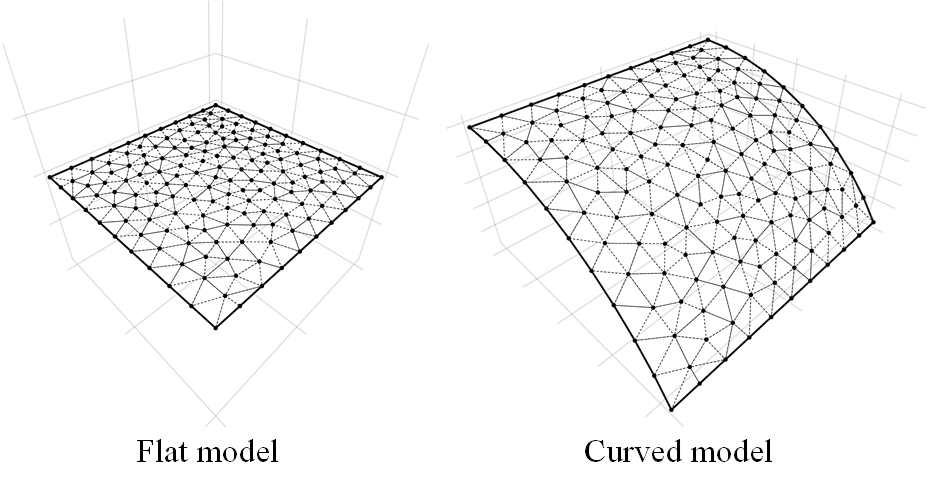
\includegraphics[width=\textwidth]{figures/ptmsh}
    \caption{Meshfree discretization for patch test}\label{ptf1}
\end{figure}

Table \ref{ptt1} lists the $L_2$- and $H_e$-Error results of patch test with flat model, where the RKGSI scheme with variational consistent essential boundary enforcement, i.e. RKGSI-Nitsche and RKGSI-HW, can pass the linear and quadratic patch test. \DIFaddbegin \DIFadd{In contrast, the RKGSI-Penalty cannot pass the patch test since the Penalty method is unable to ensure the variational consistency. }\DIFaddend Due to the loss of variational consistency condition, even with Nitsche's method, Gauss meshfree formulations show noticeable errors. Table \ref{ptt2} shows the results for curved model, which indicated that all the considered methods cannot pass the patch test. This is mainly because the proposed smoothed gradient of Eqs. (\ref{approxse1}) and (\ref{approxse2}) could not exactly reproduce the non-polynomial membrane and bending stress. However, the RKGSI-HW and RKGSI-Nitsche methods also provide better accuracy compared to others due to the fulfillment of first second-order variational consistency. \DIFaddbegin \DIFadd{And, even only with local variational consistency, the RKGSI-Penalty obtained a better result than traditional Gauss scheme. }\DIFaddend Meanwhile, the bending moment contours of $M^{12}$ are listed in Fig. \ref{ptf2}, which further verify that the proposed method provided a satisfactory result compared to exact solution. On the other hand, the \DIFaddbegin \DIFadd{RKGSI-Penalty and the }\DIFaddend conventional Gauss meshree formulations showed errors.

\begin{table}[!ht]
\centering
\caption{Results of patch test for flat model.}\label{ptt1}
\begin{tabular}{lcccc}
\toprule
 & \multicolumn{2}{c}{Linear patch test} & \multicolumn{2}{c}{Quadratic patch test} \\ \cline{2-5}
 & $L_2$-Error & $H_e$-Error & $L_2$-Error & $H_e$-Error \\
    \midrule
    GI-Penalty & $4.45E-4$ & $1.35E-2$ & $2.01E-3$ & $1.63E-2$ \\
    GI-Nitsche & $4.51E-4$ & $1.42E-2$ & $1.22E-3$ & $1.68E-2$ \\
    RKGSI-Penalty & $3.64E-9$ & $6.77E-8$ & $4.54E-9$ & $6.57E-8$ \\
    RKGSI-Nitsche & $3.31E-12$ & $1.34E-11$ & $5.98E-12$ & $1.21E-11$ \\
    RKGSI-HR & $6.67E-13$ & $1.50E-11$ & $1.07E-12$ & $1.26E-11$ \\
    \bottomrule
\end{tabular}
\end{table}

\begin{table}[!ht]
\centering
\caption{Results of patch test for cylindrical model.}\label{ptt2}
\begin{tabular}{lcccc}
\toprule
 & \multicolumn{2}{c}{Linear patch test} & \multicolumn{2}{c}{Quadratic patch test} \\ \cline{2-5}
 & $L_2$-Error & $H_e$-Error & $L_2$-Error & $H_e$-Error \\
    \midrule
    GI-Penalty & $3.79E-4$ & $1.30E-2$ & $1.74E-3$ & $1.37E-2$ \\
    GI-Nitsche & $4.04E-4$ & $1.42E-2$ & $1.15E-3$ & $1.49E-2$ \\
    RKGSI-Penalty & $1.47E-4$ & $5.39E-3$ & $2.26E-4$ & $2.09E-3$ \\
    RKGSI-Nitsche & $2.41E-6$ & $7.37E-5$ & $2.47E-6$ & $2.89E-5$ \\
    RKGSI-HR & $4.28E-6$ & $1.30E-4$ & $9.69E-6$ & $2.41E-4$ \\
    \bottomrule
\end{tabular}
\end{table}

\begin{figure}[!ht]
\centering
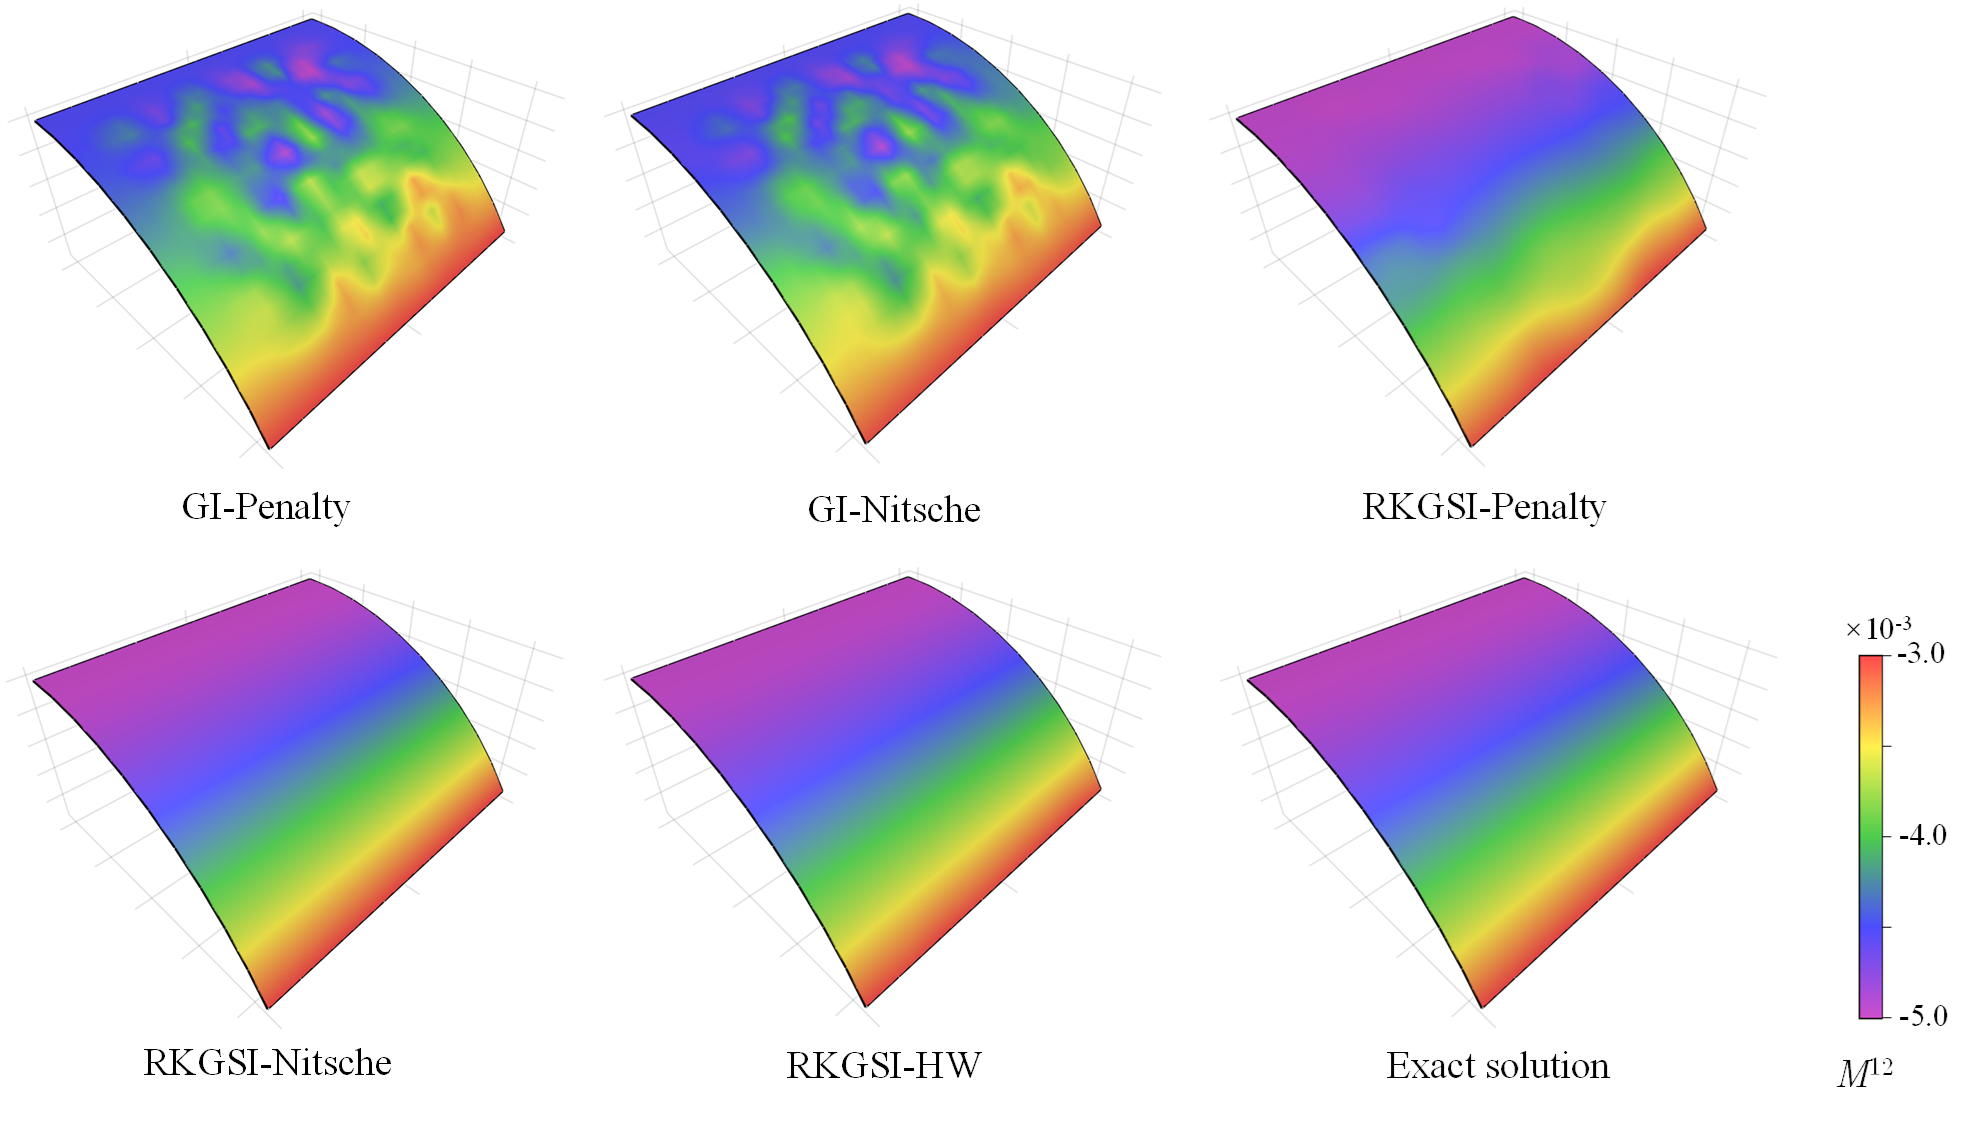
\includegraphics[width=\textwidth]{figures/ptc}
\caption{Contour plots of $M^{12}$ for curved shell patch test.}\label{ptf2}
\end{figure}

\subsection{Scordelis-Lo roof}
This example considers the classical Scordelis-Lo roof problem, as depicted in Fig. \ref{slf1}. The cylindrical roof has dimensions $R=25$, $L=50$, $h=0.25$, Young's modulus $E=4.32\times 10^8$ and Poisson's ratio $\nu=0.0$. The entire roof is subjected to an uniform body force of $b_z = -90$, with the straight edges remainning free and the the curved edges are enforced by $v_x=v_z=0$.

Due to the symmetry, only a quadrant of the model is considered for meshfree analysis, which is discretized by the $11\times 16$, $13\times 20$, $17\times 24$ and $19\times28$ meshfree nodes, as listed in Fig. \ref{slf2}. The comparison of the displacement in $z-$direction at node $A$, $v_{A3}$, is used as the investigated quantity, with the reference value \DIFdelbegin \DIFdel{0.3024 given by \mbox{%DIFAUXCMD
\cite{macneal1985}}\hskip0pt%DIFAUXCMD
}\DIFdelend \DIFaddbegin \DIFadd{0.3006 given by \mbox{%DIFAUXCMD
\cite{kiendl2009}}\hskip0pt%DIFAUXCMD
}\DIFaddend . Firstly, Fig. \ref{slf3} presents a sensitivity study for the artificial parameters of \DIFdelbegin \DIFdel{$\alpha_v$'s , }\DIFdelend \DIFaddbegin \DIFadd{$\alpha_{vi}$'s and }\DIFaddend $\alpha_\theta$'s in the RKGSI meshfree formulations with Nitsche's method and penalty method\DIFdelbegin \DIFdel{. }\DIFdelend \DIFaddbegin \DIFadd{, where all of the parameters are scaled by the support size as, $\alpha_{v\alpha} = s^{-1}\bar \alpha_v$, $\alpha_{v3} = s^{-3} \bar \alpha_v$ and $\alpha_\theta = s^{-1}\bar \alpha_\theta$. For a better comparison, the result of proposed RKGSI-HW is also listed in this figure. }\DIFaddend The results of Fig. \ref{slf3} revealed, Nitsche's method observed less artificial sensitivity. However, both the methods cannot trivially determine the optimal values of the artificial parameters. The optimal artificial parameters from Fig. \ref{slf3} are adopted for the convergence study in Fig. \ref{slf4}. The convergence result showed that the RKGSI get satisfactory results while the traditional Gauss methods demonstrated noticeable errors.

\begin{figure}[!ht]
\centering
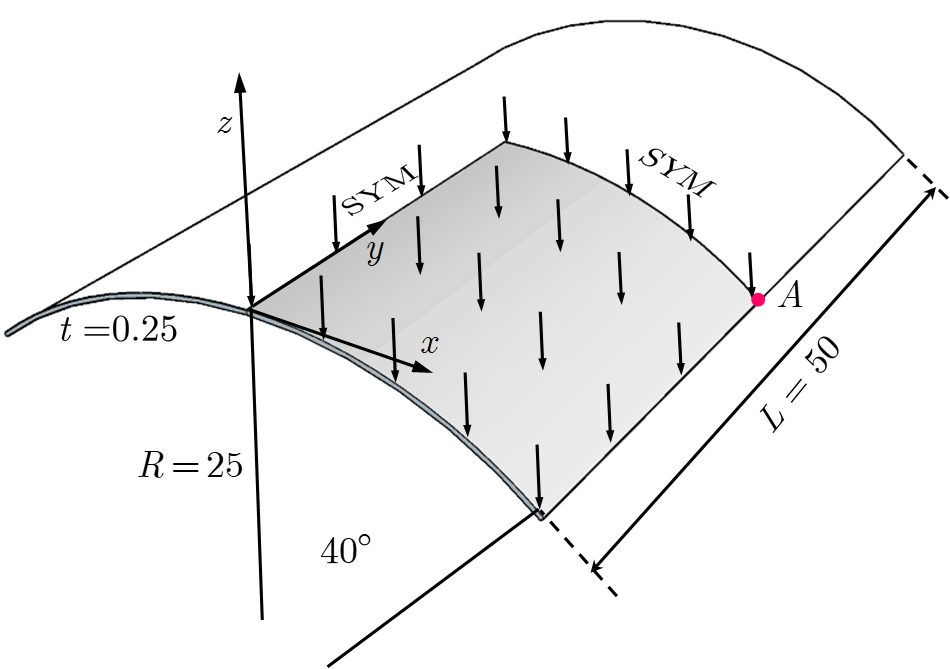
\includegraphics[width=0.7\textwidth]{figures/slm}
\caption{Description of Scordelis-Lo roof problem.}\label{slf1}
\end{figure}
\begin{figure}[!ht]
\centering
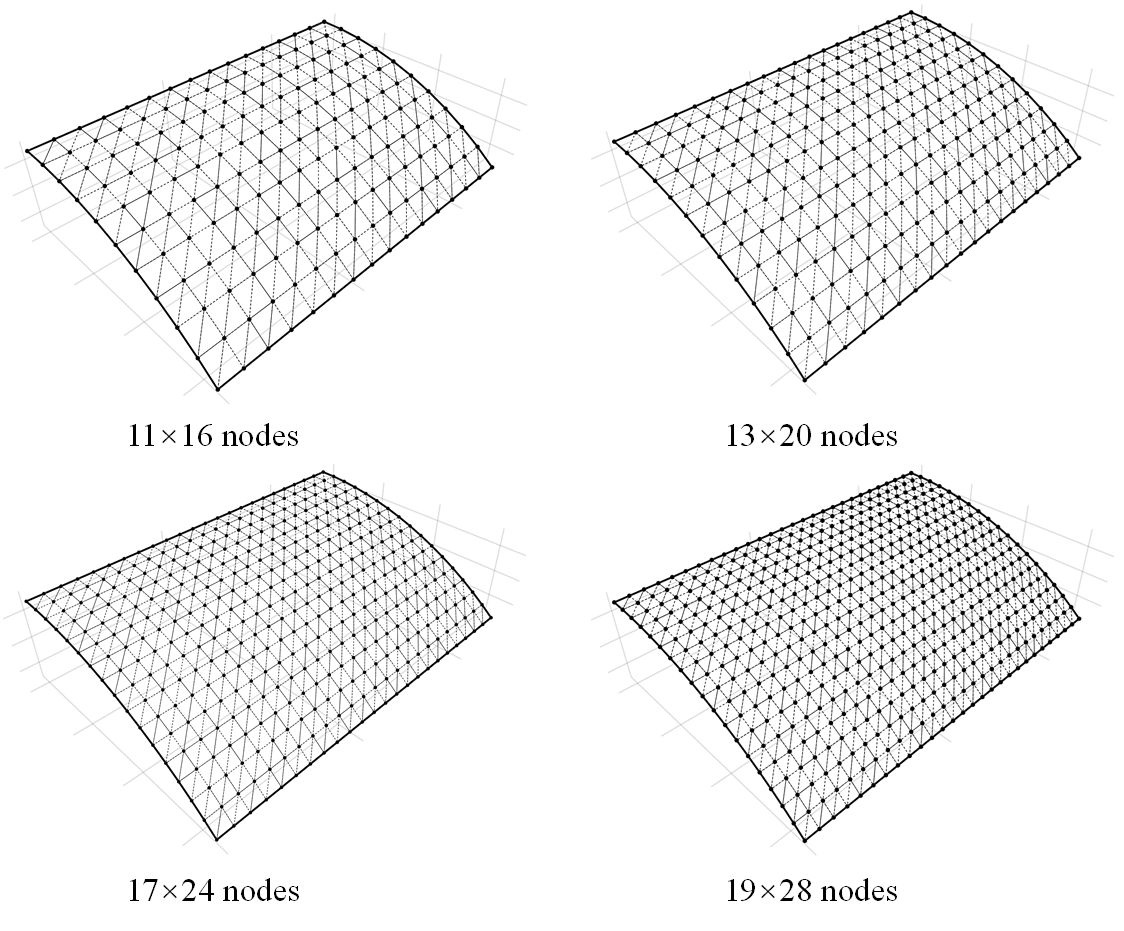
\includegraphics[width=\textwidth]{figures/slmsh}
\caption{Meshfree discretizations for Scordelis-Lo roof problem.}\label{slf2}
\end{figure}
\begin{figure}[!ht]
\centering
\DIFdelbeginFL %DIFDELCMD < 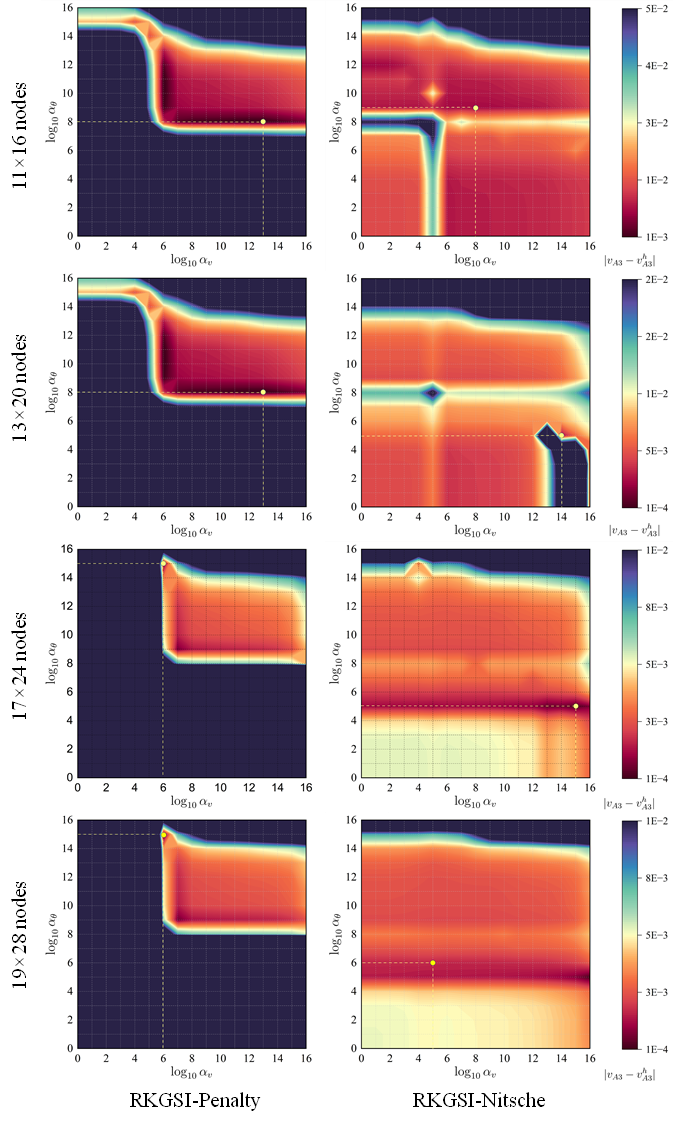
\includegraphics[width=\textwidth]{figures/sla}
%DIFDELCMD < %%%
\DIFdelendFL \DIFaddbeginFL 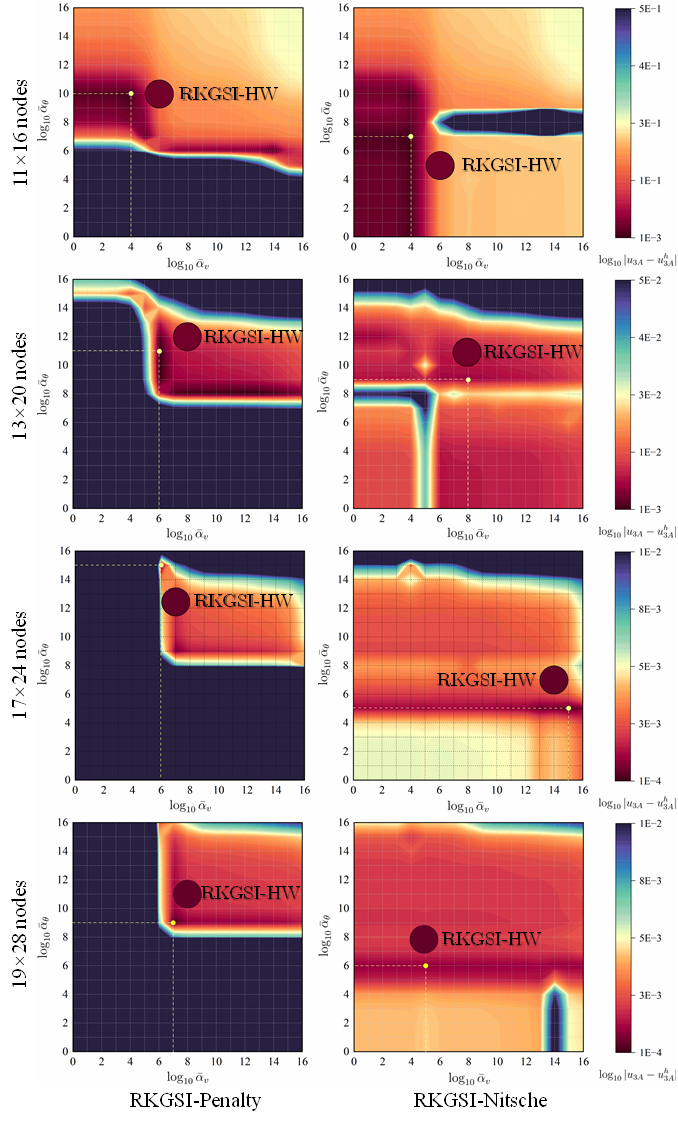
\includegraphics[width=\textwidth]{figures/sla_r1}
\DIFaddendFL \caption{Sensitivity comparison of $\alpha_v$ and $\alpha_\theta$ for Scordelis-Lo problem.}\label{slf3}
\end{figure}
\begin{figure}[!ht]
\centering
\DIFdelbeginFL %DIFDELCMD < 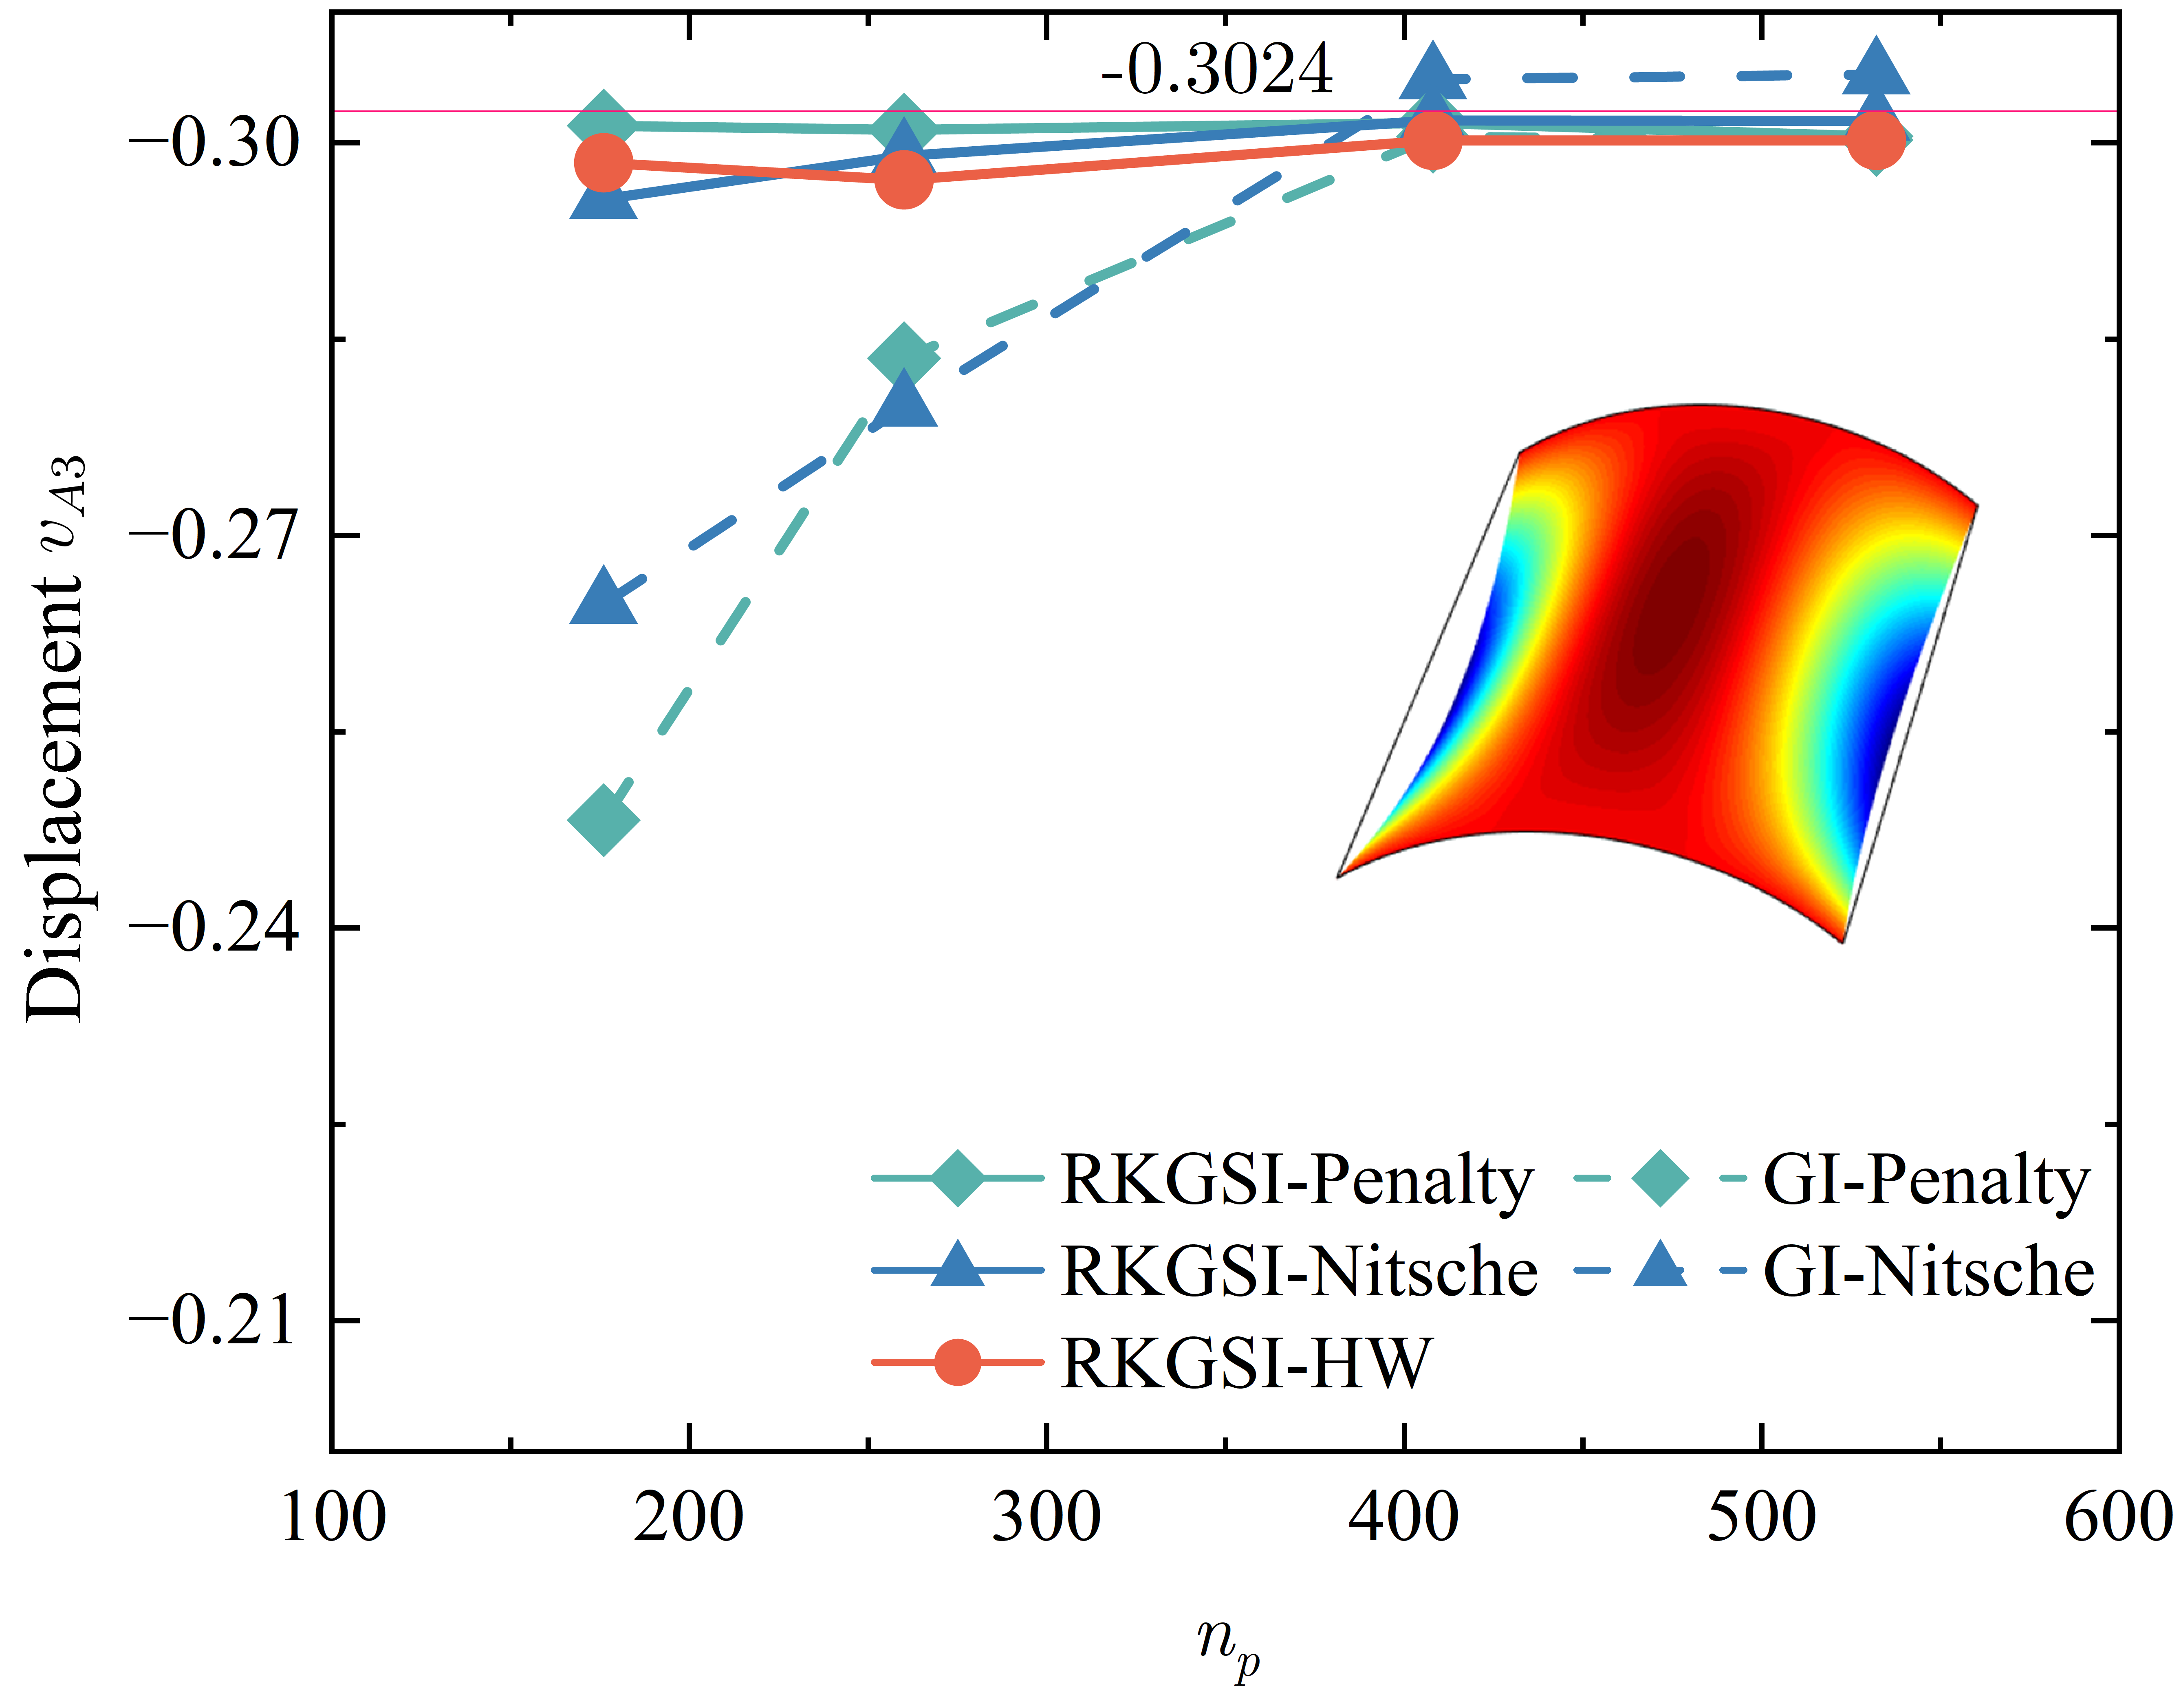
\includegraphics[width=\textwidth]{figures/sld}
%DIFDELCMD < %%%
\DIFdelendFL \DIFaddbeginFL 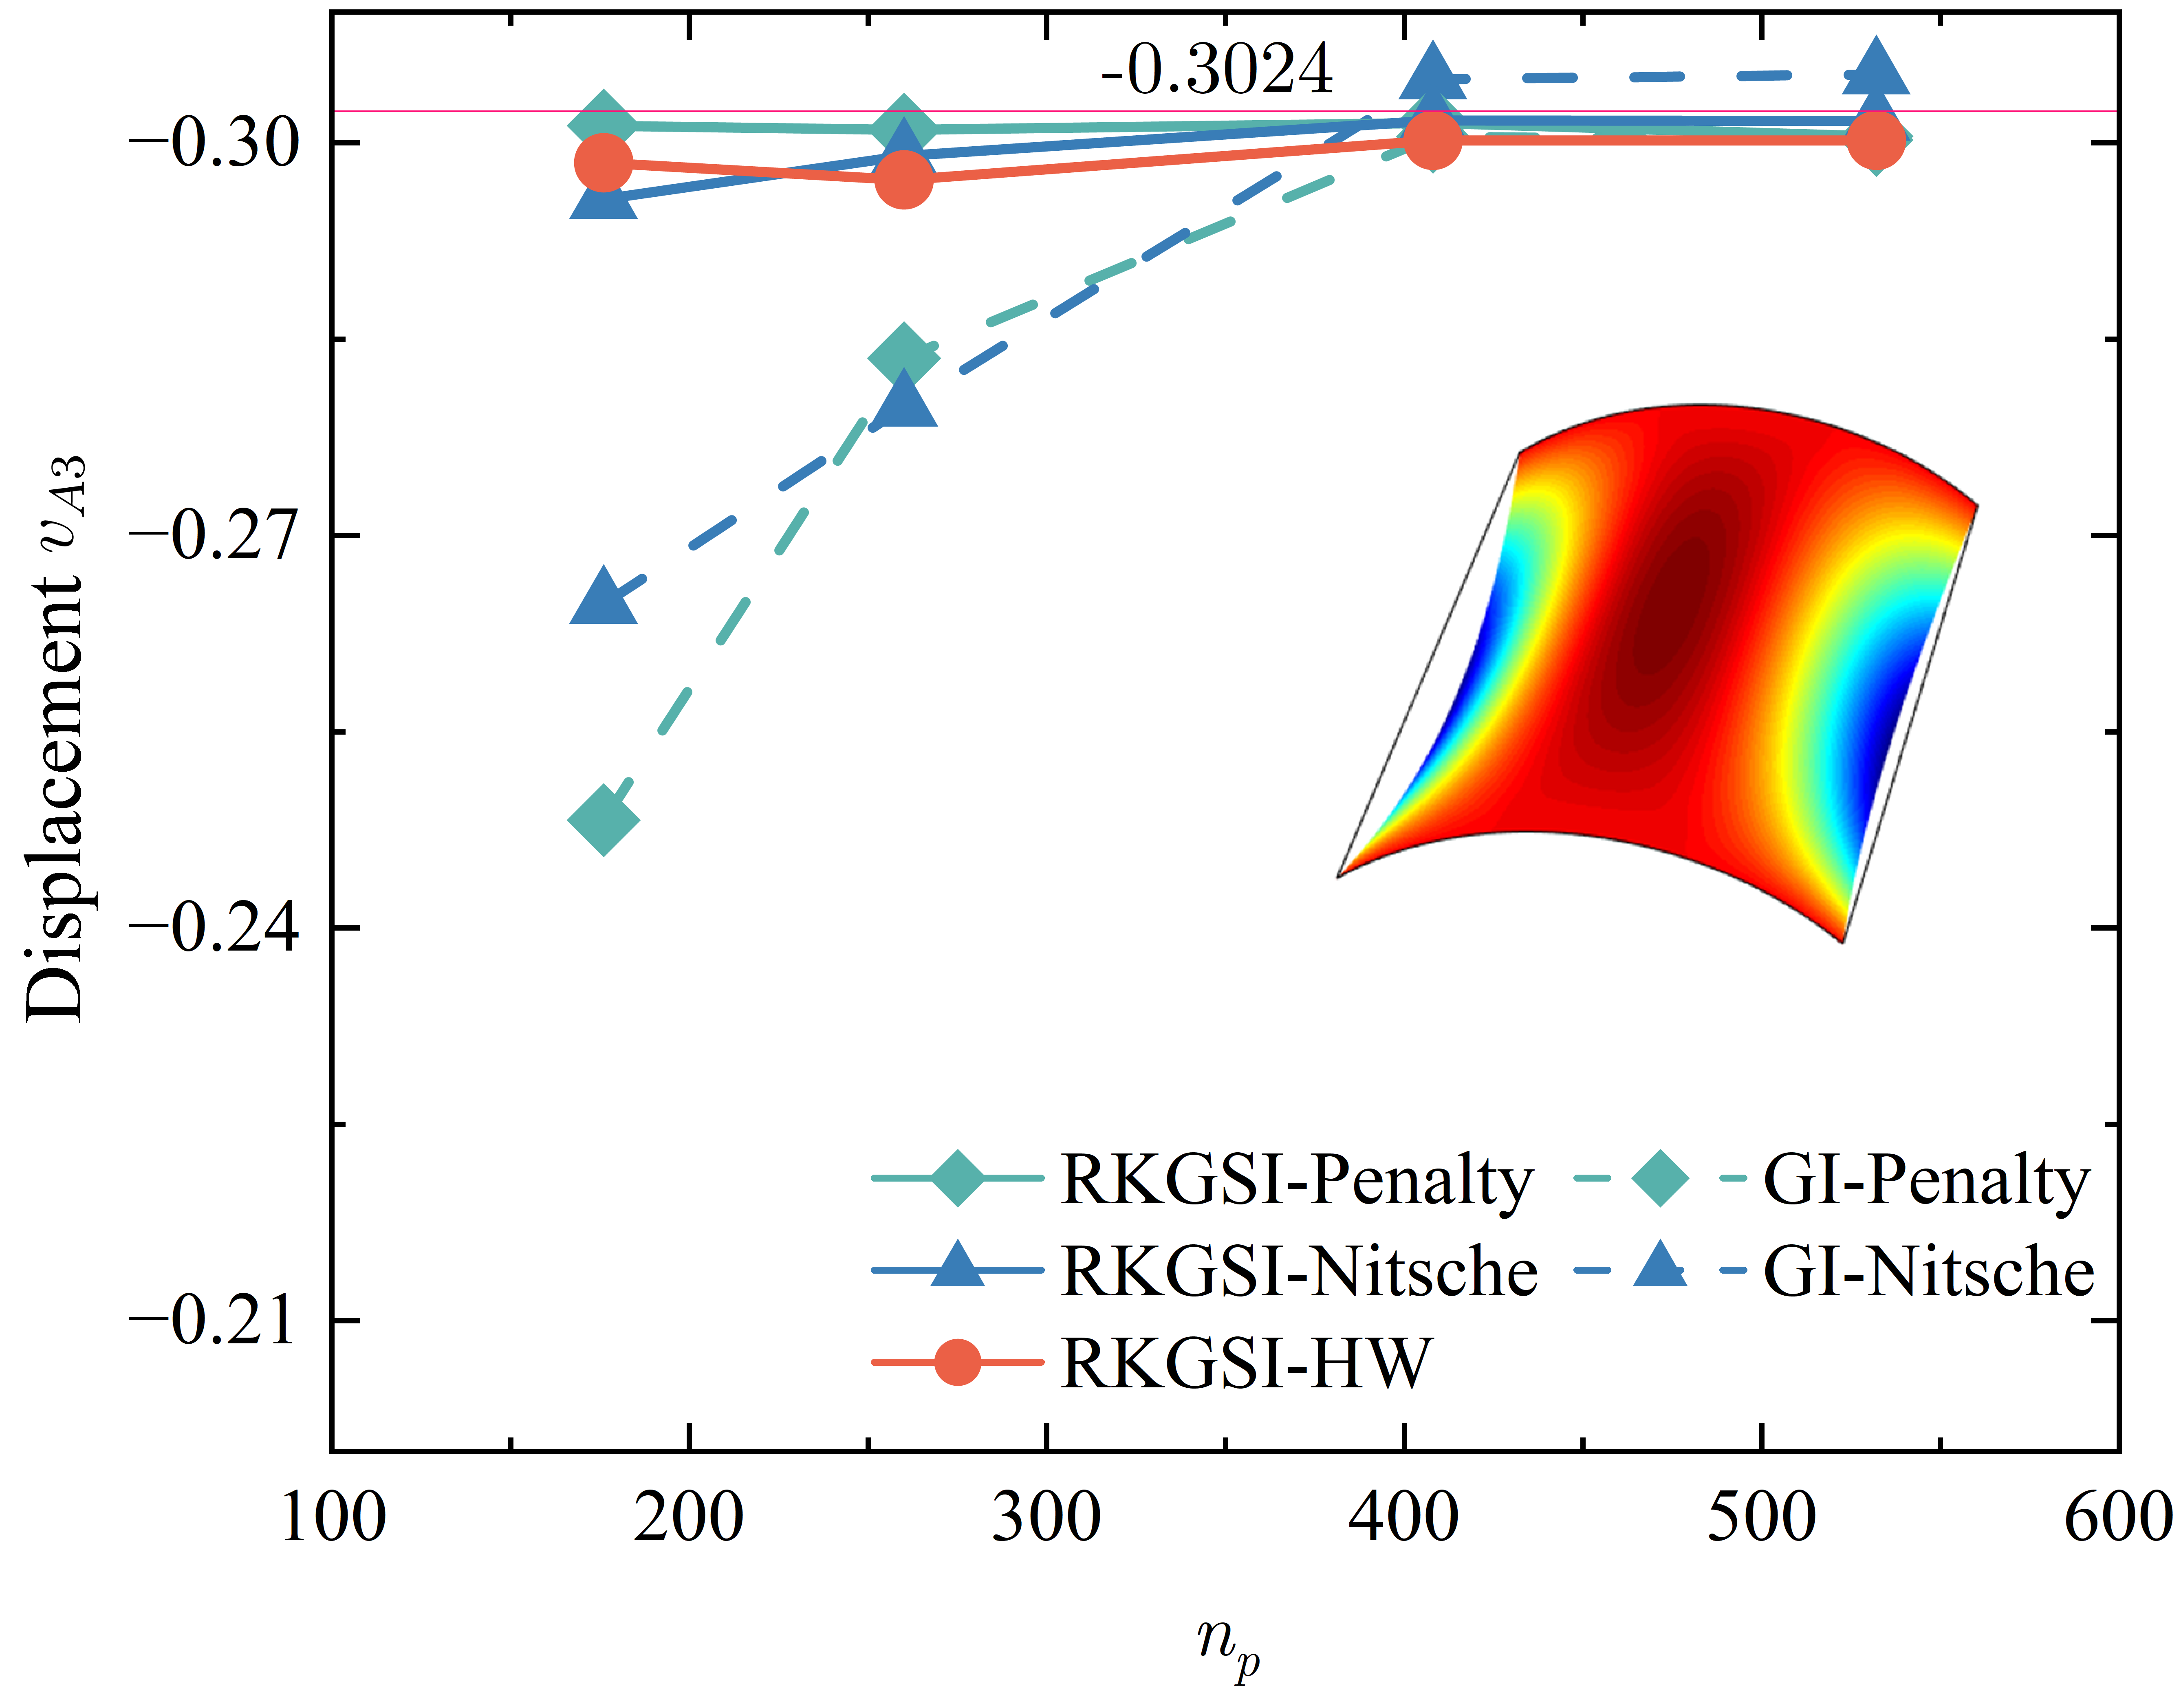
\includegraphics[width=\textwidth]{figures/sld_r1}
\DIFaddendFL \caption{Displacement convergence for Scordelis-Lo roof problem.}\label{slf4}
\end{figure}

\subsection{Pinched Hemispherical shell}
Consider the hemispherical shell shown in Fig. \ref{phf1}, which is loaded at four points $P=\pm 2$ at $90^\circ$ interval at its bottom. The hemispherical shell has an radius $R=10$, thickness $h=0.04$, Young's modulus $E=6.825\times10^7$ and Poisson's ratio $\nu = 0.3$.

Due to symmetry, only quadrant model, where the \DIFdelbegin \DIFdel{$8\times8$, }\DIFdelend $16\times16$, $24\times24$\DIFdelbegin \DIFdel{and }\DIFdelend \DIFaddbegin \DIFadd{, }\DIFaddend $32\times32$ \DIFaddbegin \DIFadd{and $40\times40$ }\DIFaddend meshfree nodes have been discretized \DIFaddbegin \DIFadd{as shown in Fig. (\ref{phfm})}\DIFaddend , was considered. The quantity under investigation for convergence is the displacement at $x-$direction on point $A$, $v_{A1}$.
Fig. \ref{phf2} displays the corresponding convergence results, indicating the RKGSI scheme performed significantly better compared to the GI meshfree formulation. Meanwhile, the efficiency comparison for this problem is also shown in Fig. \ref{phf3}, in which the CPU time for assembly and calculation of shape functions are considered. Fig. \ref{phf3}(a) indicates that the RKGSI scheme observed high efficiency in assembly. This is due to the variational inconsistent Gauss meshfree formulation which require more Gaussian points to get satisfactory results. Fig. \ref{phf3}(b) lists the CPU time spent on enforcing essential boundary conditions for the penalty method, Nitsche's method and proposed HW method. The results highlighted that the proposed HW method consumed comparable CPU time in assembly compared to Nitsche's method. However, less time was spent to calculate the shape functions. Since both the HW method and penalty method were developed considering the shape functions first order derivatives. For this reason, both the methods shared an almost identical time in computing the shape functions.
\begin{figure}[!ht]
\centering
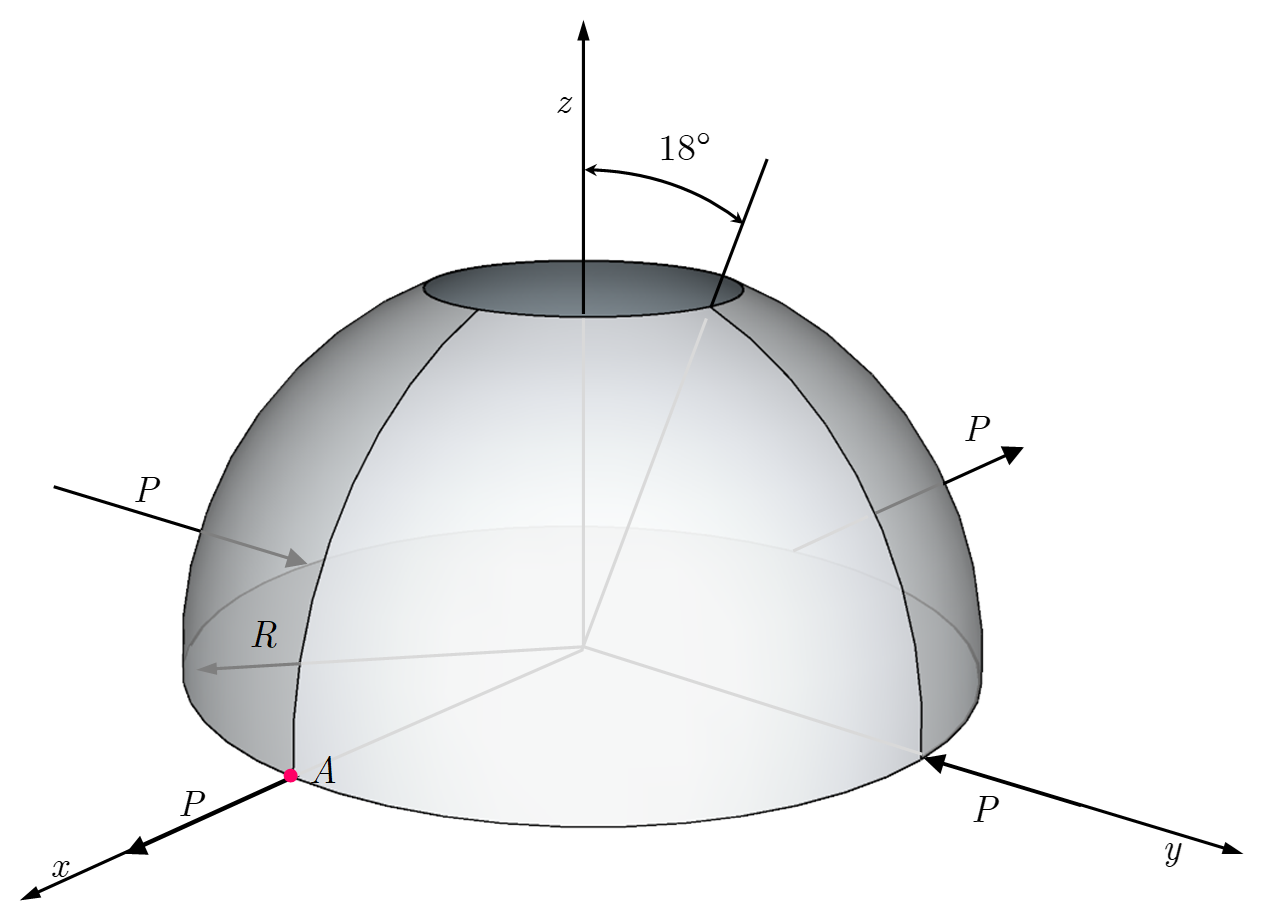
\includegraphics[width=0.8\textwidth]{figures/pfm}
\caption{Description of pinched hemispherical shell problem.}\label{phf1}
\end{figure}
\begin{figure}[!ht]
\centering
\DIFdelbeginFL %DIFDELCMD < 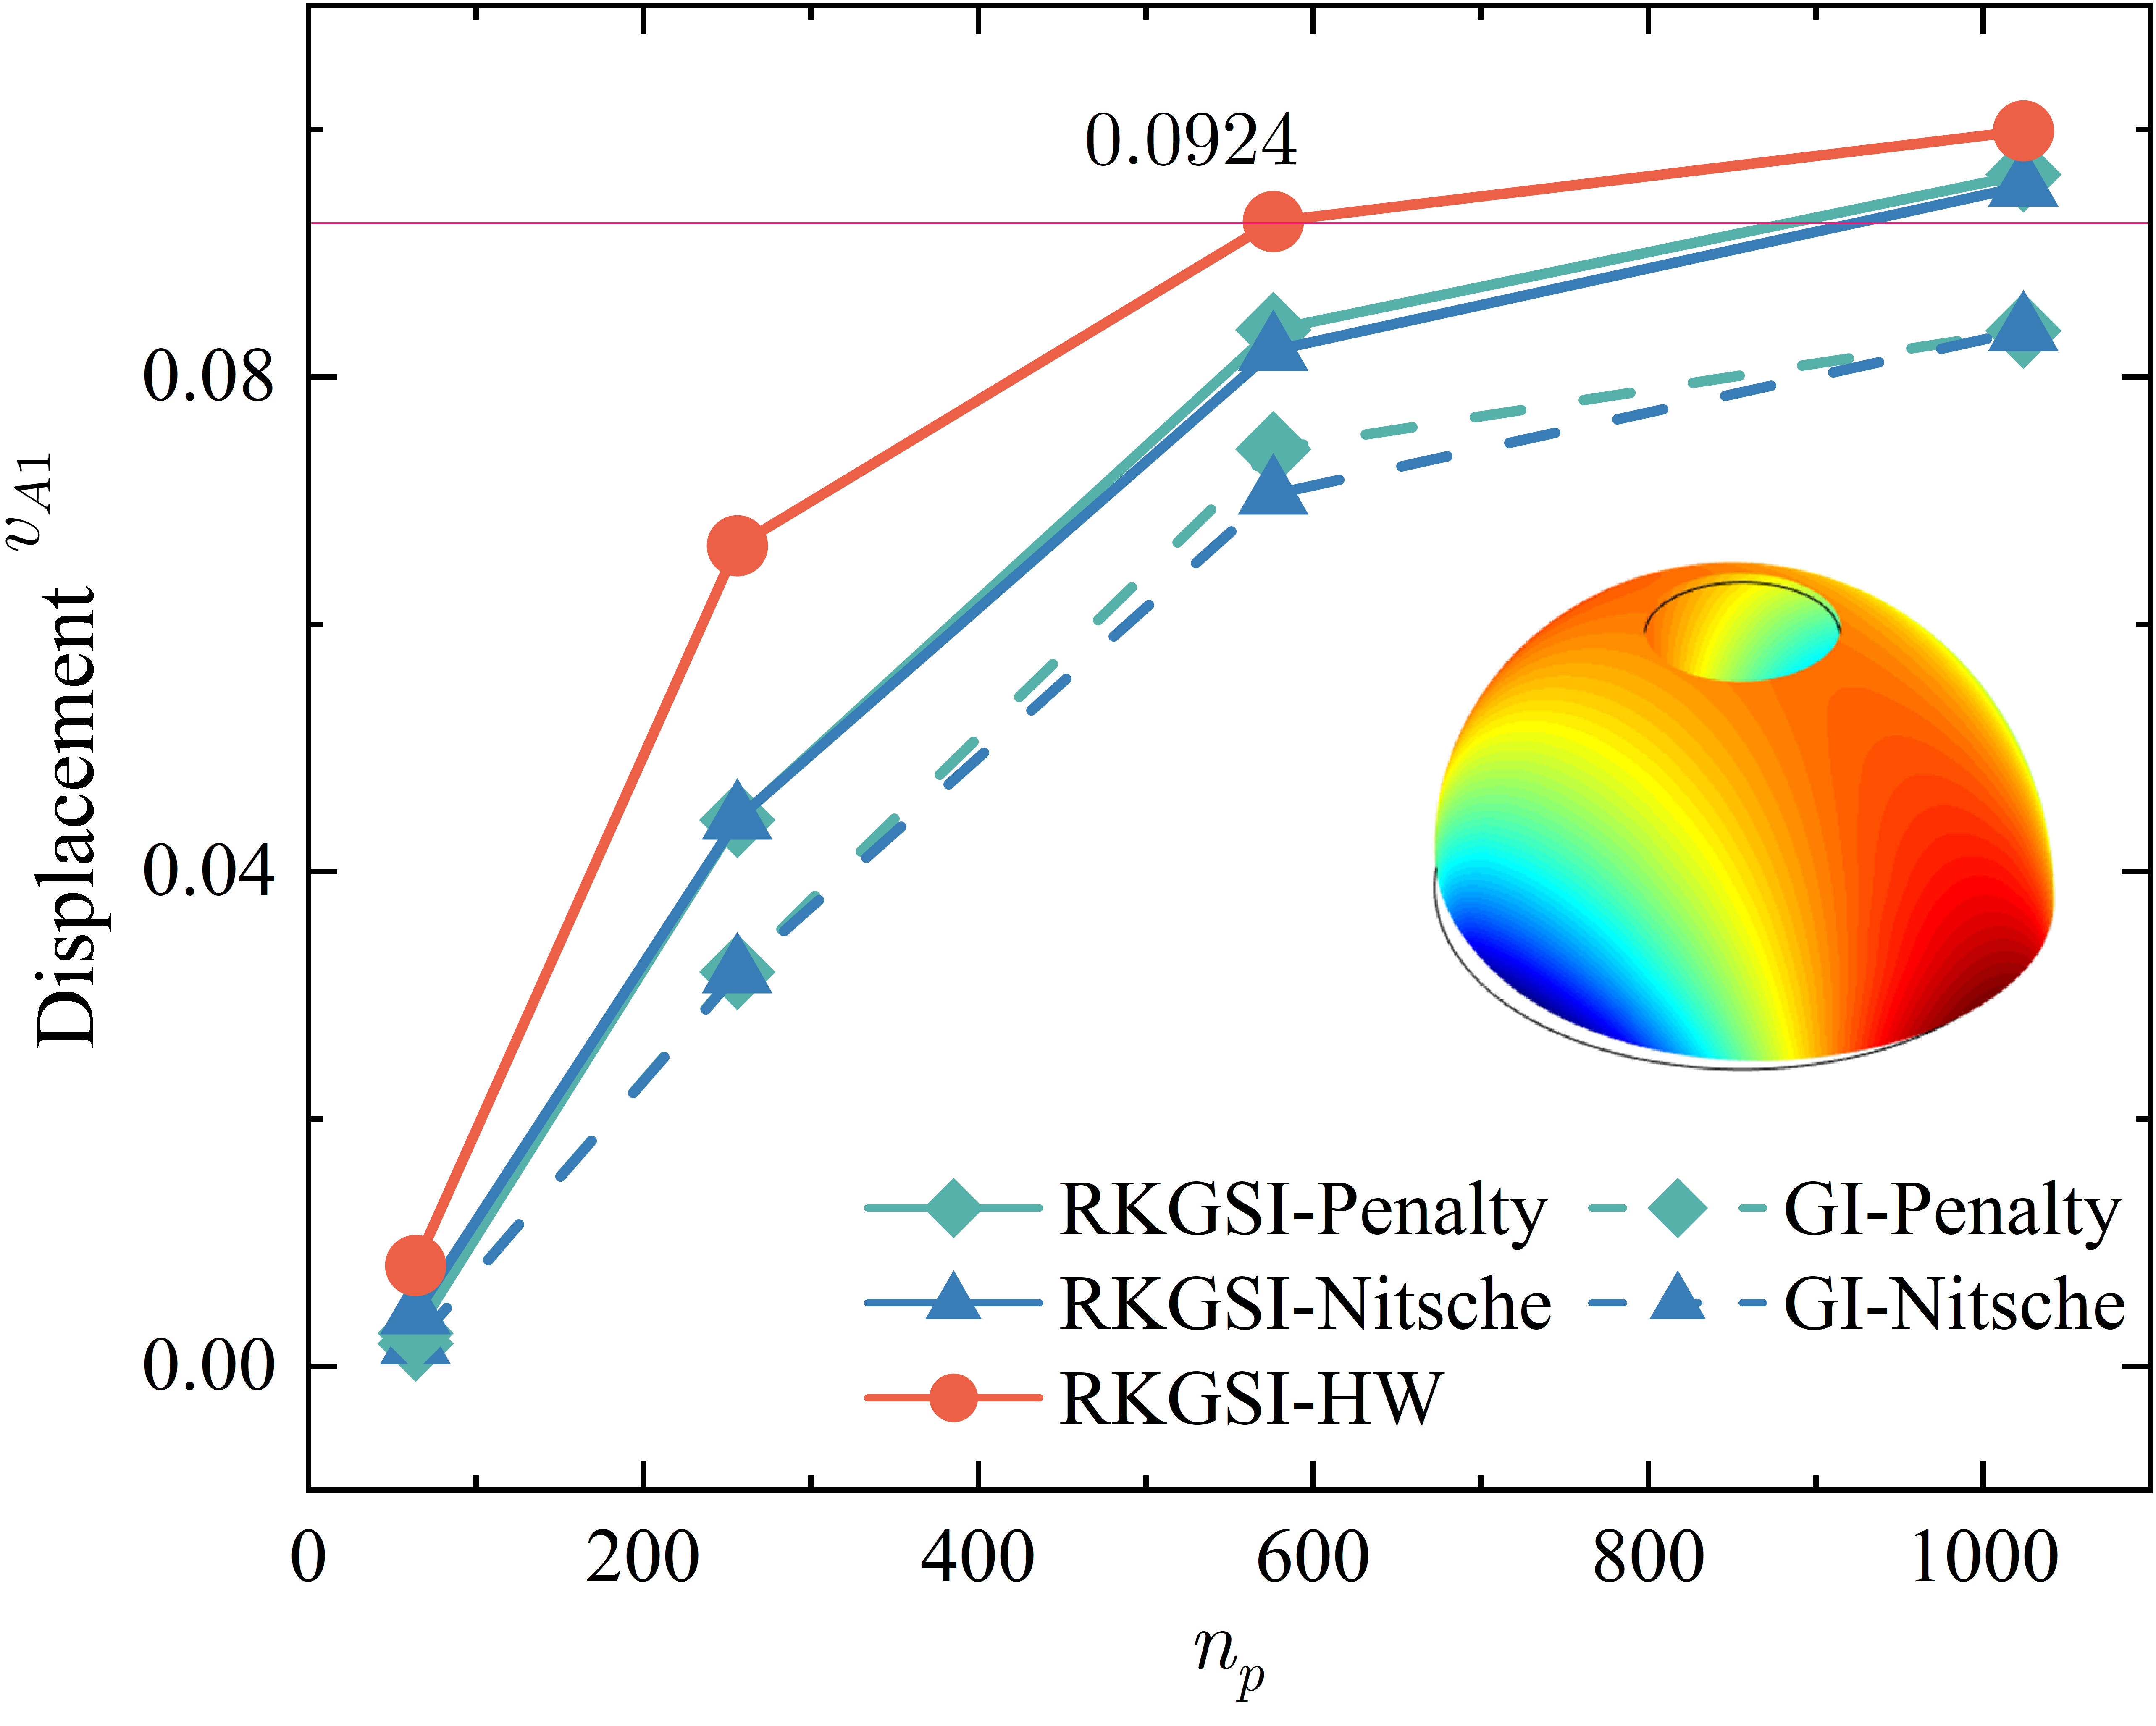
\includegraphics[width=\textwidth]{figures/pfd}
%DIFDELCMD < %%%
\DIFdelendFL \DIFaddbeginFL 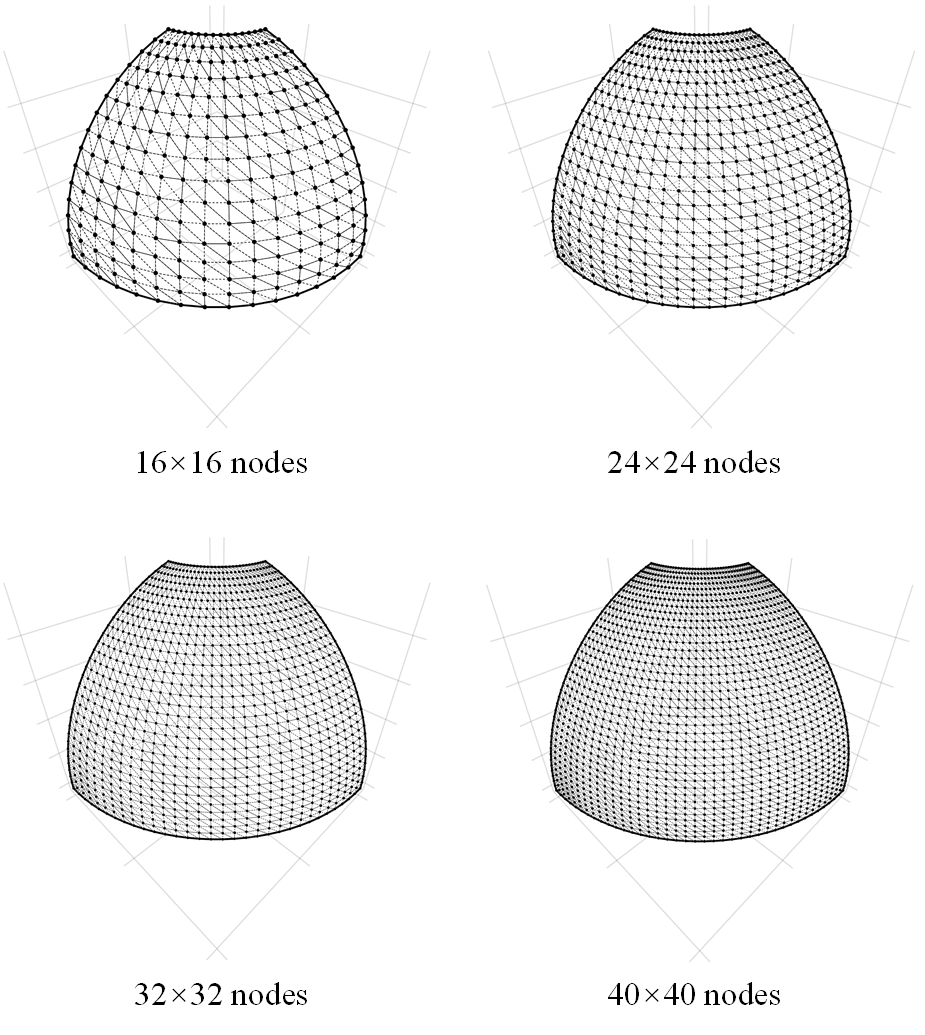
\includegraphics[width=\textwidth]{figures/pfmsh_r1}
\caption{\DIFaddFL{Meshfree discretizations for pinched hemispherical shell problem.}}\label{phfm}
\end{figure}
\begin{figure}[!ht]
\centering
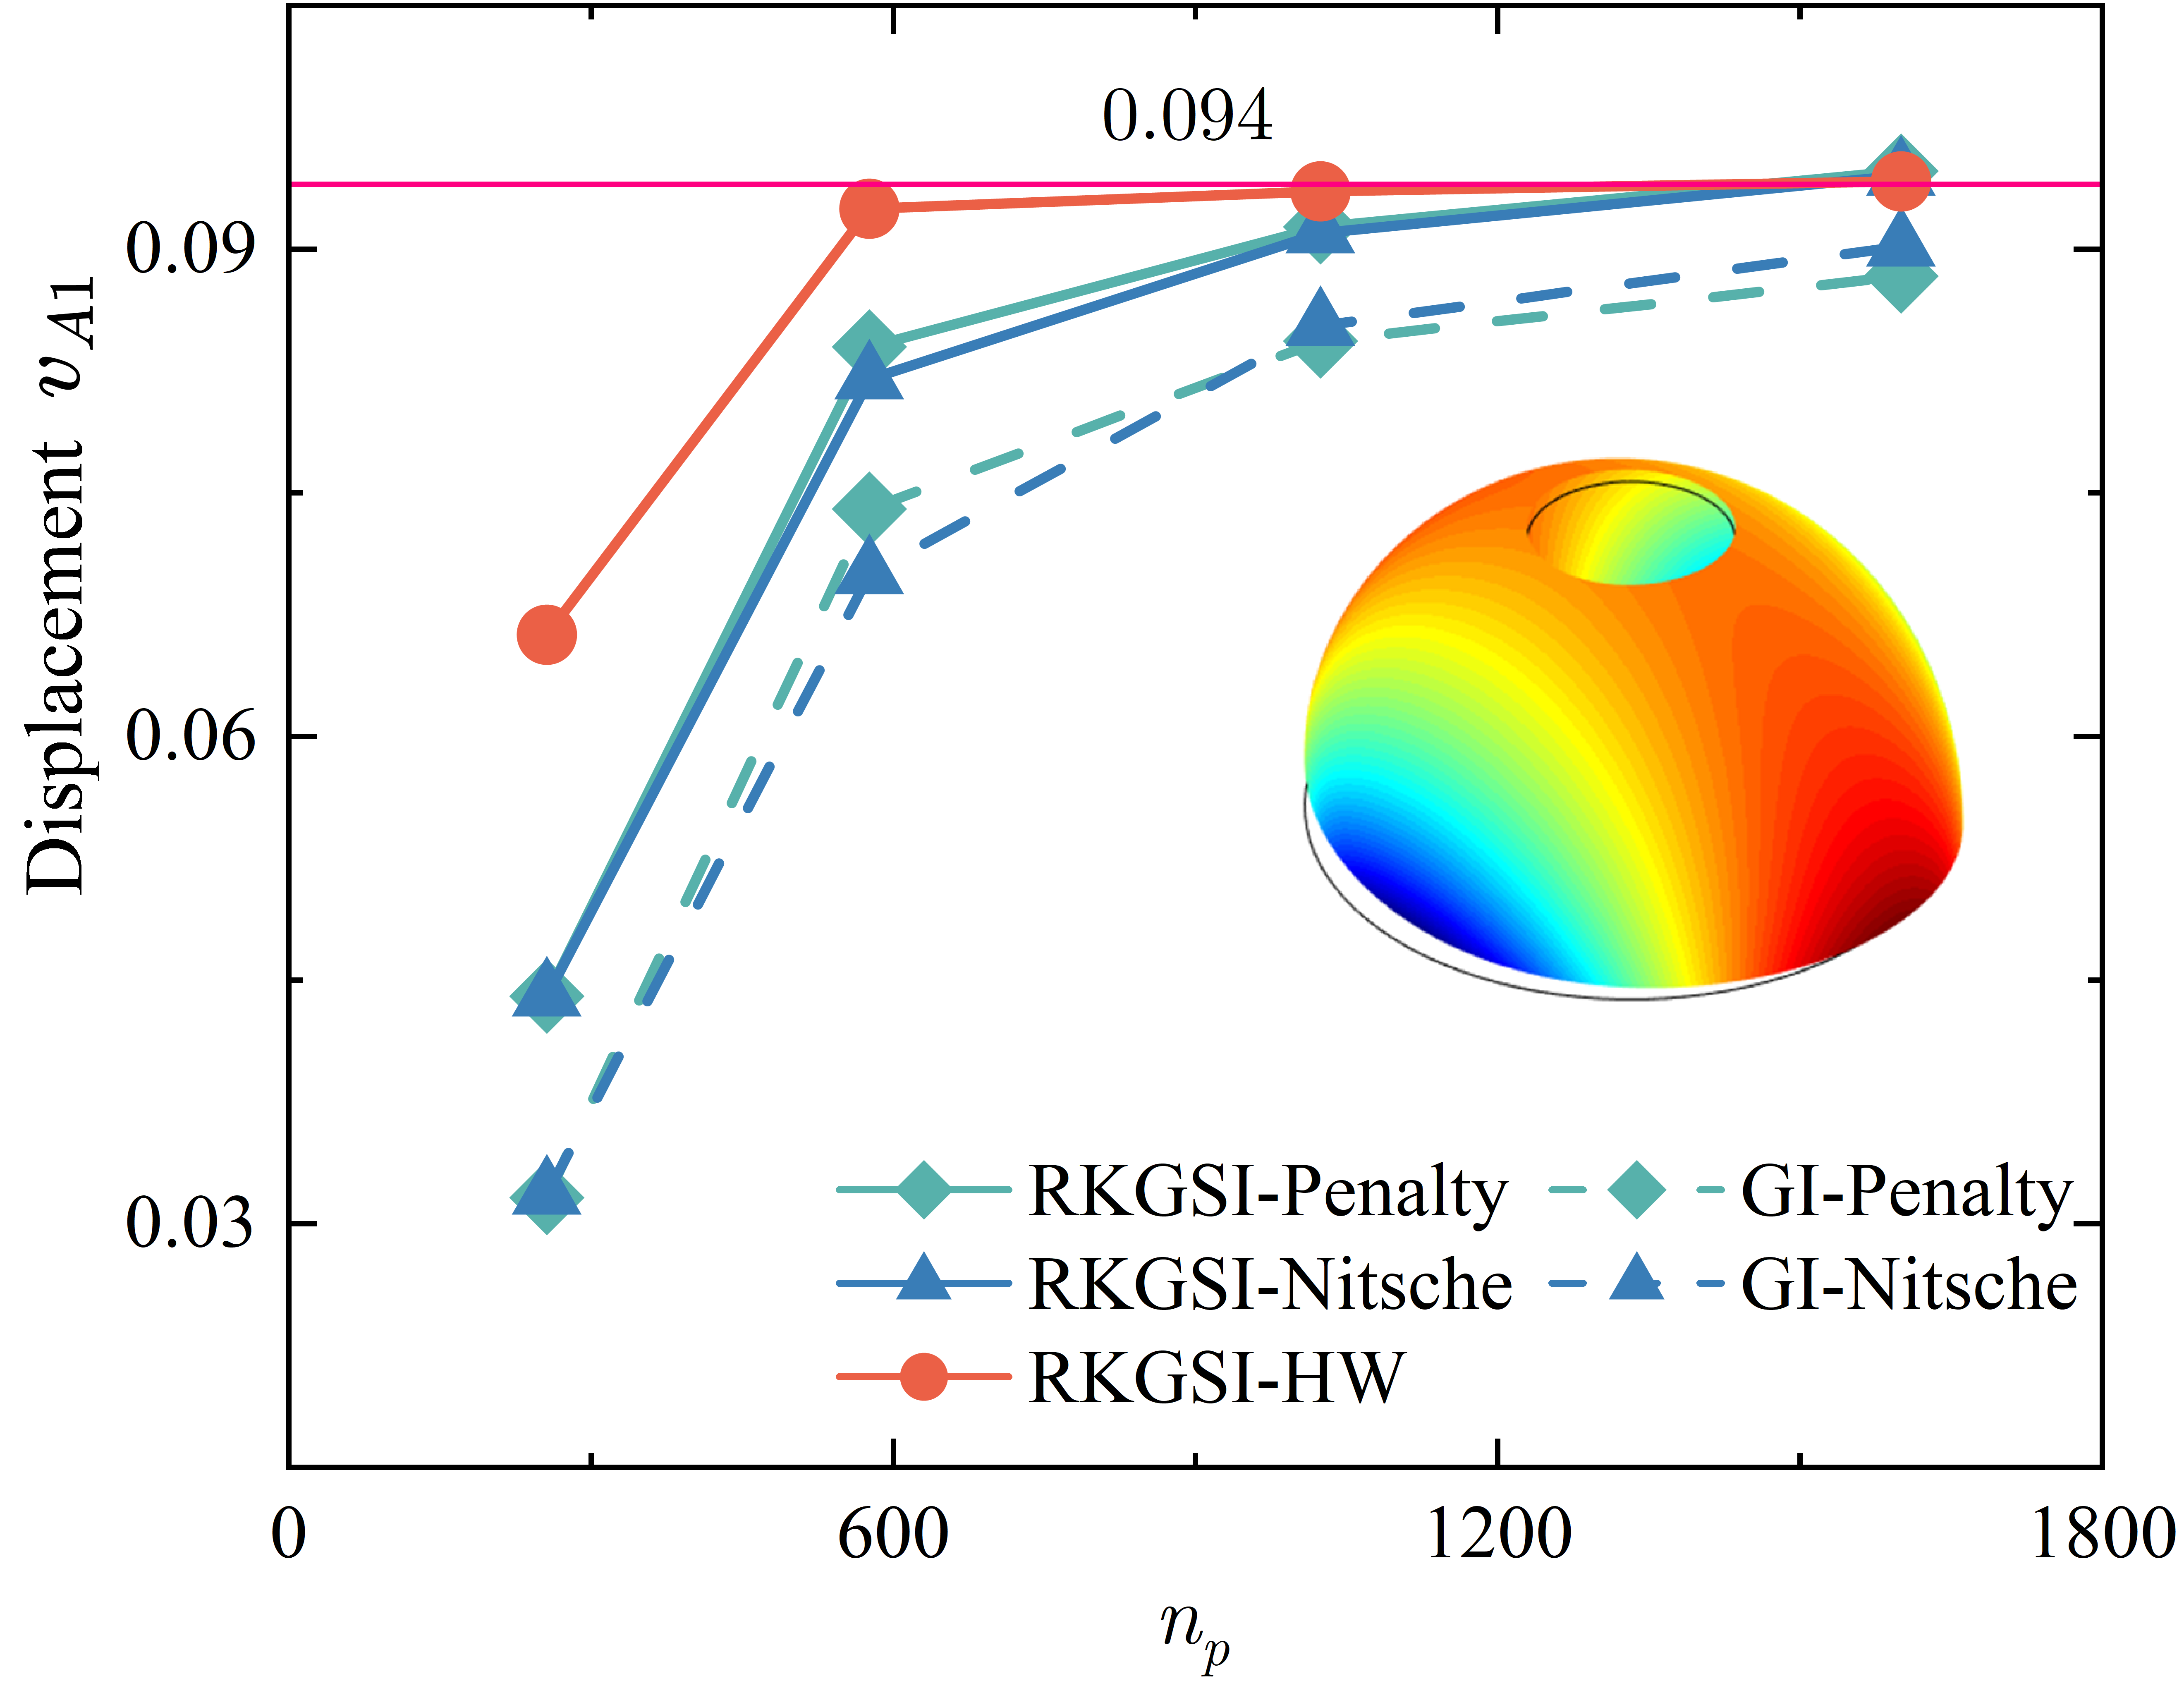
\includegraphics[width=\textwidth]{figures/pfd_r1}
\DIFaddendFL \caption{Displacement convergence for pinched hemispherical shell problem.}\label{phf2}
\end{figure}
\begin{figure}[!ht]
\centering
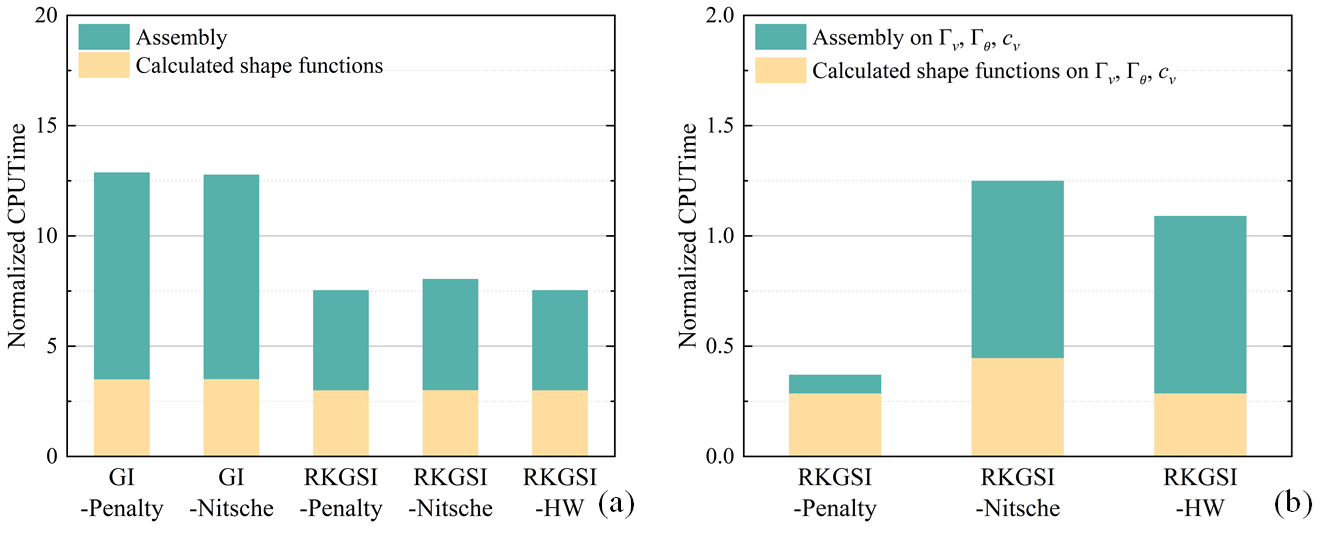
\includegraphics[width=\textwidth]{figures/efficient}
\caption{efficiency comparison for pinched hemispherical shell problem: (a) Whole domain; (b) Essential boundaries}\label{phf3}
\end{figure}



\section{Conclusion}\label{conclusion}
In this study, an efficient and quasi-consistent meshfree thin shell formulation was presented to naturally enforce the essential boundary conditions.  Mixed formulation with the Hu-Washizu principle weak form is adopted, where the traditional meshfree shape functions discretized the displacement, and the strains and stresses were expressed by the reproducing kernel smoothed gradients and the covariant smoothed gradients, respectively. The smoothed gradient naturally embedded the first second-order integration constraints and has a quasi variational consistency for the curved models in each integration cell. Owing to the Hu-Washizu variational principle, the essential boundary condition enforcement has a similar form with the conventional Nitsche’s method; both have consistent and stabilized terms. The costly high order derivatives in the Nitsche’s consistent term have been replaced by the smoothed gradients, which improved the computational speed due to the reproducing kernel gradient smoothing framework. Furthermore, the stabilized term naturally existed in the Hu-Washizu weak form, and the artificial parameter needed in Nitsche’s stabilized term has vanished, which can automatically maintain the coercivity for the stiffness matrix. \DIFaddbegin \DIFadd{Based on general reproducing kernel gradient smoothing framework, the proposed methodology can be trivially extended to high order basis meshfree formulation. }\DIFaddend The numerical results demonstrated that the proposed Hu-Washizu quasi-consistent meshfree thin shell formulation showed excellent accuracy, efficiency, and stability.


\DIFaddend \section*{Acknowledgment}
The support of this work by the National Natural Science Foundation of China (12102138, 52350410467) and the Natural Science Foundation of Fujian Province of China (2023J01108, 2022J05056) is gratefully acknowledged.
\appendix
\section{Covariant derivatives}\label{appderivative}
This Appendix lists the covariant derivatives needed for the development of the proposed method. For an arbitrary first order tensor $\boldsymbol v$ presented by in-plane covariant or contravariant bases as: 
\begin{equation}
\boldsymbol v = v_{\alpha}\boldsymbol a^\alpha + v_{3} \boldsymbol a_3 = v^{\alpha}\boldsymbol a_\alpha + v^3 \boldsymbol a_3
\end{equation}
the partial derivatives of tensor $\boldsymbol v$ with respect to coordinate $\xi^\alpha$, $\boldsymbol v_{,\alpha}$, can be evaluated by:
\begin{equation}
\begin{split}
\boldsymbol v_{,\alpha} &= 
v_{\beta,\alpha} \boldsymbol a^\beta + v_{\beta}\boldsymbol a^\beta_{,\alpha} + v_{3,\alpha}\boldsymbol a_3 + v_3 \boldsymbol a_{3,\alpha} \\
&= v_{\beta,\alpha} \boldsymbol a^\beta - \Gamma^\beta_{\alpha\gamma}v_\beta \boldsymbol a^\gamma + v_{3,\alpha} \boldsymbol a_3 - v_3 b_{\alpha\beta} \boldsymbol a^\beta \\
&= v_{\beta,\alpha} \boldsymbol a^\beta - \Gamma^\gamma_{\alpha\beta}v_\gamma \boldsymbol a^\beta + v_{3,\alpha} \boldsymbol a_3 - v_3 b_{\alpha\beta} \boldsymbol a^\beta \\
&= v_{\beta}\vert_\alpha \boldsymbol a^\beta + v_{3,\alpha} \boldsymbol a_3 - v_3 b_{\alpha\beta} \boldsymbol a^\beta \\
\end{split}
\end{equation}
where $\Gamma^\gamma_{\alpha\beta} = \boldsymbol a_{\alpha,\beta}\cdot \boldsymbol a^\gamma$ denotes the Christoffel symbol of the second kind, $b_{\alpha\beta} = \boldsymbol a_{\alpha,\beta}\cdot\boldsymbol a_3=-\boldsymbol a_{\alpha}\cdot\boldsymbol a_{3,\beta}$ stands for the curvature tensor. $v_\alpha\vert_\beta$ can be regarded as the in-plane covariant derivative of the vector $v_\alpha$:
\begin{equation}
v_{\alpha}\vert_\beta = v_{\alpha,\beta} - \Gamma^\gamma_{\alpha\beta} v_\gamma
\end{equation}

Following the same path, the in-plane covariant derivative of $v^\alpha$ is given by:
\begin{equation}
v^\alpha\vert_\beta = v^\alpha_{,\beta} + \Gamma^\alpha_{\beta\gamma} v^\gamma
\end{equation}


\DIFdelbegin %DIFDELCMD < \section{Derivations for stiffness metrics and force vectors}\label{derivations}
This Appendix details the derivations of stiffness matrices and force vectors in Eqs. (\ref{de1})-(\ref{de3}), where the relationships of Eqs. (\ref{gn}), (\ref{gm}), (\ref{epsilon2}) and (\ref{kappa2}) are used herein. Firstly, the membrane strain terms are considered as follows:
\begin{equation}
\begin{split}
&\sum_{C=1}^{n_e}\int_{\Omega_C} \delta \tilde \varepsilon_{\alpha\beta}^h hC^{\alpha\beta\gamma\eta}\bar \varepsilon^h_{\gamma\eta} d\Omega \\
        =&\sum_{C=1}^{n_e}\sum_{I,J=1}^{n_p}\delta \boldsymbol d_I \cdot \underbrace{\int_{\Omega_C} \tilde{\boldsymbol \varepsilon}_{\alpha\beta I} hC^{\alpha\beta\gamma\eta} \boldsymbol a_\gamma \boldsymbol q^T d\Omega}_{\tilde{\boldsymbol g}^{\eta T}_I} \boldsymbol G^{-1} \bar{\boldsymbol g}_{\eta J} \cdot \boldsymbol d_J \\
        =&\sum_{C=1}^{n_e}\sum_{I,J=1}^{n_p}\delta \boldsymbol d_I \cdot \int_{\Gamma_C\cap\Gamma_v} \Psi_J \underbrace{\boldsymbol q^T \boldsymbol G^{-1}\tilde{\boldsymbol g}^\alpha_I
        n_\alpha}_{\tilde{\boldsymbol T}_{NI}} d\Gamma
       \cdot \boldsymbol d_J \\
        =&\sum_{I,J=1}^{n_p}\delta \boldsymbol d_I \cdot \int_{\Gamma_v} \tilde{\boldsymbol T}_{NI}\Psi_J d\Gamma
       \cdot \boldsymbol d_J \\
\end{split}
\end{equation}
with
\begin{equation}
        \tilde{\boldsymbol g}^\alpha_I = \boldsymbol q \boldsymbol a_\beta hC^{\alpha\beta\gamma\eta} \tilde{\boldsymbol \varepsilon}_{\alpha\beta I}
\end{equation}
\begin{equation}
        \tilde{\boldsymbol T}_{NI} = \boldsymbol q^T \boldsymbol G^{-1} \tilde{\boldsymbol g}_I^\alpha n_\alpha
\end{equation}

Following this path, the bending strain terms can be reorganized by:
\begin{equation}
\begin{split}
&\sum_{C=1}^{n_e}\int_{\Omega_C} \delta \tilde \kappa_{\alpha\beta}^h \frac{h^3}{12}C^{\alpha\beta\gamma\eta}\bar \kappa^h_{\gamma\eta} d\Omega \\
        =&\sum_{C=1}^{n_e}\sum_{I,J=1}^{n_p}\delta \boldsymbol d_I \cdot \underbrace{\int_{\Omega_C} \tilde{\boldsymbol \kappa}_{\alpha\beta I} \frac{h^3}{12}C^{\alpha\beta\gamma\eta} \boldsymbol a_3 \boldsymbol q^T d\Omega}_{\tilde{\boldsymbol g}^{\gamma\eta T}_I} \boldsymbol G^{-1} \bar{\boldsymbol g}_{\gamma\eta J} \cdot \boldsymbol d_J \\
        =&\sum_{C=1}^{n_e}\sum_{I,J=1}^{n_p}\delta \boldsymbol d_I \cdot \left (
        \begin{split}
                &\int_{\Gamma_C\cap\Gamma_\theta} \underbrace{\boldsymbol q^T \boldsymbol G^{-1}\tilde{\boldsymbol g}^{\alpha\beta}_I n_\alpha n_\beta}_{\tilde{\boldsymbol M}_{\boldsymbol{nn} I}} n^\gamma\Psi_{J,\gamma} d\Gamma \\
                - &\int_{\Gamma_C\cap\Gamma_v} (\underbrace{\boldsymbol q^T_{\vert \beta} \boldsymbol G^{-1}\tilde{\boldsymbol g}^{\alpha\beta}_I n_\alpha + (\boldsymbol q^T \boldsymbol G^{-1}\tilde{\boldsymbol g}^{\alpha\beta}_I s_\alpha n_\beta)_{,\gamma}s^\gamma}_{\tilde{\boldsymbol T}_{M I}}) \Psi_J d\Gamma \\
                + &[[\underbrace{\boldsymbol q^T \boldsymbol G^{-1}\tilde{\boldsymbol g}^{\alpha\beta}_I s_\alpha n_\beta}_{\tilde{\boldsymbol P}_I \boldsymbol a_3} \Psi_J ]]_{\boldsymbol x\in C_C\cap C_v}
        \end{split}
       \right ) \cdot \boldsymbol d_J \\
       =&\sum_{I,J=1}^{n_p}\delta \boldsymbol d_I \cdot (
       \int_{\Gamma_\theta} \tilde{\boldsymbol M}_{\boldsymbol{nn} I} n^\gamma\Psi_{J,\gamma} d\Gamma
        - \int_{\Gamma_v} \tilde{\boldsymbol T}_{M I} \Psi_J d\Gamma
        + [[\tilde{\boldsymbol P}_I \Psi_J ]]_{\boldsymbol x\in C_v})
\end{split}
\end{equation}
with
\begin{equation}
\tilde{\boldsymbol g}^{\alpha\beta}_I = \int_{\Omega_C} \boldsymbol q \frac{h^3}{12}C^{\alpha\beta\gamma\eta} \boldsymbol a_3 \tilde{\boldsymbol \kappa}_{\alpha\beta I}d\Omega
\end{equation}
\begin{equation}
\left \{
\begin{split}
&\tilde{\boldsymbol M}_{\boldsymbol{nn} I} = \boldsymbol q^T \boldsymbol G^{-1}\tilde{\boldsymbol g}^{\alpha\beta}_I n_\alpha n_\beta \\
&\tilde{\boldsymbol T}_{M I} = \boldsymbol q^T_{\vert \beta} \boldsymbol G^{-1}\tilde{\boldsymbol g}^{\alpha\beta}_I n_\alpha + (\boldsymbol q^T \boldsymbol G^{-1}\tilde{\boldsymbol g}^{\alpha\beta}_I s_\alpha n_\beta)_{,\gamma}s^\gamma \\
&\tilde{\boldsymbol P}_I = \boldsymbol q^T \boldsymbol G^{-1}\tilde{\boldsymbol g}^{\alpha\beta}_I s_\alpha n_\beta \cdot \boldsymbol a_3
\end{split}
\right .
\end{equation}

%DIFDELCMD < %%%
\DIFdelend \DIFaddbegin \section{Derivations for stiffness metrics and force vectors}\label{derivations}
This Appendix details the derivations of stiffness matrices and force vectors in Eqs. (\ref{de1})-(\ref{de3}), where the relationships of Eqs. (\ref{gn}), (\ref{gm}), (\ref{epsilon2}) and (\ref{kappa2}) are used herein. Firstly, the membrane strain terms are considered as follows:
\begin{equation}
\begin{split}
&\sum_{C=1}^{n_e}\int_{\Omega_C} \delta \tilde \varepsilon_{\alpha\beta}^h hC^{\alpha\beta\gamma\eta}\bar \varepsilon^h_{\gamma\eta} d\Omega \\
        =&\sum_{C=1}^{n_e}\sum_{I,J=1}^{n_p}\delta \boldsymbol d_I \cdot \underbrace{\int_{\Omega_C} \tilde{\boldsymbol \varepsilon}_{\alpha\beta I} hC^{\alpha\beta\gamma\eta} \boldsymbol a_\gamma \boldsymbol q^T d\Omega}_{\tilde{\boldsymbol g}^{\eta T}_I} \boldsymbol G^{-1} \bar{\boldsymbol g}_{\eta J} \cdot \boldsymbol d_J \\
        =&\sum_{C=1}^{n_e}\sum_{I,J=1}^{n_p}\delta \boldsymbol d_I \cdot \int_{\Gamma_C\cap\Gamma_v} \Psi_J \underbrace{\boldsymbol q^T \boldsymbol G^{-1}\tilde{\boldsymbol g}^\alpha_I
        n_\alpha}_{\tilde{\boldsymbol T}_{NI}} d\Gamma
       \cdot \boldsymbol d_J \\
        =&\sum_{I,J=1}^{n_p}\delta \boldsymbol d_I \cdot \int_{\Gamma_v} \tilde{\boldsymbol T}_{NI}\Psi_J d\Gamma
       \cdot \boldsymbol d_J \\
\end{split}
\end{equation}
with
\begin{equation}
        \tilde{\boldsymbol g}^\alpha_I = \boldsymbol q \boldsymbol a_\beta hC^{\alpha\beta\gamma\eta} \tilde{\boldsymbol \varepsilon}\DIFdelbegin \DIFdel{_{\alpha\beta I}
}\DIFdelend \DIFaddbegin \DIFadd{_{\gamma\eta I}
}\DIFaddend \end{equation}
\begin{equation}
        \tilde{\boldsymbol T}_{NI} = \boldsymbol q^T \boldsymbol G^{-1} \tilde{\boldsymbol g}_I^\alpha n_\alpha
\end{equation}

Following this path, the bending strain terms can be reorganized by:
\begin{equation}
\begin{split}
&\sum_{C=1}^{n_e}\int_{\Omega_C} \delta \tilde \kappa_{\alpha\beta}^h \frac{h^3}{12}C^{\alpha\beta\gamma\eta}\bar \kappa^h_{\gamma\eta} d\Omega \\
        =&\sum_{C=1}^{n_e}\sum_{I,J=1}^{n_p}\delta \boldsymbol d_I \cdot \underbrace{\int_{\Omega_C} \tilde{\boldsymbol \kappa}_{\alpha\beta I} \frac{h^3}{12}C^{\alpha\beta\gamma\eta} \boldsymbol a_3 \boldsymbol q^T d\Omega}_{\tilde{\boldsymbol g}^{\gamma\eta T}_I} \boldsymbol G^{-1} \bar{\boldsymbol g}_{\gamma\eta J} \cdot \boldsymbol d_J \\
        =&\sum_{C=1}^{n_e}\sum_{I,J=1}^{n_p}\delta \boldsymbol d_I \cdot \left (
        \begin{split}
                &\int_{\Gamma_C\cap\Gamma_\theta} \underbrace{\boldsymbol q^T \boldsymbol G^{-1}\tilde{\boldsymbol g}^{\alpha\beta}_I n_\alpha n_\beta}_{\tilde{\boldsymbol M}_{\boldsymbol{nn} I}} n^\gamma\Psi_{J,\gamma} d\Gamma \\
                - &\int_{\Gamma_C\cap\Gamma_v} (\underbrace{\boldsymbol q^T_{\vert \beta} \boldsymbol G^{-1}\tilde{\boldsymbol g}^{\alpha\beta}_I n_\alpha + (\boldsymbol q^T \boldsymbol G^{-1}\tilde{\boldsymbol g}^{\alpha\beta}_I s_\alpha n_\beta)_{,\gamma}s^\gamma}_{\tilde{\boldsymbol T}_{M I}}) \Psi_J d\Gamma \\
                + &[[\underbrace{\boldsymbol q^T \boldsymbol G^{-1}\tilde{\boldsymbol g}^{\alpha\beta}_I s_\alpha n_\beta}_{\tilde{\boldsymbol P}_I \boldsymbol a_3} \Psi_J ]]_{\boldsymbol x\in C_C\cap C_v}
        \end{split}
       \right ) \cdot \boldsymbol d_J \\
       =&\sum_{I,J=1}^{n_p}\delta \boldsymbol d_I \cdot (
       \int_{\Gamma_\theta} \tilde{\boldsymbol M}_{\boldsymbol{nn} I} n^\gamma\Psi_{J,\gamma} d\Gamma
        - \int_{\Gamma_v} \tilde{\boldsymbol T}_{M I} \Psi_J d\Gamma
        + [[\tilde{\boldsymbol P}_I \Psi_J ]]_{\boldsymbol x\in C_v})
\end{split}
\end{equation}
with
\begin{equation}
\tilde{\boldsymbol g}^{\alpha\beta}_I = \int_{\Omega_C} \boldsymbol q \frac{h^3}{12}C^{\alpha\beta\gamma\eta} \boldsymbol a_3 \tilde{\boldsymbol \kappa}\DIFdelbegin \DIFdel{_{\alpha\beta I}}\DIFdelend \DIFaddbegin \DIFadd{_{\gamma\eta I}}\DIFaddend d\Omega
\end{equation}
\begin{equation}
\left \{
\begin{split}
&\tilde{\boldsymbol M}_{\boldsymbol{nn} I} = \boldsymbol q^T \boldsymbol G^{-1}\tilde{\boldsymbol g}^{\alpha\beta}_I n_\alpha n_\beta \\
&\tilde{\boldsymbol T}_{M I} = \boldsymbol q^T_{\vert \beta} \boldsymbol G^{-1}\tilde{\boldsymbol g}^{\alpha\beta}_I n_\alpha + (\boldsymbol q^T \boldsymbol G^{-1}\tilde{\boldsymbol g}^{\alpha\beta}_I s_\alpha n_\beta)_{,\gamma}s^\gamma \\
&\tilde{\boldsymbol P}_I = \boldsymbol q^T \boldsymbol G^{-1}\tilde{\boldsymbol g}^{\alpha\beta}_I s_\alpha n_\beta \cdot \boldsymbol a_3
\end{split}
\right .
\end{equation}

\DIFaddend 

\begin{thebibliography}{10}
\expandafter\ifx\csname url\endcsname\relax
  \def\url#1{\texttt{#1}}\fi
\expandafter\ifx\csname urlprefix\endcsname\relax\def\urlprefix{URL }\fi
\expandafter\ifx\csname href\endcsname\relax
  \def\href#1#2{#2} \def\path#1{#1}\fi

\bibitem{donnell1976}
L.~H. Donnell, Beams, {{Plates}} and {{Shells}}, McGraw-Hill, 1976.

\bibitem{hughes2000}
T.~J. Hughes, The {{Finite Element Method}}: {{Linear Static}} and {{Dynamic Finite Element Analysis}}, Dover Publications, Mineola, New York, 2000.

\bibitem{belytschko1994}
T.~Belytschko, Y.~Y. Lu, L.~Gu, Element-free {{Galerkin}} methods, International Journal for Numerical Methods in Engineering 37 (1994) 229--256.

\bibitem{liu1995}
W.~K. Liu, S.~Jun, Y.~F. Zhang, Reproducing kernel particle methods, International Journal for Numerical Methods in Fluids 20 (1995) 1081--1106.

\bibitem{chen2017}
J.~S. Chen, M.~Hillman, S.~W. Chi, {Meshfree methods: Progress made after 20 Years}, Journal of Engineering Mechanics 143 (2017) 04017001.

\bibitem{krysl1996}
P.~Krysl, T.~Belytschko, Analysis of thin shells by the {{Element-Free Galerkin}} method, International Journal of Solids and Structures 33 (1996) 3057--3080.

\bibitem{liu2009}
G.~R. Liu, Meshfree {{Methods}}: {{Moving Beyond}} the {{Finite Element Method}}, {{Second Edition}}, Crc Press, 2009.

\bibitem{zhang2000}
X.~Zhang, K.~Z. Song, M.~W. Lu, X.~Liu, Meshless methods based on collocation with radial basis functions, Computational Mechanics 26 (2000) 333--343.

\bibitem{millan2011}
D.~Mill{\'a}n, A.~Rosolen, M.~Arroyo, Thin shell analysis from scattered points with maximum-entropy approximants, International Journal for Numerical Methods in Engineering 85 (2011) 723--751.

\bibitem{wang2023b}
L.~Wang, M.~Hu, Z.~Zhong, F.~Yang, Stabilized {{Lagrange Interpolation Collocation Method}}: {{A}} meshfree method incorporating the advantages of finite element method, Computer Methods in Applied Mechanics and Engineering 404 (2023) 115780.

\bibitem{suchde2022}
P.~Suchde, T.~Jacquemin, O.~Davydov, Point {{Cloud Generation}} for {{Meshfree Methods}}: {{An Overview}}, Archives of Computational Methods in Engineering 30 (2022) 889--915.

\bibitem{deng2023a}
L.~Deng, D.~Wang, An accuracy analysis framework for meshfree collocation methods with particular emphasis on boundary effects, Computer Methods in Applied Mechanics and Engineering 404 (2023) 115782.

\DIFaddbegin \bibitem{wang2024}
\DIFadd{J.~Wang, M.~Hillman, Upwind reproducing kernel collocation method for convection-dominated problems, Computer Methods in Applied Mechanics and Engineering 420 (2024) 116711.
}

\DIFaddend \bibitem{fernandez-mendez2004}
S.~{Fern{\'a}ndez-M{\'e}ndez}, A.~Huerta, Imposing essential boundary conditions in mesh-free methods, Computer Methods in Applied Mechanics and Engineering 193 (2004) 1257--1275.

\bibitem{li2016}
X.~Li, Error estimates for the moving least-square approximation and the element-free {{Galerkin}} method in n-dimensional spaces, Applied Numerical Mathematics 99 (2016) 77--97.

\bibitem{wu2021}
J.~Wu, D.~Wang, An accuracy analysis of {{Galerkin}} meshfree methods accounting for numerical integration, Computer Methods in Applied Mechanics and Engineering 375 (2021) 113631.

\bibitem{chen2000a}
J.~S. Chen, H.~P. Wang, New boundary condition treatments in meshfree computation of contact problems, Computer Methods in Applied Mechanics and Engineering 187 (2000) 441--468.

\bibitem{liu2019a}
D.~Liu, Y.~M. Cheng, The interpolating element-free {{Galerkin}} ({{IEFG}}) method for three-dimensional potential problems, Engineering Analysis with Boundary Elements 108 (2019) 115--123.

\bibitem{ivannikov2014a}
V.~Ivannikov, C.~Tiago, P.~M. Pimenta, On the boundary conditions of the geometrically nonlinear {{Kirchhoff}}--{{Love}} shell theory, International Journal of Solids and Structures 51 (2014) 3101--3112.

\bibitem{lu1994}
Y.~Y. Lu, T.~Belytschko, L.~Gu, A new implementation of the element free {{Galerkin}} method, Computer Methods in Applied Mechanics and Engineering 113 (1994) 397--414.

\bibitem{zhu1998}
T.~Zhu, S.~N. Atluri, A modified collocation method and a penalty formulation for enforcing the essential boundary conditions in the element free {{Galerkin}} method, Computational Mechanics 21 (1998) 211--222.

\bibitem{skatulla2008}
S.~Skatulla, C.~Sansour, Essential boundary conditions in meshfree methods via a modified variational principle: {{Applications}} to shell computations, Computer Assisted Mechanics and Engineering Sciences 15 (2008) 123--142.

\bibitem{chen2001}
J.~S. Chen, C.~T. Wu, S.~Yoon, Y.~You, A stabilized conforming nodal integration for {{Galerkin}} mesh-free methods, International Journal for Numerical Methods in Engineering 50 (2001) 435--466.

\bibitem{chen2013a}
J.~S. Chen, M.~Hillman, M.~R{\"u}ter, An arbitrary order variationally consistent integration for {{Galerkin}} meshfree methods, International Journal for Numerical Methods in Engineering 95 (2013) 387--418.

\bibitem{duan2012a}
Q.~Duan, X.~Li, H.~Zhang, T.~Belytschko, Second-order accurate derivatives and integration schemes for meshfree methods, International Journal for Numerical Methods in Engineering 92 (2012) 399--424.

\bibitem{wang2019a}
D.~Wang, J.~Wu, An inherently consistent reproducing kernel gradient smoothing framework toward efficient {{Galerkin}} meshfree formulation with explicit quadrature, Computer Methods in Applied Mechanics and Engineering 349 (2019) 628--672.

\bibitem{wang2023}
J.~Wang, X.~Ren, A consistent projection integration for {{Galerkin}} meshfree methods, Computer Methods in Applied Mechanics and Engineering 414 (2023) 116143.

\bibitem{wu2022a}
J.~Wu, X.~Wu, Y.~Zhao, D.~Wang, A consistent and efficient method for imposing meshfree essential boundary conditions via hellinger-reissner variational principle., Chinese Journal of Theoretical and Applied Mechanics 54 (2022) 3283--3296.

\bibitem{wu2023}
J.~Wu, X.~Wu, Y.~Zhao, D.~Wang, A rotation-free {{Hellinger-Reissner}} meshfree thin plate formulation naturally accommodating essential boundary conditions, Engineering Analysis with Boundary Elements 154 (2023) 122--140.

\DIFdelbegin \bibitem{dah-wei1985}
\DIFdel{H.~}%DIFDELCMD < {%%%
\DIFdel{Dah-wei}%DIFDELCMD < }%%%
\DIFdel{, A method for establishing generalized variational principle, Applied Mathematics and Mechanics 6 (1985) 501--509.
}%DIFDELCMD < 

%DIFDELCMD < %%%
\DIFdelend \bibitem{benzaken2021}
J.~Benzaken, J.~A. Evans, S.~F. McCormick, R.~Tamstorf, Nitsche's method for linear {{Kirchhoff}}--{{Love}} shells: {{Formulation}}, error analysis, and verification, Computer Methods in Applied Mechanics and Engineering 374 (2021) 113544.

\DIFaddbegin \bibitem{dah-wei1985}
\DIFadd{H.~}{\DIFadd{Dah-wei}}\DIFadd{, A method for establishing generalized variational principle, Applied Mathematics and Mechanics 6 (1985) 501--509.
}

\DIFaddend \bibitem{du2022}
H.~Du, J.~Wu, D.~Wang, J.~Chen, A unified reproducing kernel gradient smoothing {{Galerkin}} meshfree approach to strain gradient elasticity, Computational Mechanics 70 (2022) 73--100\DIFaddbegin \DIFadd{.
}

\bibitem{kiendl2009}
\DIFadd{J.~Kiendl, K.~U. Bletzinger, J.~Linhard, R.~W}{\DIFadd{\"u}}\DIFadd{chner, Isogeometric shell analysis with }{{\DIFadd{Kirchhoff}}}\DIFadd{--}{{\DIFadd{Love}}} \DIFadd{elements, Computer Methods in Applied Mechanics and Engineering 198 (2009) 3902--3914}\DIFaddend .

\bibitem{macneal1985}
R.~H. Macneal, R.~L. Harder, A proposed standard set of problems to test finite element accuracy, Finite Elements in Analysis and Design 1 (1985) 3--20.

\end{thebibliography}
\end{document}
